% Options for packages loaded elsewhere
% Options for packages loaded elsewhere
\PassOptionsToPackage{unicode}{hyperref}
\PassOptionsToPackage{hyphens}{url}
\PassOptionsToPackage{dvipsnames,svgnames,x11names}{xcolor}
%
\documentclass[
  letterpaper,
  DIV=11,
  numbers=noendperiod]{scrreprt}
\usepackage{xcolor}
\usepackage{amsmath,amssymb}
\setcounter{secnumdepth}{5}
\usepackage{iftex}
\ifPDFTeX
  \usepackage[T1]{fontenc}
  \usepackage[utf8]{inputenc}
  \usepackage{textcomp} % provide euro and other symbols
\else % if luatex or xetex
  \usepackage{unicode-math} % this also loads fontspec
  \defaultfontfeatures{Scale=MatchLowercase}
  \defaultfontfeatures[\rmfamily]{Ligatures=TeX,Scale=1}
\fi
\usepackage{lmodern}
\ifPDFTeX\else
  % xetex/luatex font selection
\fi
% Use upquote if available, for straight quotes in verbatim environments
\IfFileExists{upquote.sty}{\usepackage{upquote}}{}
\IfFileExists{microtype.sty}{% use microtype if available
  \usepackage[]{microtype}
  \UseMicrotypeSet[protrusion]{basicmath} % disable protrusion for tt fonts
}{}
\makeatletter
\@ifundefined{KOMAClassName}{% if non-KOMA class
  \IfFileExists{parskip.sty}{%
    \usepackage{parskip}
  }{% else
    \setlength{\parindent}{0pt}
    \setlength{\parskip}{6pt plus 2pt minus 1pt}}
}{% if KOMA class
  \KOMAoptions{parskip=half}}
\makeatother
% Make \paragraph and \subparagraph free-standing
\makeatletter
\ifx\paragraph\undefined\else
  \let\oldparagraph\paragraph
  \renewcommand{\paragraph}{
    \@ifstar
      \xxxParagraphStar
      \xxxParagraphNoStar
  }
  \newcommand{\xxxParagraphStar}[1]{\oldparagraph*{#1}\mbox{}}
  \newcommand{\xxxParagraphNoStar}[1]{\oldparagraph{#1}\mbox{}}
\fi
\ifx\subparagraph\undefined\else
  \let\oldsubparagraph\subparagraph
  \renewcommand{\subparagraph}{
    \@ifstar
      \xxxSubParagraphStar
      \xxxSubParagraphNoStar
  }
  \newcommand{\xxxSubParagraphStar}[1]{\oldsubparagraph*{#1}\mbox{}}
  \newcommand{\xxxSubParagraphNoStar}[1]{\oldsubparagraph{#1}\mbox{}}
\fi
\makeatother

\usepackage{color}
\usepackage{fancyvrb}
\newcommand{\VerbBar}{|}
\newcommand{\VERB}{\Verb[commandchars=\\\{\}]}
\DefineVerbatimEnvironment{Highlighting}{Verbatim}{commandchars=\\\{\}}
% Add ',fontsize=\small' for more characters per line
\usepackage{framed}
\definecolor{shadecolor}{RGB}{241,243,245}
\newenvironment{Shaded}{\begin{snugshade}}{\end{snugshade}}
\newcommand{\AlertTok}[1]{\textcolor[rgb]{0.68,0.00,0.00}{#1}}
\newcommand{\AnnotationTok}[1]{\textcolor[rgb]{0.37,0.37,0.37}{#1}}
\newcommand{\AttributeTok}[1]{\textcolor[rgb]{0.40,0.45,0.13}{#1}}
\newcommand{\BaseNTok}[1]{\textcolor[rgb]{0.68,0.00,0.00}{#1}}
\newcommand{\BuiltInTok}[1]{\textcolor[rgb]{0.00,0.23,0.31}{#1}}
\newcommand{\CharTok}[1]{\textcolor[rgb]{0.13,0.47,0.30}{#1}}
\newcommand{\CommentTok}[1]{\textcolor[rgb]{0.37,0.37,0.37}{#1}}
\newcommand{\CommentVarTok}[1]{\textcolor[rgb]{0.37,0.37,0.37}{\textit{#1}}}
\newcommand{\ConstantTok}[1]{\textcolor[rgb]{0.56,0.35,0.01}{#1}}
\newcommand{\ControlFlowTok}[1]{\textcolor[rgb]{0.00,0.23,0.31}{\textbf{#1}}}
\newcommand{\DataTypeTok}[1]{\textcolor[rgb]{0.68,0.00,0.00}{#1}}
\newcommand{\DecValTok}[1]{\textcolor[rgb]{0.68,0.00,0.00}{#1}}
\newcommand{\DocumentationTok}[1]{\textcolor[rgb]{0.37,0.37,0.37}{\textit{#1}}}
\newcommand{\ErrorTok}[1]{\textcolor[rgb]{0.68,0.00,0.00}{#1}}
\newcommand{\ExtensionTok}[1]{\textcolor[rgb]{0.00,0.23,0.31}{#1}}
\newcommand{\FloatTok}[1]{\textcolor[rgb]{0.68,0.00,0.00}{#1}}
\newcommand{\FunctionTok}[1]{\textcolor[rgb]{0.28,0.35,0.67}{#1}}
\newcommand{\ImportTok}[1]{\textcolor[rgb]{0.00,0.46,0.62}{#1}}
\newcommand{\InformationTok}[1]{\textcolor[rgb]{0.37,0.37,0.37}{#1}}
\newcommand{\KeywordTok}[1]{\textcolor[rgb]{0.00,0.23,0.31}{\textbf{#1}}}
\newcommand{\NormalTok}[1]{\textcolor[rgb]{0.00,0.23,0.31}{#1}}
\newcommand{\OperatorTok}[1]{\textcolor[rgb]{0.37,0.37,0.37}{#1}}
\newcommand{\OtherTok}[1]{\textcolor[rgb]{0.00,0.23,0.31}{#1}}
\newcommand{\PreprocessorTok}[1]{\textcolor[rgb]{0.68,0.00,0.00}{#1}}
\newcommand{\RegionMarkerTok}[1]{\textcolor[rgb]{0.00,0.23,0.31}{#1}}
\newcommand{\SpecialCharTok}[1]{\textcolor[rgb]{0.37,0.37,0.37}{#1}}
\newcommand{\SpecialStringTok}[1]{\textcolor[rgb]{0.13,0.47,0.30}{#1}}
\newcommand{\StringTok}[1]{\textcolor[rgb]{0.13,0.47,0.30}{#1}}
\newcommand{\VariableTok}[1]{\textcolor[rgb]{0.07,0.07,0.07}{#1}}
\newcommand{\VerbatimStringTok}[1]{\textcolor[rgb]{0.13,0.47,0.30}{#1}}
\newcommand{\WarningTok}[1]{\textcolor[rgb]{0.37,0.37,0.37}{\textit{#1}}}

\usepackage{longtable,booktabs,array}
\newcounter{none} % for unnumbered tables
\usepackage{calc} % for calculating minipage widths
% Correct order of tables after \paragraph or \subparagraph
\usepackage{etoolbox}
\makeatletter
\patchcmd\longtable{\par}{\if@noskipsec\mbox{}\fi\par}{}{}
\makeatother
% Allow footnotes in longtable head/foot
\IfFileExists{footnotehyper.sty}{\usepackage{footnotehyper}}{\usepackage{footnote}}
\makesavenoteenv{longtable}
\usepackage{graphicx}
\makeatletter
\newsavebox\pandoc@box
\newcommand*\pandocbounded[1]{% scales image to fit in text height/width
  \sbox\pandoc@box{#1}%
  \Gscale@div\@tempa{\textheight}{\dimexpr\ht\pandoc@box+\dp\pandoc@box\relax}%
  \Gscale@div\@tempb{\linewidth}{\wd\pandoc@box}%
  \ifdim\@tempb\p@<\@tempa\p@\let\@tempa\@tempb\fi% select the smaller of both
  \ifdim\@tempa\p@<\p@\scalebox{\@tempa}{\usebox\pandoc@box}%
  \else\usebox{\pandoc@box}%
  \fi%
}
% Set default figure placement to htbp
\def\fps@figure{htbp}
\makeatother





\setlength{\emergencystretch}{3em} % prevent overfull lines

\providecommand{\tightlist}{%
  \setlength{\itemsep}{0pt}\setlength{\parskip}{0pt}}



 


\usepackage{fvextra}
\DefineVerbatimEnvironment{Highlighting}{Verbatim}{breaklines,commandchars=\\\{\}}
\KOMAoption{captions}{tableheading}
\makeatletter
\@ifpackageloaded{tcolorbox}{}{\usepackage[skins,breakable]{tcolorbox}}
\@ifpackageloaded{fontawesome5}{}{\usepackage{fontawesome5}}
\definecolor{quarto-callout-color}{HTML}{909090}
\definecolor{quarto-callout-note-color}{HTML}{0758E5}
\definecolor{quarto-callout-important-color}{HTML}{CC1914}
\definecolor{quarto-callout-warning-color}{HTML}{EB9113}
\definecolor{quarto-callout-tip-color}{HTML}{00A047}
\definecolor{quarto-callout-caution-color}{HTML}{FC5300}
\definecolor{quarto-callout-color-frame}{HTML}{acacac}
\definecolor{quarto-callout-note-color-frame}{HTML}{4582ec}
\definecolor{quarto-callout-important-color-frame}{HTML}{d9534f}
\definecolor{quarto-callout-warning-color-frame}{HTML}{f0ad4e}
\definecolor{quarto-callout-tip-color-frame}{HTML}{02b875}
\definecolor{quarto-callout-caution-color-frame}{HTML}{fd7e14}
\makeatother
\makeatletter
\@ifpackageloaded{bookmark}{}{\usepackage{bookmark}}
\makeatother
\makeatletter
\@ifpackageloaded{caption}{}{\usepackage{caption}}
\AtBeginDocument{%
\ifdefined\contentsname
  \renewcommand*\contentsname{Table of contents}
\else
  \newcommand\contentsname{Table of contents}
\fi
\ifdefined\listfigurename
  \renewcommand*\listfigurename{List of Figures}
\else
  \newcommand\listfigurename{List of Figures}
\fi
\ifdefined\listtablename
  \renewcommand*\listtablename{List of Tables}
\else
  \newcommand\listtablename{List of Tables}
\fi
\ifdefined\figurename
  \renewcommand*\figurename{Figure}
\else
  \newcommand\figurename{Figure}
\fi
\ifdefined\tablename
  \renewcommand*\tablename{Table}
\else
  \newcommand\tablename{Table}
\fi
}
\@ifpackageloaded{float}{}{\usepackage{float}}
\floatstyle{ruled}
\@ifundefined{c@chapter}{\newfloat{codelisting}{h}{lop}}{\newfloat{codelisting}{h}{lop}[chapter]}
\floatname{codelisting}{Listing}
\newcommand*\listoflistings{\listof{codelisting}{List of Listings}}
\makeatother
\makeatletter
\makeatother
\makeatletter
\@ifpackageloaded{caption}{}{\usepackage{caption}}
\@ifpackageloaded{subcaption}{}{\usepackage{subcaption}}
\makeatother
\usepackage{bookmark}
\IfFileExists{xurl.sty}{\usepackage{xurl}}{} % add URL line breaks if available
\urlstyle{same}
\hypersetup{
  pdftitle={RNA-seq: Patógenos associados a hospedeiros},
  pdfauthor={Dalmolin Systems Biology Group},
  colorlinks=true,
  linkcolor={blue},
  filecolor={Maroon},
  citecolor={Blue},
  urlcolor={Blue},
  pdfcreator={LaTeX via pandoc}}


\title{RNA-seq: Patógenos associados a hospedeiros}
\author{Dalmolin Systems Biology Group}
\date{}
\begin{document}
\maketitle

\RecustomVerbatimEnvironment{verbatim}{Verbatim}{
  showspaces = false,
  showtabs = false,
  breaksymbolleft={},
  breaklines
  % Note: setting commandchars=\\\{\} here will cause an error 
}

\renewcommand*\contentsname{Table of contents}
{
\setcounter{tocdepth}{2}
\tableofcontents
}

\bookmarksetup{startatroot}

\chapter{RNA-seq: Patógenos associados a
hospedeiros}\label{rna-seq-patuxf3genos-associados-a-hospedeiros}

\bookmarksetup{startatroot}

\chapter{Visão geral da aula}\label{visuxe3o-geral-da-aula}

🔒 \textbf{Licença:}
\href{https://creativecommons.org/licenses/by-sa/4.0/deed.en}{Creative
Commons Attribution Share Alike 4.0 International License}

👥 \textbf{Público-alvo:} Pesquisadores, estudantes de pós-graduação e
bioinformatas interessados em transcriptômica de interação
patógeno-hospedeiro.

📶 \textbf{Nível:} Intermediário

⬅️ \textbf{Pré-requisitos} Para acompanhar este curso, os alunos devem
ter conhecimentos em:

\begin{enumerate}
\def\labelenumi{\arabic{enumi}.}
\tightlist
\item
  \textbf{R Básico:} Capacidade de carregar bibliotecas, manipular data
  frames e executar scripts.
\item
  \textbf{Biologia Molecular:} Conceitos fundamentais de RNA-seq,
  expressão gênica e biologia de fungos/mamíferos.
\item
  \textbf{Ambiente:} Familiaridade com o uso do RStudio.
\end{enumerate}

📖 \textbf{Descrição} Este repositório contém os materiais para o curso
\textbf{``RNA-seq: Patógenos associados a hospedeiros''}, com foco no
modelo de \emph{Candida albicans} infectando macrófagos de \emph{Mus
musculus} tratados com vancomicina. Organizado pelo Dalmolin's Systems
Biology Group (BioME-UFRN), o workshop aborda as etapas críticas de
limpeza de dados contaminados pelo hospedeiro utilizando o
\textbf{nf-core/detaxizer}, a quantificação de leituras do patógeno com
o \textbf{nf-core/rnaseq}, e a execução de análise de expressão
diferencial e enriquecimento funcional.

A vancomicina é um antibiótico amplamente prescrito para o tratamento de
infecções bacterianas Gram-positivas. Já foi mostrado que este
antibiótico pode romper as respostas imunológicas antifúngicas
protetoras via disbiose do microbioma, aumentando a suscetibilidade à
candidíase invasiva. Antibióticos são um fator de risco independente
para o desenvolvimento desta infecção fúngica potencialmente fatal, mas
não está claro se mecanismos independentes da microbiota também
impulsionam esta associação. Aqui, comparamos as respostas
transcricionais de macrófagos derivados da medula óssea de camundongos
em um ponto temporal inicial pós-infecção (2 horas), comparando com a
linha de base, usando macrófagos não tratados ou tratados com
vancomicina. Os dados brutos deste estudo estão disponíveis sob o
BioProject \textbf{PRJNA1120019}.

⚠️ \textbf{Importante:} Para as análises realizadas neste curso, estamos
considerando apenas as amostras que foram estimuladas com \emph{Candida
albicans} (conforme @data/SraRunTable.csv).

➡️ \textbf{Resultados de Aprendizagem:} Ao final do curso, os alunos
serão capazes de:

\begin{enumerate}
\def\labelenumi{\arabic{enumi}.}
\tightlist
\item
  \textbf{Compreender} a descontaminação \emph{in silico} de leituras do
  hospedeiro através do pipeline nf-core/detaxizer. {[}Compreender{]}
\item
  \textbf{Delinear} a configuração e execução do pipeline nf-core/rnaseq
  especificamente para a quantificação de patógenos fúngicos.
  {[}Aplicar{]}
\item
  \textbf{Realizar} análise de expressão diferencial (DGE) utilizando
  \textbf{DESeq2} para identificar genes-chave no processo de infecção.
  {[}Analisar{]}
\item
  \textbf{Interpretar} assinaturas biológicas por meio de análise de
  enriquecimento funcional (GO/KEGG). {[}Avaliar{]}
\item
  \textbf{Visualizar} dados complexos através de PCA, heatmaps e volcano
  plots para interpretação biológica. {[}Criar{]}
\end{enumerate}

⌛ \textbf{Tempo estimado}: 180 minutos

⚙️ \textbf{Requisitos:} Os participantes devem ter acesso a um notebook
com R e RStudio instalados para a etapa de análise estatística.

🙏 \textbf{Agradecimentos}:

\begin{itemize}
\tightlist
\item
  Dalmolin Systems Biology Group
\item
  Bioinformática Multidisciplinar (BioME - IMD/UFRN)
\item
  Programa de Pós-Graduação em Bioinformática (PPg-Bioinfo - UFRN)
\end{itemize}

\bookmarksetup{startatroot}

\chapter{Configuração e Descrição do Conjunto de
Dados}\label{configurauxe7uxe3o-e-descriuxe7uxe3o-do-conjunto-de-dados}

\section{Conjunto de Dados}\label{conjunto-de-dados}

Os dados utilizados nestas análises provêm do BioProject
\textbf{PRJNA1120019}. Este estudo investiga os mecanismos pelos quais o
antibiótico vancomicina afeta a resposta imune antifúngica em
macrófagos.

\subsection{Descrição do
Experimento}\label{descriuxe7uxe3o-do-experimento}

\begin{itemize}
\tightlist
\item
  \textbf{Organismo:} \emph{Mus musculus} (Macrófagos derivados da
  medula óssea - BMDMs)
\item
  \textbf{Patógeno:} \emph{Candida albicans} (cepa SC5413)
\item
  \textbf{Tratamento:} Vancomicina vs.~Não tratado (Controle)
\item
  \textbf{Ponto Temporal:} 2 horas pós-infecção
\end{itemize}

O desenho experimental envolveu a diferenciação de macrófagos na
presença ou ausência de vancomicina, seguida de infecção por
\emph{Candida albicans}.

\subsection{Estrutura de Lotes
(Batches)}\label{estrutura-de-lotes-batches}

O experimento foi conduzido em \textbf{6 lotes independentes}
(\texttt{experiment\_group} 1 a 6). Cada lote contém: 4 tratadas com
vancomicina e 4 controles (não tratada). Essa replicação em lotes é
importante porque variações técnicas entre dias de cultivo, preparo de
reagentes ou extração de RNA podem introduzir diferenças que não são
biológicas. Na etapa de Análise de Expressão Diferencial, veremos como
levar esses lotes em consideração no modelo estatístico para não
confundir efeito de \emph{batch} com efeito do tratamento.

\subsection{Seleção de Amostras}\label{seleuxe7uxe3o-de-amostras}

Para as análises realizadas ao longo deste curso, selecionamos
especificamente as amostras estimuladas com \emph{Candida albicans}. É
importante notar que cada amostra biológica pode conter múltiplos
arquivos de sequenciamento (Run SRR), os quais devem ser combinados para
a análise final.

A tabela abaixo apresenta as amostras consideradas, extraídas do arquivo
\texttt{@data/SraRunTable.csv}:

{\def\LTcaptype{none} % do not increment counter
\begin{longtable}[]{@{}
  >{\raggedright\arraybackslash}p{(\linewidth - 6\tabcolsep) * \real{0.1667}}
  >{\raggedright\arraybackslash}p{(\linewidth - 6\tabcolsep) * \real{0.2361}}
  >{\raggedright\arraybackslash}p{(\linewidth - 6\tabcolsep) * \real{0.2778}}
  >{\raggedright\arraybackslash}p{(\linewidth - 6\tabcolsep) * \real{0.3194}}@{}}
\toprule\noalign{}
\begin{minipage}[b]{\linewidth}\raggedright
Run
\end{minipage} & \begin{minipage}[b]{\linewidth}\raggedright
stimulus
\end{minipage} & \begin{minipage}[b]{\linewidth}\raggedright
treatment
\end{minipage} & \begin{minipage}[b]{\linewidth}\raggedright
cell\_type
\end{minipage} \\
\midrule\noalign{}
\endhead
\bottomrule\noalign{}
\endlastfoot
SRR29279085 & Candida albicans & Vancomycin & Bone-marrow Macrophage \\
SRR29279093 & Candida albicans & Untreated (control) & Bone-marrow
Macrophage \\
SRR29279101 & Candida albicans & Vancomycin & Bone-marrow Macrophage \\
SRR29279109 & Candida albicans & Untreated (control) & Bone-marrow
Macrophage \\
SRR29279117 & Candida albicans & Vancomycin & Bone-marrow Macrophage \\
SRR29279125 & Candida albicans & Untreated (control) & Bone-marrow
Macrophage \\
SRR29279133 & Candida albicans & Vancomycin & Bone-marrow Macrophage \\
SRR29279141 & Candida albicans & Untreated (control) & Bone-marrow
Macrophage \\
SRR29279149 & Candida albicans & Vancomycin & Bone-marrow Macrophage \\
SRR29279157 & Candida albicans & Untreated (control) & Bone-marrow
Macrophage \\
SRR29279165 & Candida albicans & Vancomycin & Bone-marrow Macrophage \\
SRR29279173 & Candida albicans & Untreated (control) & Bone-marrow
Macrophage \\
SRR29279086 & Candida albicans & Vancomycin & Bone-marrow Macrophage \\
SRR29279087 & Candida albicans & Vancomycin & Bone-marrow Macrophage \\
SRR29279088 & Candida albicans & Vancomycin & Bone-marrow Macrophage \\
SRR29279094 & Candida albicans & Untreated (control) & Bone-marrow
Macrophage \\
SRR29279095 & Candida albicans & Untreated (control) & Bone-marrow
Macrophage \\
SRR29279096 & Candida albicans & Untreated (control) & Bone-marrow
Macrophage \\
SRR29279102 & Candida albicans & Vancomycin & Bone-marrow Macrophage \\
SRR29279103 & Candida albicans & Vancomycin & Bone-marrow Macrophage \\
SRR29279104 & Candida albicans & Vancomycin & Bone-marrow Macrophage \\
SRR29279110 & Candida albicans & Untreated (control) & Bone-marrow
Macrophage \\
SRR29279111 & Candida albicans & Untreated (control) & Bone-marrow
Macrophage \\
SRR29279112 & Candida albicans & Untreated (control) & Bone-marrow
Macrophage \\
SRR29279118 & Candida albicans & Vancomycin & Bone-marrow Macrophage \\
SRR29279119 & Candida albicans & Vancomycin & Bone-marrow Macrophage \\
SRR29279120 & Candida albicans & Vancomycin & Bone-marrow Macrophage \\
SRR29279126 & Candida albicans & Untreated (control) & Bone-marrow
Macrophage \\
SRR29279127 & Candida albicans & Untreated (control) & Bone-marrow
Macrophage \\
SRR29279128 & Candida albicans & Untreated (control) & Bone-marrow
Macrophage \\
SRR29279134 & Candida albicans & Vancomycin & Bone-marrow Macrophage \\
SRR29279135 & Candida albicans & Vancomycin & Bone-marrow Macrophage \\
SRR29279136 & Candida albicans & Vancomycin & Bone-marrow Macrophage \\
SRR29279142 & Candida albicans & Untreated (control) & Bone-marrow
Macrophage \\
SRR29279143 & Candida albicans & Untreated (control) & Bone-marrow
Macrophage \\
SRR29279144 & Candida albicans & Untreated (control) & Bone-marrow
Macrophage \\
SRR29279150 & Candida albicans & Vancomycin & Bone-marrow Macrophage \\
SRR29279151 & Candida albicans & Vancomycin & Bone-marrow Macrophage \\
SRR29279152 & Candida albicans & Vancomycin & Bone-marrow Macrophage \\
SRR29279158 & Candida albicans & Untreated (control) & Bone-marrow
Macrophage \\
SRR29279159 & Candida albicans & Untreated (control) & Bone-marrow
Macrophage \\
SRR29279160 & Candida albicans & Untreated (control) & Bone-marrow
Macrophage \\
SRR29279166 & Candida albicans & Vancomycin & Bone-marrow Macrophage \\
SRR29279167 & Candida albicans & Vancomycin & Bone-marrow Macrophage \\
SRR29279168 & Candida albicans & Vancomycin & Bone-marrow Macrophage \\
SRR29279174 & Candida albicans & Untreated (control) & Bone-marrow
Macrophage \\
SRR29279175 & Candida albicans & Untreated (control) & Bone-marrow
Macrophage \\
SRR29279176 & Candida albicans & Untreated (control) & Bone-marrow
Macrophage \\
\end{longtable}
}

Nosso interesse aqui será ver a expressão de \emph{Candida albicans}
frente a exposição de vancomicina, em macrófagos.

\bookmarksetup{startatroot}

\chapter{Pré-processamento}\label{pruxe9-processamento}

Esta seção do curso foca na preparação dos dados brutos. Como
discutimos, em experimentos de interação patógeno-hospedeiro (como
\emph{Candida} em macrófagos), a maior parte das sequências obtidas
pertencerá ao hospedeiro. O pré-processamento é a etapa onde garantimos
que estamos analisando apenas o que nos interessa: o transcriptoma do
patógeno.

\begin{center}\rule{0.5\linewidth}{0.5pt}\end{center}

\bookmarksetup{startatroot}

\chapter{Pré-processamento e
Descontaminação}\label{pruxe9-processamento-e-descontaminauxe7uxe3o}

Nesta etapa teórica, vamos entender como saímos das amostras biológicas
para os arquivos de sequências limpas, prontos para a quantificação.

\section{1. O Ciclo do Sequenciamento: Das Células às
``Reads''}\label{o-ciclo-do-sequenciamento-das-cuxe9lulas-uxe0s-reads}

O processo começa com a extração do RNA total da amostra (macrófagos
infectados). Esse RNA é convertido em cDNA e fragmentado para a
construção de uma \textbf{biblioteca de sequenciamento}.

\begin{figure}[H]

{\centering \pandocbounded{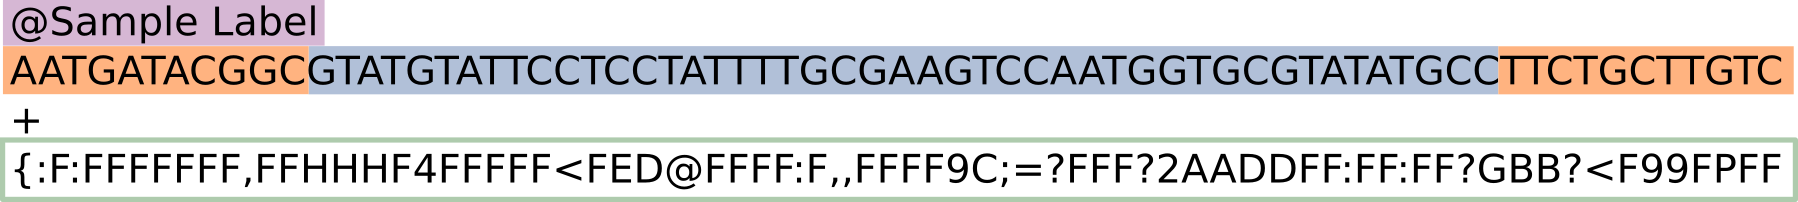
\includegraphics[keepaspectratio]{analysis/../content/images/fastq_example.png}}

}

\caption{Um exemplo de uma sequência de um arquivo FASTQ, com os índices
de qualidade abaixo}

\end{figure}%

As máquinas de sequenciamento (como as da Illumina) leem esses
fragmentos e geram arquivos no formato \textbf{FASTQ}. Cada arquivo
FASTQ contém milhões de sequências curtas chamadas \textbf{reads},
acompanhadas de índices de qualidade (Phred Score) para cada base
identificada. No entanto, esses arquivos brutos contêm:

\begin{itemize}
\tightlist
\item
  Adaptadores de sequenciamento.
\item
  Bases de baixa qualidade nas extremidades.
\item
  \textbf{Contaminação do Hospedeiro:} Em modelos de infecção, até
  95-99\% das reads podem ser do hospedeiro (\emph{Mus musculus}),
  mascarando o sinal da \emph{Candida albicans}.
\end{itemize}

\section{2. O Pipeline
nf-core/detaxizer}\label{o-pipeline-nf-coredetaxizer}

Para resolver o problema da contaminação, utilizamos o pipeline
\href{https://nf-co.re/detaxizer/}{\textbf{nf-core/detaxizer}}. Ele é
projetado especificamente para verificar a presença de táxons
específicos e filtrá-los de arquivos FASTQ.

O fluxo de trabalho do detaxizer segue estas etapas principais:

\begin{enumerate}
\def\labelenumi{\arabic{enumi}.}
\tightlist
\item
  \textbf{Controle de Qualidade (FastQC):} Avaliação inicial da
  qualidade das reads brutas.
\item
  \textbf{Pré-processamento Opcional (fastp):} Corte de adaptadores e
  filtragem de reads por tamanho ou qualidade.
\item
  \textbf{Classificação Taxonômica (Kraken2 e/ou bbduk):} As reads são
  comparadas contra bancos de dados genômicos para identificar sua
  origem. O \textbf{Kraken2} usa k-mers para uma atribuição rápida,
  enquanto o \textbf{bbduk} pode ser usado para pareamento direto contra
  sequências de referência.
\item
  \textbf{Validação Opcional (BLASTN):} Para maior rigor, as reads
  classificadas podem ser validadas via alinhamento BLAST contra bancos
  de dados de nucleotídeos.
\item
  \textbf{Filtragem:} O pipeline remove as reads associadas ao táxon
  indesejado (neste caso, \emph{Mammalia}).
\item
  \textbf{Relatório (MultiQC):} Consolida todos os resultados em um
  único arquivo HTML, permitindo visualizar quantas reads foram
  removidas e a qualidade final dos dados.
\end{enumerate}

\section{3. Automação com Nextflow}\label{automauxe7uxe3o-com-nextflow}

A execução de todas essas ferramentas manualmente seria propensa a erros
e difícil de reproduzir. Para isso, utilizamos o
\href{https://nextflow.io/}{\textbf{Nextflow}}, um motor de fluxo de
trabalho que gerencia a instalação de ferramentas (via
Docker/Singularity) e a execução paralela das tarefas.

\begin{tcolorbox}[enhanced jigsaw, arc=.35mm, bottomrule=.15mm, bottomtitle=1mm, breakable, colback=white, colbacktitle=quarto-callout-note-color!10!white, colframe=quarto-callout-note-color-frame, coltitle=black, left=2mm, leftrule=.75mm, opacityback=0, opacitybacktitle=0.6, rightrule=.15mm, title=\textcolor{quarto-callout-note-color}{\faInfo}\hspace{0.5em}{Ponto Importante}, titlerule=0mm, toprule=.15mm, toptitle=1mm]

Para utilizar o Nextflow, é necessário ter o Java instalado e o comando
\texttt{curl\ -s\ https://get.nextflow.io\ \textbar{}\ bash}. O Nextflow
organiza cada ferramenta em ``processos'' que são conectados em uma
``pipeline''.

\end{tcolorbox}

\subsection{O Script de Execução}\label{o-script-de-execuuxe7uxe3o}

Para o nosso conjunto de dados de \emph{Candida} e macrófagos, o comando
utilizado para a descontaminação foi:

\begin{Shaded}
\begin{Highlighting}[]
\ExtensionTok{nextflow}\NormalTok{ run nf{-}core/detaxizer }\DataTypeTok{\textbackslash{}}
   \AttributeTok{{-}profile}\NormalTok{ docker }\DataTypeTok{\textbackslash{}}
   \AttributeTok{{-}{-}input}\NormalTok{ samplesheet.csv }\DataTypeTok{\textbackslash{}}
   \AttributeTok{{-}{-}preprocessing} \DataTypeTok{\textbackslash{}}
   \AttributeTok{{-}{-}kraken2db}\NormalTok{ db/k2\_pluspf\_20260226.tar.gz }\DataTypeTok{\textbackslash{}}
   \AttributeTok{{-}{-}classification\_kraken2\_post\_filtering} \DataTypeTok{\textbackslash{}}
   \AttributeTok{{-}{-}filter\_trimmed} \DataTypeTok{\textbackslash{}}
   \AttributeTok{{-}{-}save\_intermediates} \DataTypeTok{\textbackslash{}}
   \AttributeTok{{-}{-}classification\_bbduk} \DataTypeTok{\textbackslash{}}
   \AttributeTok{{-}{-}classification\_kraken2} \DataTypeTok{\textbackslash{}}
   \AttributeTok{{-}{-}tax2filter} \StringTok{\textquotesingle{}Mammalia\textquotesingle{}} \DataTypeTok{\textbackslash{}}
   \AttributeTok{{-}{-}outdir}\NormalTok{ results/decontaminated/}
\end{Highlighting}
\end{Shaded}

\subsection{Entendendo os
Parâmetros:}\label{entendendo-os-paruxe2metros}

\begin{itemize}
\tightlist
\item
  \texttt{-profile\ docker}: Garante que todas as ferramentas (Kraken2,
  FastQC, etc.) rodem dentro de containers, sem necessidade de
  instalação manual.
\item
  \texttt{-\/-tax2filter\ \textquotesingle{}Mammalia\textquotesingle{}}:
  O ponto crucial. Instruímos o pipeline a identificar e remover tudo o
  que for classificado como mamífero (o hospedeiro \emph{Mus musculus} e
  qualquer outra leitura humana).
\item
  \texttt{-\/-kraken2db}: Aponta para o banco de dados taxonômico usado
  para a identificação.
\item
  \texttt{-\/-filter\_trimmed}: Aplica a filtragem nas reads já
  processadas pelo \texttt{fastp}.
\end{itemize}

\begin{tcolorbox}[enhanced jigsaw, arc=.35mm, bottomrule=.15mm, bottomtitle=1mm, breakable, colback=white, colbacktitle=quarto-callout-tip-color!10!white, colframe=quarto-callout-tip-color-frame, coltitle=black, left=2mm, leftrule=.75mm, opacityback=0, opacitybacktitle=0.6, rightrule=.15mm, title=\textcolor{quarto-callout-tip-color}{\faLightbulb}\hspace{0.5em}{Tip}, titlerule=0mm, toprule=.15mm, toptitle=1mm]

Sobre o Banco de Dados Kraken2 (PlusPF)

O banco de dados utilizado, k2\_pluspf, é a versão Standard plus Refseq
protozoa \& fungi. Ele contém o genoma humano, genomas de bactérias,
archaea, vírus e, crucialmente para este curso, o RefSeq de protozoários
e fungos.

Isso é fundamental porque, para filtrar o que é Mammalia com segurança,
o software precisa saber diferenciar o que é hospedeiro do que é
patógeno. Sem as sequências de fungos no banco, o Kraken2 poderia
classificar erroneamente reads da Candida como sendo de origem
desconhecida ou até atribuí-las falsamente a outros grupos. Para mais
informações sobre as referências do Kraken2, consulte
\url{https://benlangmead.github.io/aws-indexes/k2}

\end{tcolorbox}

Ao final deste processo, obtemos arquivos FASTQ ``limpos'', contendo
predominantemente sequências da \emph{Candida albicans}, prontos para a
próxima etapa: a \textbf{Quantificação}.

\begin{tcolorbox}[enhanced jigsaw, arc=.35mm, bottomrule=.15mm, bottomtitle=1mm, breakable, colback=white, colbacktitle=quarto-callout-note-color!10!white, colframe=quarto-callout-note-color-frame, coltitle=black, left=2mm, leftrule=.75mm, opacityback=0, opacitybacktitle=0.6, rightrule=.15mm, title=\textcolor{quarto-callout-note-color}{\faInfo}\hspace{0.5em}{Ponto Importante}, titlerule=0mm, toprule=.15mm, toptitle=1mm]

Uma estratégia igualmente válida seria remover as leituras de
\emph{Fungi} e analisar a partir das leituras removidas ao invés das
filtradas. Talvez um de vocês possa tentar isso depois!

\end{tcolorbox}

\section{Visualizando a Composição Taxonômica
(Kraken2)}\label{visualizando-a-composiuxe7uxe3o-taxonuxf4mica-kraken2}

Para avaliar a eficiência da nossa estratégia de descontaminação e
entender a composição das nossas amostras brutas, analisamos a
distribuição taxonômica das reads antes da filtragem. O gráfico abaixo,
gerado pelo MultiQC, resume os principais táxons identificados pelo
Kraken2.

\pandocbounded{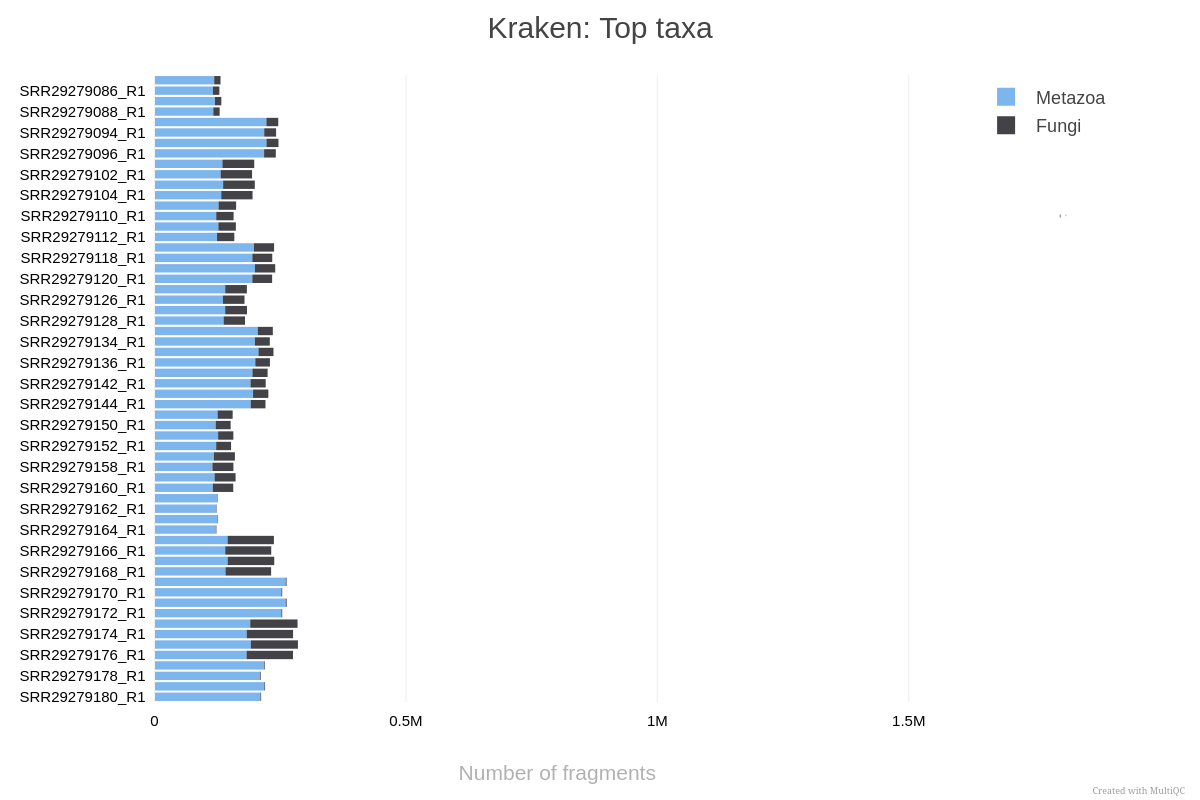
\includegraphics[keepaspectratio]{analysis/../content/images/kraken-top-n-plot.png}}

Como interpretar este gráfico:

\begin{itemize}
\item
  Predomínio de Metazoa (Azul): Como esperado em um modelo de infecção
  de macrófagos, a grande maioria dos fragmentos é classificada como
  Metazoa (neste caso, representando o hospedeiro, Mus musculus). Isso
  ilustra o desafio da ``contaminação do hospedeiro'': o sinal do
  camundongo é ordens de grandeza maior que o do patógeno.
\item
  O Nosso Alvo - Fungi (Cinza Escuro): Os segmentos em cinza escuro
  representam o reino Fungi, especificamente a Candida albicans. Observe
  que a proporção de reads fúngicas varia entre as amostras.
\end{itemize}

\begin{tcolorbox}[enhanced jigsaw, arc=.35mm, bottomrule=.15mm, bottomtitle=1mm, breakable, colback=white, colbacktitle=quarto-callout-tip-color!10!white, colframe=quarto-callout-tip-color-frame, coltitle=black, left=2mm, leftrule=.75mm, opacityback=0, opacitybacktitle=0.6, rightrule=.15mm, title=\textcolor{quarto-callout-tip-color}{\faLightbulb}\hspace{0.5em}{Tip}, titlerule=0mm, toprule=.15mm, toptitle=1mm]

Por que isso é importante?

Ao utilizarmos o pipeline nf-core/detaxizer com o parâmetro --tax2filter
`Mammalia', estamos essencialmente ``removendo'' a parte azul dessas
barras e mantendo apenas a parte cinza escuro. Isso garante que, na
etapa de Quantificação, o software não perca tempo processando
sequências do hospedeiro que não nos interessam para este estudo
específico do patógeno.

\end{tcolorbox}

\begin{center}\rule{0.5\linewidth}{0.5pt}\end{center}

\textbf{Com os dados descontaminados, como podemos saber exatamente
quantos genes da \emph{Candida} estão presentes em cada amostra? Veremos
isso na próxima seção sobre o nf-core/rnaseq.}

\bookmarksetup{startatroot}

\chapter{Quantificação}\label{quantificauxe7uxe3o}

Com os dados descontaminados, o próximo passo é identificar a quais
genes da \emph{Candida albicans} essas sequências pertencem e contar
quantas vezes cada gene aparece em nossas amostras. Este processo é
conhecido como \textbf{Quantificação}.

\section{1. Alinhamento e
Quantificação}\label{alinhamento-e-quantificauxe7uxe3o}

O processo de quantificação geralmente envolve duas etapas principais:

\begin{enumerate}
\def\labelenumi{\arabic{enumi}.}
\tightlist
\item
  \textbf{Alinhamento (Mapping):} As reads (sequências curtas) são
  comparadas contra um genoma de referência ou transcriptoma. É como
  montar um quebra-cabeça onde usamos o genoma como o guia para saber de
  onde cada peça veio.
\item
  \textbf{Contagem (Counting):} Uma vez que sabemos onde a read se
  encaixa, verificamos se ela caiu em uma região anotada como um
  ``gene''. O resultado final é uma \textbf{Matriz de Contagens}, onde
  cada linha é um gene e cada coluna é uma amostra.
\end{enumerate}

\begin{figure}[H]

{\centering \pandocbounded{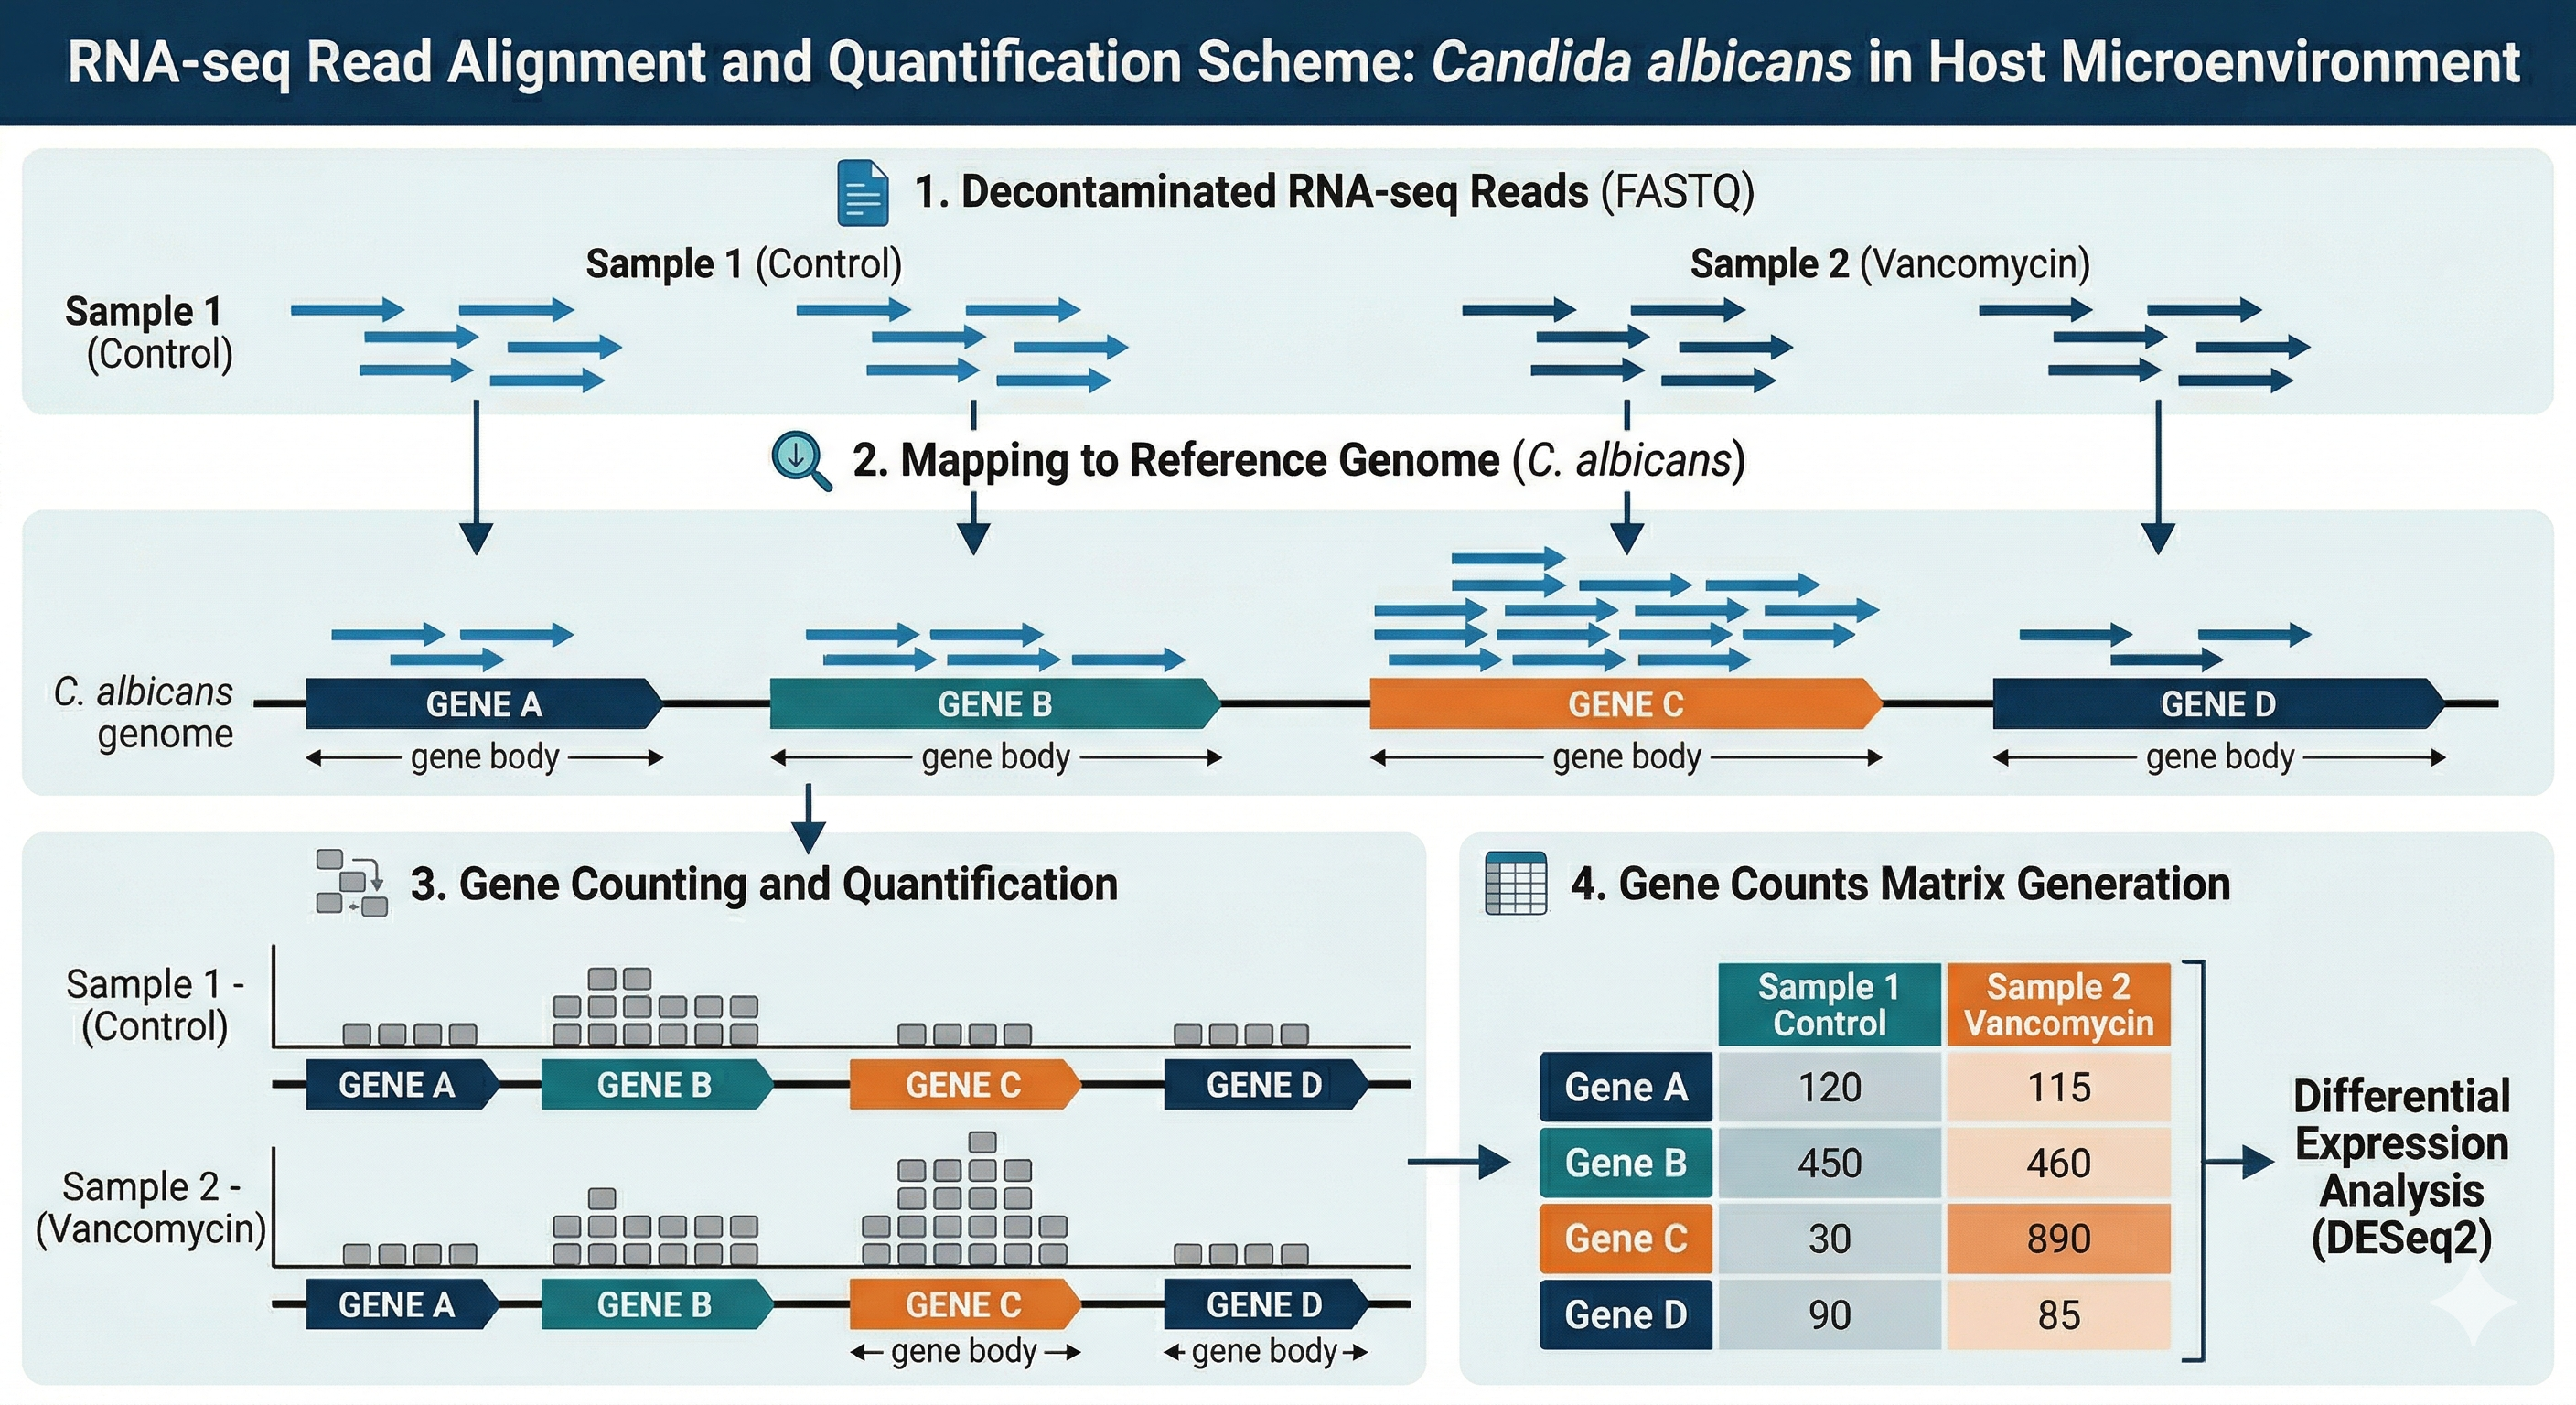
\includegraphics[keepaspectratio]{analysis/../content/images/rnaseq_alignment_scheme.png}}

}

\caption{Esquema simplificado de alinhamento de reads contra um genoma
de referência e a geração da matriz de contagens.}

\end{figure}%

\section{2. O Pipeline nf-core/rnaseq}\label{o-pipeline-nf-corernaseq}

Para esta etapa, utilizamos o
\href{https://nf-co.re/rnaseq}{\textbf{nf-core/rnaseq}}, um dos
pipelines mais robustos e utilizados no mundo para análise de
transcriptômica. Ele automatiza desde o controle de qualidade final até
a geração das matrizes de expressão.

\subsection{O Script de Execução}\label{o-script-de-execuuxe7uxe3o-1}

O comando utilizado para quantificar o transcriptoma da \emph{Candida
albicans} foi:

\begin{Shaded}
\begin{Highlighting}[]
\ExtensionTok{nextflow}\NormalTok{ run nf{-}core/rnaseq }\DataTypeTok{\textbackslash{}}
    \AttributeTok{{-}{-}input}\NormalTok{ rnaseq\_samplesheet.csv }\DataTypeTok{\textbackslash{}}
    \AttributeTok{{-}{-}outdir}\NormalTok{ rnaseq\_results }\DataTypeTok{\textbackslash{}}
    \AttributeTok{{-}{-}gtf}\NormalTok{ db/Candida\_albicans.GCA000182965v3.62.gtf.gz }\DataTypeTok{\textbackslash{}}
    \AttributeTok{{-}{-}fasta}\NormalTok{ db/Candida\_albicans.GCA000182965v3.dna.toplevel.fa.gz }\DataTypeTok{\textbackslash{}}
    \AttributeTok{{-}profile}\NormalTok{ docker }\DataTypeTok{\textbackslash{}}
    \AttributeTok{{-}resume} \AttributeTok{{-}with{-}tower}
\end{Highlighting}
\end{Shaded}

\subsection{Entendendo os
Parâmetros:}\label{entendendo-os-paruxe2metros-1}

\begin{itemize}
\tightlist
\item
  \texttt{-\/-fasta}: O arquivo de sequência genômica (o ``dicionário''
  de DNA) da \emph{Candida}.
\item
  \texttt{-\/-gtf}: O arquivo de anotação, que diz ao software as
  coordenadas exatas de onde cada gene começa e termina no genoma.
\item
  \texttt{-with-tower}: Permite o monitoramento remoto da execução via
  \href{https://tower.nf/}{Nextflow Tower}.
\end{itemize}

\section{3. Fontes de Dados: Ensembl
Fungi}\label{fontes-de-dados-ensembl-fungi}

Para organismos não-modelos ou patógenos fúngicos, a fonte para genomas
e anotações é o \href{https://fungi.ensembl.org/}{\textbf{Ensembl
Fungi}}.

Para este curso, utilizamos a linhagem de referência \textbf{SC5314} da
\emph{Candida albicans}. As referências foram adquiridas nos seguintes
links:

\begin{itemize}
\tightlist
\item
  \textbf{Genoma (Fasta):}
  \href{https://fungi.ensembl.org/Candida_albicans_sc5314_gca_000784655/Info/Index}{C.
  albicans DNA Toplevel}
\item
  \textbf{Anotação (GTF):}
  \href{https://fungi.ensembl.org/Candida_albicans_sc5314_gca_000784655/Info/Index}{C.
  albicans Gene Annotation}
\end{itemize}

\begin{tcolorbox}[enhanced jigsaw, arc=.35mm, bottomrule=.15mm, bottomtitle=1mm, breakable, colback=white, colbacktitle=quarto-callout-important-color!10!white, colframe=quarto-callout-important-color-frame, coltitle=black, left=2mm, leftrule=.75mm, opacityback=0, opacitybacktitle=0.6, rightrule=.15mm, title=\textcolor{quarto-callout-important-color}{\faExclamation}\hspace{0.5em}{Por que usar o Ensembl Fungi?}, titlerule=0mm, toprule=.15mm, toptitle=1mm]

Diferente do Ensembl principal (focado em vertebrados), o Ensembl Fungi
mantém curadoria específica para as complexidades de genomas fúngicos,
como estruturas de íntrons compactas e polimorfismos frequentes,
garantindo que a nossa quantificação seja a mais precisa possível.

\end{tcolorbox}

\subsection{4. Entendendo os Outputs: Do Transcrito ao Gene à
Proteína}\label{entendendo-os-outputs-do-transcrito-ao-gene-uxe0-proteuxedna}

Antes de abrirmos o R para a Análise de Expressão Diferencial,
precisamos alinhar exatamente o que o RNA-Seq mede e como isso se
conecta com o resto do curso.

Lembrando o dogma central da biologia molecular (\textbf{DNA → RNA →
Proteína}), nosso dado é um ``snapshot'' do \textbf{transcriptoma}
(RNA). O Salmon quantifica \textbf{transcritos} (mRNA), mas nas próximas
etapas falaremos constantemente em \textbf{genes} e \textbf{proteínas}.
Por que essa mudança de termos?

\begin{itemize}
\tightlist
\item
  \textbf{Dos Transcritos aos Genes:} Um único gene pode gerar múltiplos
  transcritos (isoformas) por \emph{splicing} alternativo. Para
  simplificar a análise, especialmente no genoma mais compacto da
  \emph{Candida albicans}, o padrão é \textbf{somar as contagens das
  isoformas em um único valor por gene}. O pipeline
  \emph{nf-core/rnaseq} já fez isso para nós e gerou o arquivo que
  usaremos: \texttt{salmon.merged.gene\_counts.tsv}.
\item
  \textbf{Dos Genes às Proteínas:} No final da nossa análise, usaremos
  esses genes para mapear vias biológicas e redes de interação (PPI).
\end{itemize}

\begin{tcolorbox}[enhanced jigsaw, arc=.35mm, bottomrule=.15mm, bottomtitle=1mm, breakable, colback=white, colbacktitle=quarto-callout-note-color!10!white, colframe=quarto-callout-note-color-frame, coltitle=black, left=2mm, leftrule=.75mm, opacityback=0, opacitybacktitle=0.6, rightrule=.15mm, title=\textcolor{quarto-callout-note-color}{\faInfo}\hspace{0.5em}{Atenção aos Termos}, titlerule=0mm, toprule=.15mm, toptitle=1mm]

Na literatura, é muito comum ler ``o gene X está superexpresso'' ou ``a
proteína Y alterou'' em estudos de RNA-Seq. Na prática, nós medimos
apenas a \textbf{abundância de transcritos} e a usamos como um
\emph{proxy} (uma estimativa) da atividade do gene e da futura tradução
proteica. Seguiremos essa mesma convenção prática ao longo do curso.

\end{tcolorbox}

\begin{center}\rule{0.5\linewidth}{0.5pt}\end{center}

\textbf{Com a nossa matriz de contagens pronta e os conceitos alinhados,
vamos abrir o R. A grande pergunta agora é: quais genes alteraram sua
expressão devido ao tratamento com vancomicina? É o que vamos descobrir
a seguir usando o DESeq2.}

\bookmarksetup{startatroot}

\chapter{Análise de Expressão
Diferencial}\label{anuxe1lise-de-expressuxe3o-diferencial}

Nas etapas anteriores, descontaminamos as reads do hospedeiro (\emph{Mus
musculus}) e quantificamos o transcriptoma de \emph{Candida albicans}
com o nf-core/rnaseq. O resultado final desse pipeline é uma
\textbf{matriz de contagens}, onde cada linha representa um gene e cada
coluna uma amostra. A partir dessa matriz, podemos realizar a análise de
expressão diferencial para identificar quais genes da \emph{Candida}
foram regulados (upregulados ou downregulados) em resposta ao tratamento
com vancomicina.

\begin{center}\rule{0.5\linewidth}{0.5pt}\end{center}

\section{Sanidade de Dados}\label{sanidade-de-dados}

Antes de realizarmos a análise de expressão diferencial propriamente
dita, é fundamental explorar a estrutura do nosso conjunto de dados.
Essa etapa, frequentemente chamada de sanidade de dados ou análise
exploratória, serve para responder perguntas essenciais:

\begin{itemize}
\tightlist
\item
  As amostras se agrupam conforme esperamos (por tratamento)?
\item
  Existem \emph{outliers} ou amostras com comportamento atípico?
\item
  Quais variáveis do metadado influenciam a expressão gênica?
\end{itemize}

Para tal, precisamos de técnicas que consigam lidar com a
\textbf{multidimensionalidade} dos dados: estamos analisando milhares de
genes simultaneamente. Técnicas como a Análise de Componentes Principais
(PCA) e a clusterização hierárquica nos permitem ``resumir'' essa
complexidade e visualizar padrões.

\subsection{1. Carregando os Pacotes}\label{carregando-os-pacotes}

Vamos começar carregando os pacotes que utilizaremos ao longo de toda
esta seção prática.

\begin{Shaded}
\begin{Highlighting}[]
\FunctionTok{suppressPackageStartupMessages}\NormalTok{(\{}
  \FunctionTok{library}\NormalTok{(DESeq2)}
  \FunctionTok{library}\NormalTok{(PCAtools)}
  \FunctionTok{library}\NormalTok{(dplyr)}
  \FunctionTok{library}\NormalTok{(readr)}
  \FunctionTok{library}\NormalTok{(tibble)}
  \FunctionTok{library}\NormalTok{(ggplot2)}
  \FunctionTok{library}\NormalTok{(pheatmap)}
\NormalTok{\})}
\end{Highlighting}
\end{Shaded}

\subsection{2. Importando a Matriz de
Contagens}\label{importando-a-matriz-de-contagens}

O nf-core/rnaseq com o quantificador Salmon gera uma tabela consolidada
com as contagens de todos os genes por amostra. Vamos carregá-la:

\begin{Shaded}
\begin{Highlighting}[]
\CommentTok{\# Importar matriz de contagens (gerada pelo Salmon via nf{-}core/rnaseq)}
\NormalTok{gene\_counts }\OtherTok{\textless{}{-}} \FunctionTok{read\_tsv}\NormalTok{(here}\SpecialCharTok{::}\FunctionTok{here}\NormalTok{(}\StringTok{"data/rnaseq/salmon.merged.gene\_counts.tsv"}\NormalTok{),}
                        \AttributeTok{show\_col\_types =} \ConstantTok{FALSE}\NormalTok{)}

\CommentTok{\# Visualizar as primeiras linhas e colunas}
\NormalTok{gene\_counts[}\DecValTok{1}\SpecialCharTok{:}\DecValTok{5}\NormalTok{, }\DecValTok{1}\SpecialCharTok{:}\DecValTok{6}\NormalTok{]}
\end{Highlighting}
\end{Shaded}

\begin{verbatim}
# A tibble: 5 x 6
  gene_id     gene_name   SRR29279085 SRR29279086 SRR29279087 SRR29279088
  <chr>       <chr>             <dbl>       <dbl>       <dbl>       <dbl>
1 C1_00010W_A C1_00010W_A           0           0           0           0
2 C1_00020C_A C1_00020C_A           2           4           1           2
3 C1_00030C_A C1_00030C_A           0           0           0           0
4 C1_00040W_A CTA2                  0           0           0           0
5 C1_00050C_A C1_00050C_A           0           0           0           0
\end{verbatim}

A primeira coluna (\texttt{gene\_id}) contém os identificadores dos
genes de \emph{Candida albicans} no Ensembl Fungi, e a segunda
(\texttt{gene\_name}) contém o nome do gene quando disponível. As demais
colunas são as amostras, identificadas pelo código SRR.

\subsection{3. Importando os Metadados}\label{importando-os-metadados}

As informações sobre as condições experimentais de cada amostra estão no
arquivo \texttt{SraRunTable.csv}, obtido do SRA. Precisamos filtrá-lo
para manter apenas as amostras que foram estimuladas com \emph{Candida
albicans}. Vamos organizar o metadado para que ele possa ser facilmente
integrado com a matriz de contagens. O DESeq2 exige que as colunas da
matriz de contagens correspondam às linhas do metadado, e que o metadado
contenha as variáveis que queremos testar (neste caso, o tratamento) e
as covariáveis (como o grupo experimental).

Além da variável de interesse (\texttt{treatment}), nosso metadado
contém uma informação crucial: o \textbf{lote experimental}
(\texttt{experiment\_group}). Como vimos na descrição do conjunto de
dados, o experimento foi conduzido em \textbf{6 lotes independentes},
cada um contendo 4 amostras tratadas com vancomicina e 4 controles.
Diferenças entre lotes, como variações no dia de cultivo, preparo de
reagentes ou condições de extração, podem introduzir variabilidade que
\textbf{não é interessante para o objetivo do estudo}. Se não levarmos
isso em conta, corremos o risco de confundir efeito de \emph{batch} com
efeito do tratamento, o que pode gerar tanto falsos positivos quanto
falsos negativos nos resultados da expressão diferencial.

\begin{Shaded}
\begin{Highlighting}[]
\CommentTok{\# Importar metadados e filtrar amostras estimuladas com C. albicans}
\NormalTok{sra\_table }\OtherTok{\textless{}{-}} \FunctionTok{read\_csv}\NormalTok{(here}\SpecialCharTok{::}\FunctionTok{here}\NormalTok{(}\StringTok{"data/SraRunTable.csv"}\NormalTok{), }\AttributeTok{show\_col\_types =} \ConstantTok{FALSE}\NormalTok{)}

\NormalTok{metadata }\OtherTok{\textless{}{-}}\NormalTok{ sra\_table }\SpecialCharTok{\%\textgreater{}\%}
  \FunctionTok{filter}\NormalTok{(stimulus }\SpecialCharTok{==} \StringTok{"Candida albicans"}\NormalTok{) }\SpecialCharTok{\%\textgreater{}\%}
\NormalTok{  dplyr}\SpecialCharTok{::}\FunctionTok{select}\NormalTok{(Run, treatment, experiment\_group) }\SpecialCharTok{\%\textgreater{}\%}
  \FunctionTok{mutate}\NormalTok{(}\AttributeTok{treatment =} \FunctionTok{factor}\NormalTok{(treatment, }
                            \AttributeTok{levels =} \FunctionTok{c}\NormalTok{(}\StringTok{"Untreated (control)"}\NormalTok{, }\StringTok{"Vancomycin"}\NormalTok{)),}
         \AttributeTok{experiment\_group =} \FunctionTok{factor}\NormalTok{(experiment\_group,}
                            \AttributeTok{levels =} \FunctionTok{c}\NormalTok{(}\DecValTok{1}\NormalTok{, }\DecValTok{2}\NormalTok{, }\DecValTok{3}\NormalTok{, }\DecValTok{4}\NormalTok{, }\DecValTok{5}\NormalTok{, }\DecValTok{6}\NormalTok{))}
\NormalTok{                            ) }\SpecialCharTok{\%\textgreater{}\%}
  
  \FunctionTok{column\_to\_rownames}\NormalTok{(}\StringTok{"Run"}\NormalTok{)}

\NormalTok{metadata[}\FunctionTok{order}\NormalTok{(metadata}\SpecialCharTok{$}\NormalTok{experiment\_group),]}
\end{Highlighting}
\end{Shaded}

\begin{verbatim}
                      treatment experiment_group
SRR29279165          Vancomycin                1
SRR29279173 Untreated (control)                1
SRR29279166          Vancomycin                1
SRR29279167          Vancomycin                1
SRR29279168          Vancomycin                1
SRR29279174 Untreated (control)                1
SRR29279175 Untreated (control)                1
SRR29279176 Untreated (control)                1
SRR29279149          Vancomycin                2
SRR29279157 Untreated (control)                2
SRR29279150          Vancomycin                2
SRR29279151          Vancomycin                2
SRR29279152          Vancomycin                2
SRR29279158 Untreated (control)                2
SRR29279159 Untreated (control)                2
SRR29279160 Untreated (control)                2
SRR29279133          Vancomycin                3
SRR29279141 Untreated (control)                3
SRR29279134          Vancomycin                3
SRR29279135          Vancomycin                3
SRR29279136          Vancomycin                3
SRR29279142 Untreated (control)                3
SRR29279143 Untreated (control)                3
SRR29279144 Untreated (control)                3
SRR29279117          Vancomycin                4
SRR29279125 Untreated (control)                4
SRR29279118          Vancomycin                4
SRR29279119          Vancomycin                4
SRR29279120          Vancomycin                4
SRR29279126 Untreated (control)                4
SRR29279127 Untreated (control)                4
SRR29279128 Untreated (control)                4
SRR29279101          Vancomycin                5
SRR29279109 Untreated (control)                5
SRR29279102          Vancomycin                5
SRR29279103          Vancomycin                5
SRR29279104          Vancomycin                5
SRR29279110 Untreated (control)                5
SRR29279111 Untreated (control)                5
SRR29279112 Untreated (control)                5
SRR29279085          Vancomycin                6
SRR29279093 Untreated (control)                6
SRR29279086          Vancomycin                6
SRR29279087          Vancomycin                6
SRR29279088          Vancomycin                6
SRR29279094 Untreated (control)                6
SRR29279095 Untreated (control)                6
SRR29279096 Untreated (control)                6
\end{verbatim}

\begin{tcolorbox}[enhanced jigsaw, arc=.35mm, bottomrule=.15mm, bottomtitle=1mm, breakable, colback=white, colbacktitle=quarto-callout-note-color!10!white, colframe=quarto-callout-note-color-frame, coltitle=black, left=2mm, leftrule=.75mm, opacityback=0, opacitybacktitle=0.6, rightrule=.15mm, title=\textcolor{quarto-callout-note-color}{\faInfo}\hspace{0.5em}{Ponto Importante}, titlerule=0mm, toprule=.15mm, toptitle=1mm]

Repare que cada amostra biológica (\texttt{experiment\_group}) possui 4
runs de sequenciamento (SRR). No nosso caso, o nf-core/rnaseq
quantificou cada run individualmente. Isso significa que temos
\textbf{réplicas técnicas} que devem ser levadas em consideração.
Poderíamos agregá-las somando as contagens, mas como o DESeq2 lida
naturalmente com o modelo de expressão, vamos mantê-las separadas e
incluir o \texttt{experiment\_group} no design para absorver essa
variabilidade.

\end{tcolorbox}

\subsection{4. Preparando a Matriz de
Contagens}\label{preparando-a-matriz-de-contagens}

Agora precisamos transformar a tabela importada em uma matriz numérica
compatível com o DESeq2, e garantir que apenas as amostras de interesse
(com estímulo por \emph{Candida}) estejam presentes.

\begin{Shaded}
\begin{Highlighting}[]
\CommentTok{\# Transformar em matriz numérica com gene\_id como rownames}
\NormalTok{count\_matrix }\OtherTok{\textless{}{-}}\NormalTok{ gene\_counts }\SpecialCharTok{\%\textgreater{}\%}
\NormalTok{  dplyr}\SpecialCharTok{::}\FunctionTok{select}\NormalTok{(gene\_id, }\FunctionTok{all\_of}\NormalTok{(}\FunctionTok{rownames}\NormalTok{(metadata))) }\SpecialCharTok{\%\textgreater{}\%}
  \FunctionTok{column\_to\_rownames}\NormalTok{(}\StringTok{"gene\_id"}\NormalTok{) }\SpecialCharTok{\%\textgreater{}\%}
  \FunctionTok{as.matrix}\NormalTok{()}

\CommentTok{\# O DESeq2 requer valores inteiros}
\NormalTok{count\_matrix }\OtherTok{\textless{}{-}} \FunctionTok{round}\NormalTok{(count\_matrix)}

\CommentTok{\# Verificar correspondência entre metadado e contagens}
\FunctionTok{identical}\NormalTok{(}\FunctionTok{colnames}\NormalTok{(count\_matrix), }\FunctionTok{rownames}\NormalTok{(metadata))}
\end{Highlighting}
\end{Shaded}

\begin{verbatim}
[1] TRUE
\end{verbatim}

\begin{Shaded}
\begin{Highlighting}[]
\FunctionTok{dim}\NormalTok{(count\_matrix)}
\end{Highlighting}
\end{Shaded}

\begin{verbatim}
[1] 6468   48
\end{verbatim}

Temos \textbf{6468 genes} e \textbf{48 amostras} prontos para análise.

\subsection{5. Criando o Objeto DESeq2}\label{criando-o-objeto-deseq2}

O DESeq2 trabalha com um objeto especial (\texttt{DESeqDataSet}) que
armazena juntos a matriz de contagens, o metadado e o modelo
estatístico. Aqui, nosso modelo inclui o \texttt{experiment\_group} como
covariável e o \texttt{treatment} como a variável de interesse:

\begin{Shaded}
\begin{Highlighting}[]
\NormalTok{dds }\OtherTok{\textless{}{-}} \FunctionTok{DESeqDataSetFromMatrix}\NormalTok{(}\AttributeTok{countData =}\NormalTok{ count\_matrix,}
                              \AttributeTok{colData =}\NormalTok{ metadata,}
                              \AttributeTok{design =} \SpecialCharTok{\textasciitilde{}}\NormalTok{ experiment\_group }\SpecialCharTok{+}\NormalTok{ treatment)}
\end{Highlighting}
\end{Shaded}

Antes de prosseguirmos, vamos aplicar a \textbf{Variance Stabilizing
Transformation (VST)}. Dados de RNA-seq possuem uma característica
chamada \textbf{heteroscedasticidade}: a variância das contagens aumenta
conforme a média de expressão cresce (ou seja, genes altamente expressos
apresentam maior variância absoluta). Por outro lado, se aplicássemos
apenas uma transformação logarítmica simples, os genes de baixa
expressão ficariam com uma variância artificialmente inflada. A
transformação VST corrige esse comportamento, tornando a variância mais
homogênea em todos os níveis de expressão. Isso é essencial para
análises exploratórias, como a PCA e a clusterização, mas \emph{não}
para o teste de expressão diferencial em si (que exige as contagens
brutas não normalizadas).

\begin{Shaded}
\begin{Highlighting}[]
\NormalTok{dds\_vst }\OtherTok{\textless{}{-}} \FunctionTok{varianceStabilizingTransformation}\NormalTok{(dds)}
\NormalTok{counts\_vst }\OtherTok{\textless{}{-}} \FunctionTok{assay}\NormalTok{(dds\_vst)}
\end{Highlighting}
\end{Shaded}

\subsection{6. Análise de Componentes Principais
(PCA)}\label{anuxe1lise-de-componentes-principais-pca}

A PCA é uma técnica de \textbf{redução de dimensionalidade} que projeta
os milhares de genes em um número menor de componentes. Cada componente
principal captura um eixo de variabilidade nos dados:

\begin{itemize}
\tightlist
\item
  \textbf{PC1} captura a \emph{maior} fonte de variação.
\item
  \textbf{PC2} captura a segunda maior, e assim por diante.
\end{itemize}

Se o tratamento com vancomicina realmente altera o perfil transcricional
da \emph{Candida}, esperamos ver as amostras se separarem por grupo ao
longo de uma das primeiras componentes.

\begin{Shaded}
\begin{Highlighting}[]
\NormalTok{pca\_result }\OtherTok{\textless{}{-}} \FunctionTok{pca}\NormalTok{(counts\_vst, }\AttributeTok{metadata =}\NormalTok{ metadata)}

\FunctionTok{biplot}\NormalTok{(pca\_result,}
       \AttributeTok{colby =} \StringTok{"treatment"}\NormalTok{,}
       \AttributeTok{shape =} \StringTok{"experiment\_group"}\NormalTok{,}
       \AttributeTok{legendPosition =} \StringTok{"right"}\NormalTok{,}
       \AttributeTok{title =} \StringTok{"PCA — Transcriptoma de C. albicans"}\NormalTok{)}
\end{Highlighting}
\end{Shaded}

\pandocbounded{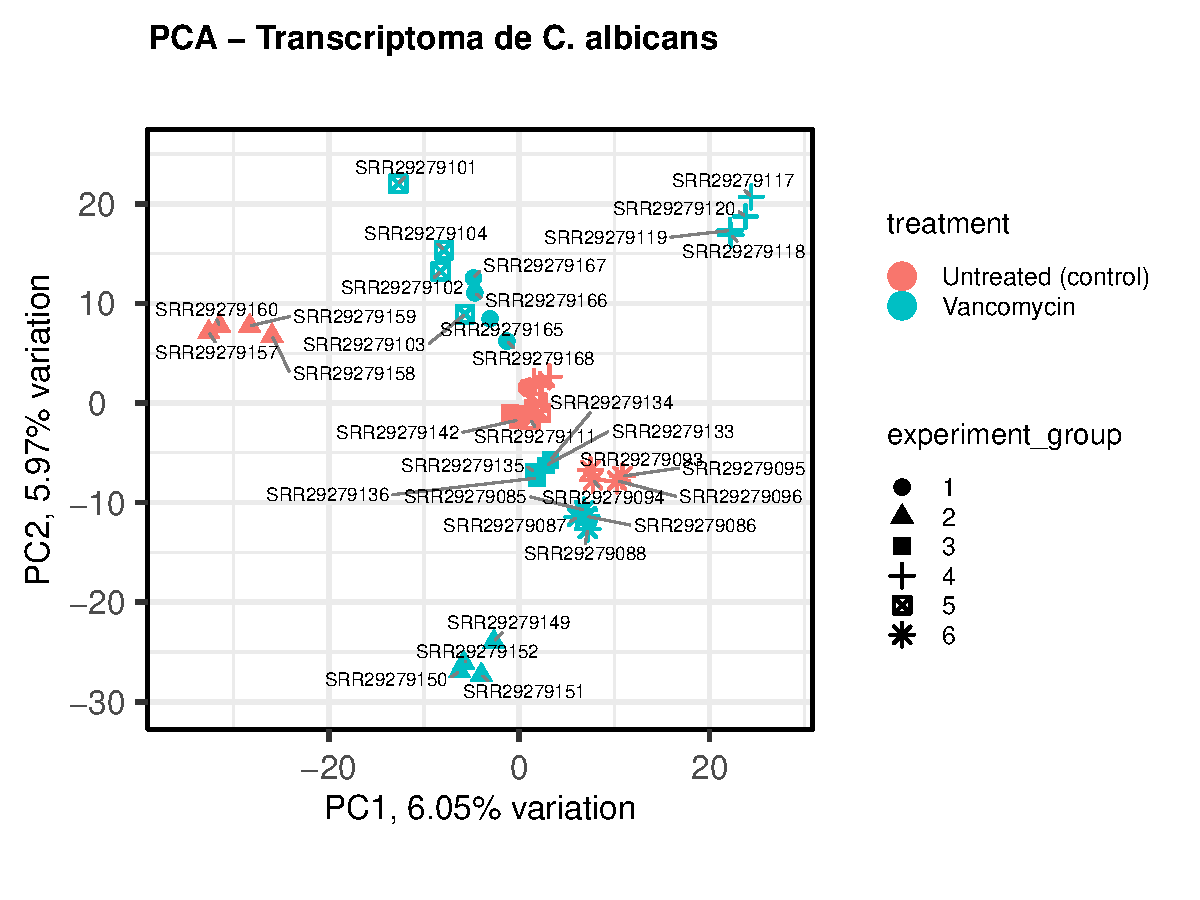
\includegraphics[keepaspectratio]{analysis/03_differential_expression_files/figure-pdf/unnamed-chunk-8-1.pdf}}

\subsubsection{Como interpretar o
biplot:}\label{como-interpretar-o-biplot}

\begin{itemize}
\tightlist
\item
  \textbf{Proximidade entre pontos} indica similaridade no perfil de
  expressão global. Amostras do mesmo grupo de tratamento devem se
  agrupar.
\item
  \textbf{Eixos PC1 e PC2}: o percentual ao lado de cada eixo indica
  quanto da variância total aquela componente explica. Se PC1 sozinha
  explica, por exemplo, 40\% da variância, ela é a dimensão dominante do
  seu dado.
\item
  A \textbf{forma} dos pontos diferencia os grupos experimentais
  (réplicas biológicas), o que permite avaliar se a variação entre
  réplicas é menor do que a variação entre tratamentos --- o cenário
  ideal.
\end{itemize}

\subsection{7. Scree Plot}\label{scree-plot}

O \textbf{scree plot} mostra a proporção de variância explicada por cada
componente principal. Ele ajuda a responder: \emph{quantas dimensões são
necessárias para descrever a variabilidade do meu dado?}

\begin{Shaded}
\begin{Highlighting}[]
\FunctionTok{screeplot}\NormalTok{(pca\_result,}
          \AttributeTok{components =} \FunctionTok{getComponents}\NormalTok{(pca\_result),}
          \AttributeTok{title =} \StringTok{"Scree Plot — Variância por Componente"}\NormalTok{)}
\end{Highlighting}
\end{Shaded}

\pandocbounded{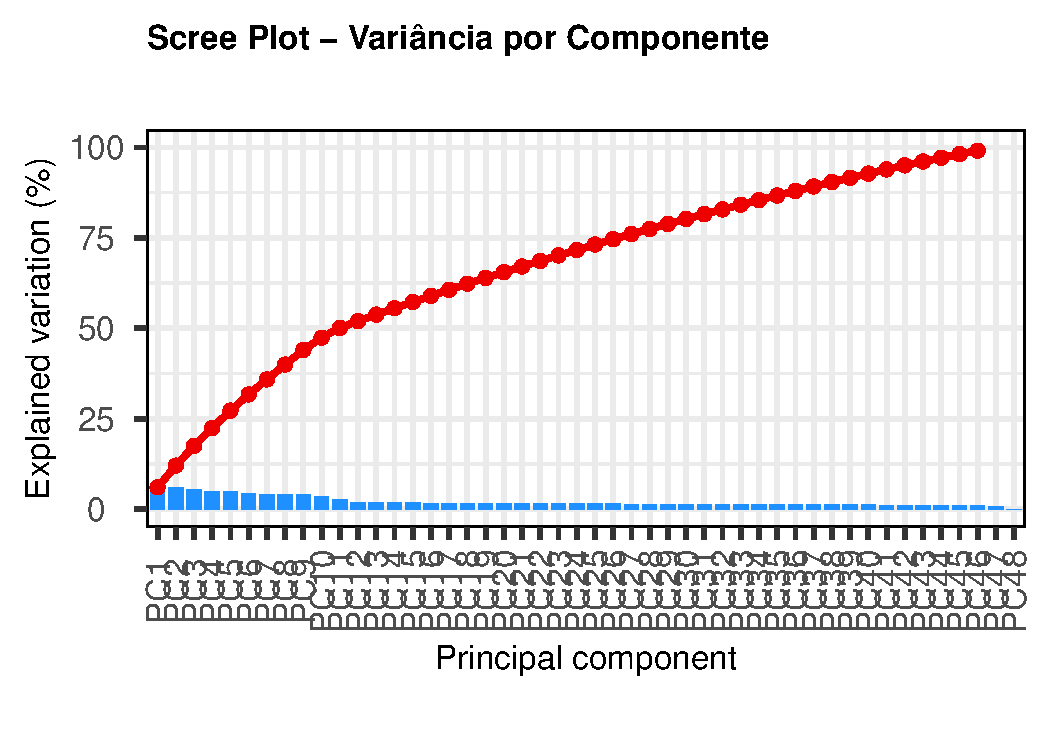
\includegraphics[keepaspectratio]{analysis/03_differential_expression_files/figure-pdf/unnamed-chunk-9-1.pdf}}

\begin{tcolorbox}[enhanced jigsaw, arc=.35mm, bottomrule=.15mm, bottomtitle=1mm, breakable, colback=white, colbacktitle=quarto-callout-tip-color!10!white, colframe=quarto-callout-tip-color-frame, coltitle=black, left=2mm, leftrule=.75mm, opacityback=0, opacitybacktitle=0.6, rightrule=.15mm, title=\textcolor{quarto-callout-tip-color}{\faLightbulb}\hspace{0.5em}{Como interpretar o scree plot}, titlerule=0mm, toprule=.15mm, toptitle=1mm]

Procure pelo ponto onde a curva se achata (\emph{elbow}). Geralmente, em
dados de RNA-seq, as 2--4 primeiras componentes são suficientes para
descrever a maior parte da variabilidade. No nosso caso, é normal que as
duas primeiras componentes não expliquem uma fração muito alta da
variância. Isso acontece porque temos \textbf{6 lotes experimentais
independentes}, cada um introduzindo sua própria fonte de variabilidade.
A variância total acaba sendo ``fragmentada'' entre muitas componentes,
cada uma capturando a variação de um ou mais lotes. Se analisássemos um
único lote, veríamos PC1 e PC2 explicando uma proporção bem maior.

\end{tcolorbox}

\subsubsection{PCA dentro de um único
lote}\label{pca-dentro-de-um-uxfanico-lote}

Para ilustrar esse ponto, vamos repetir a PCA usando apenas as amostras
do \textbf{lote 1} (um par vancomicina/controle com suas réplicas
técnicas):

\begin{Shaded}
\begin{Highlighting}[]
\CommentTok{\# Filtrar apenas amostras do lote 2}
\NormalTok{meta\_batch1 }\OtherTok{\textless{}{-}}\NormalTok{ metadata[metadata}\SpecialCharTok{$}\NormalTok{experiment\_group }\SpecialCharTok{==} \StringTok{"1"}\NormalTok{, , drop }\OtherTok{=} \ConstantTok{FALSE}\NormalTok{]}
\NormalTok{counts\_batch1 }\OtherTok{\textless{}{-}}\NormalTok{ counts\_vst[, }\FunctionTok{rownames}\NormalTok{(meta\_batch1)]}

\NormalTok{pca\_batch1 }\OtherTok{\textless{}{-}} \FunctionTok{pca}\NormalTok{(counts\_batch1, }\AttributeTok{metadata =}\NormalTok{ meta\_batch1)}

\FunctionTok{biplot}\NormalTok{(pca\_batch1,}
       \AttributeTok{colby =} \StringTok{"treatment"}\NormalTok{,}
       \AttributeTok{legendPosition =} \StringTok{"right"}\NormalTok{,}
       \AttributeTok{title =} \StringTok{"PCA — Apenas Lote 1"}\NormalTok{)}
\end{Highlighting}
\end{Shaded}

\pandocbounded{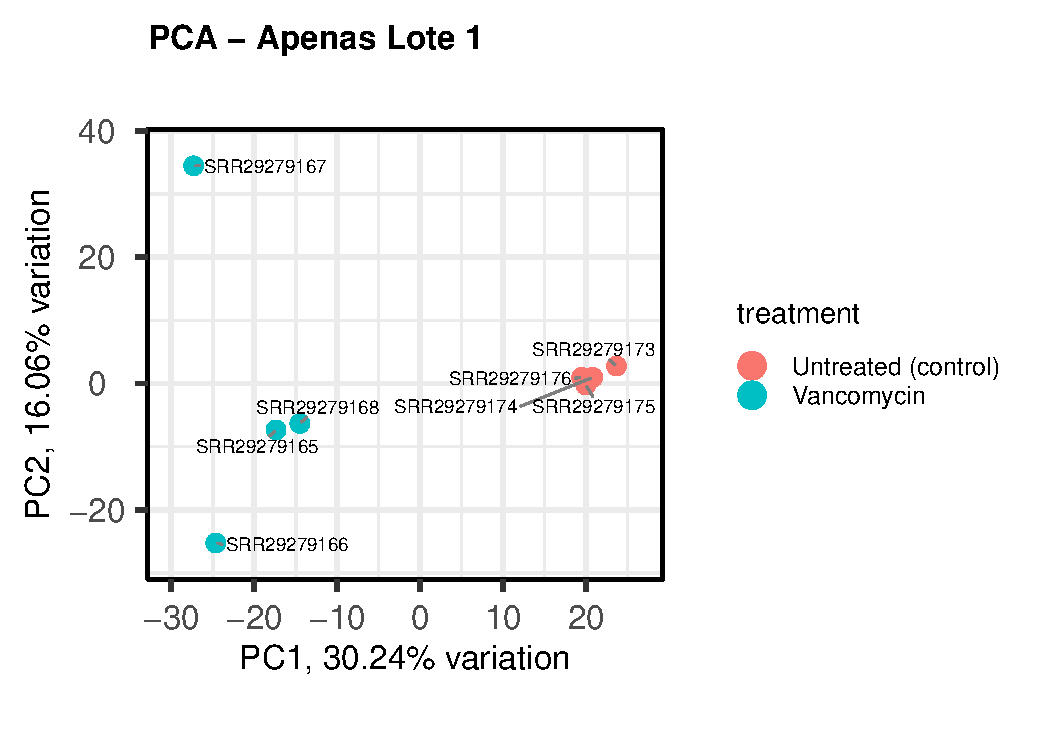
\includegraphics[keepaspectratio]{analysis/03_differential_expression_files/figure-pdf/unnamed-chunk-10-1.pdf}}

Note como, isolando um único lote, a separação entre vancomicina e
controle se torna mais evidente e as primeiras componentes explicam uma
proporção maior da variância. Isso reforça a necessidade de incluir o
\texttt{experiment\_group} como covariável no nosso modelo.

\subsection{8. Clusterização
Hierárquica}\label{clusterizauxe7uxe3o-hieruxe1rquica}

A clusterização hierárquica agrupa as amostras com base na
\textbf{distância euclidiana} entre seus perfis de expressão,
construindo um \textbf{dendrograma}. Amostras com perfis mais similares
são conectadas mais próximas na árvore.

\begin{Shaded}
\begin{Highlighting}[]
 \CommentTok{\# Transpor a matriz: cada amostra vira uma linha}

\NormalTok{counts\_vst\_t }\OtherTok{\textless{}{-}} \FunctionTok{t}\NormalTok{(counts\_vst)}


\CommentTok{\# Calcular distâncias euclidianas}

\NormalTok{d }\OtherTok{\textless{}{-}} \FunctionTok{dist}\NormalTok{(counts\_vst\_t, }\AttributeTok{method =} \StringTok{"euclidean"}\NormalTok{)}


\CommentTok{\# Clusterizar com ligação completa}

\NormalTok{clusters }\OtherTok{\textless{}{-}} \FunctionTok{hclust}\NormalTok{(d, }\AttributeTok{method =} \StringTok{"complete"}\NormalTok{)}



\CommentTok{\# 1. Criar um vetor de novos rótulos combinando as colunas}
\CommentTok{\# Garantimos que a ordem dos metadados seja a mesma das amostras na matriz}
\NormalTok{novos\_rotulos }\OtherTok{\textless{}{-}} \FunctionTok{paste}\NormalTok{(metadata[}\FunctionTok{rownames}\NormalTok{(counts\_vst\_t), }\StringTok{"treatment"}\NormalTok{], }
\NormalTok{                       metadata[}\FunctionTok{rownames}\NormalTok{(counts\_vst\_t), }\StringTok{"experiment\_group"}\NormalTok{], }
                       \AttributeTok{sep =} \StringTok{" | "}\NormalTok{)}

\CommentTok{\# 2. Plotar o dendrograma usando o argumento \textquotesingle{}labels\textquotesingle{}}
\FunctionTok{par}\NormalTok{(}\AttributeTok{mar =} \FunctionTok{c}\NormalTok{(}\DecValTok{4}\NormalTok{, }\DecValTok{4}\NormalTok{, }\DecValTok{2}\NormalTok{, }\DecValTok{8}\NormalTok{)) }\CommentTok{\# Aumentar a margem direita se os nomes forem longos}
\FunctionTok{plot}\NormalTok{(clusters,}
     \AttributeTok{labels =}\NormalTok{ novos\_rotulos,}
     \AttributeTok{main =} \StringTok{"Clusterização Hierárquica — Tratamento e Batch"}\NormalTok{,}
     \AttributeTok{xlab =} \StringTok{""}\NormalTok{,}
     \AttributeTok{sub =} \StringTok{""}\NormalTok{,}
     \AttributeTok{cex =} \DecValTok{1}\NormalTok{) }\CommentTok{\# Font size}
\end{Highlighting}
\end{Shaded}

\pandocbounded{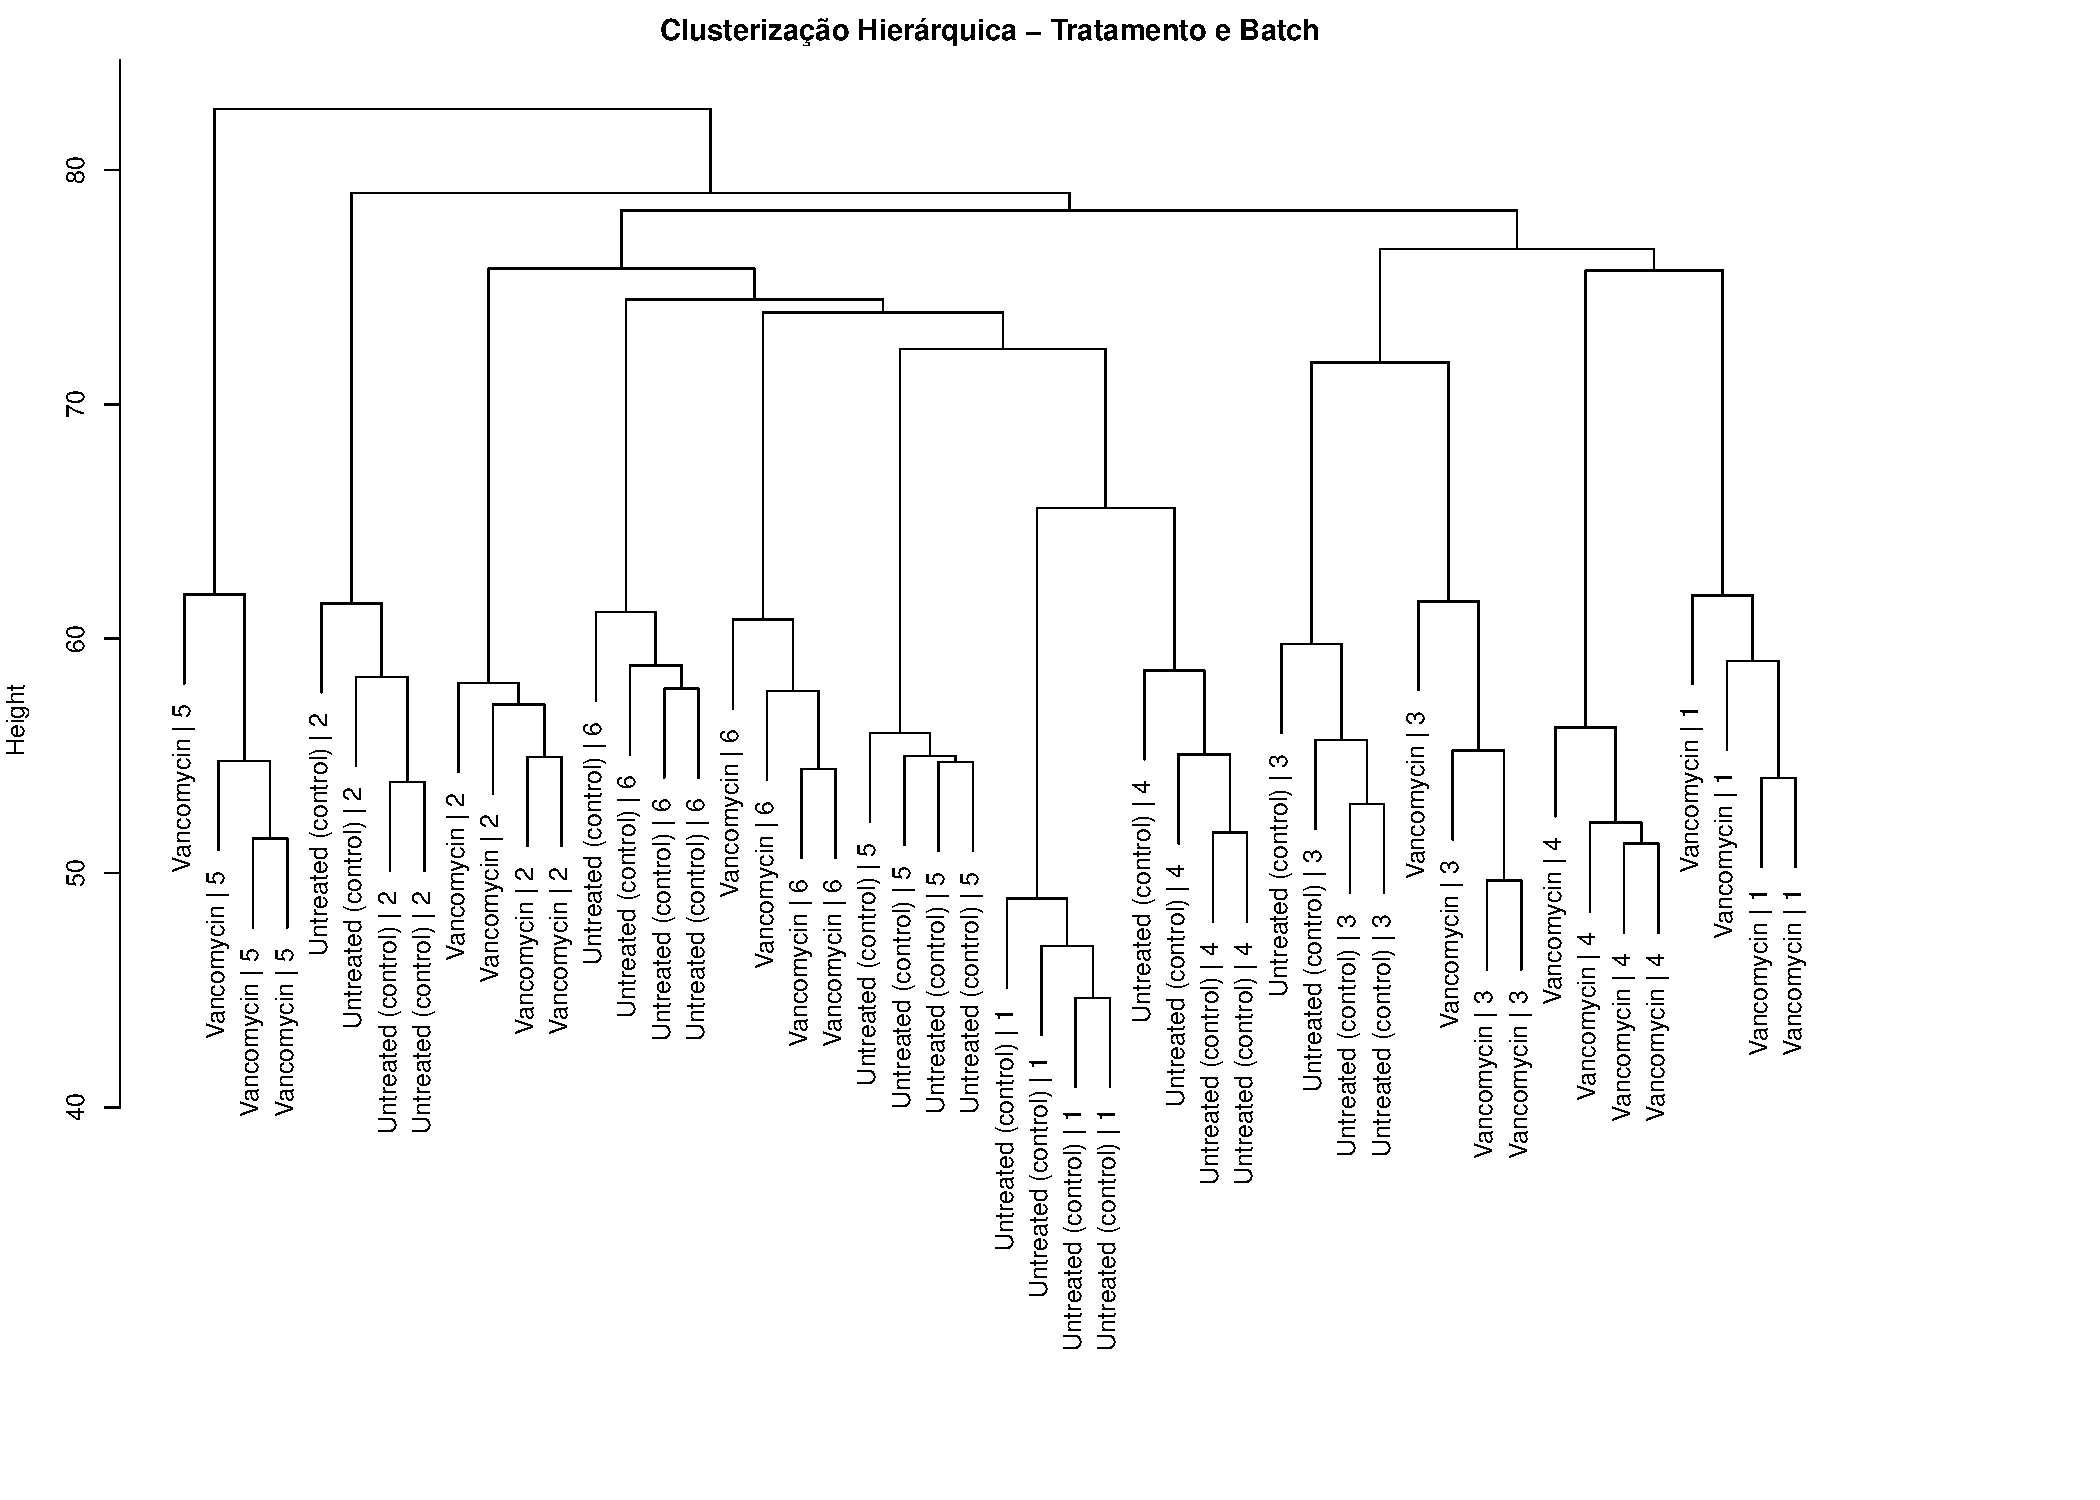
\includegraphics[keepaspectratio]{analysis/03_differential_expression_files/figure-pdf/unnamed-chunk-11-1.pdf}}

\subsubsection{Como interpretar o
dendrograma:}\label{como-interpretar-o-dendrograma}

\begin{itemize}
\tightlist
\item
  Amostras que compartilham um ramo próximo possuem perfil de expressão
  semelhante.
\item
  O ideal é que as amostras se agrupem por \textbf{tratamento}
  (vancomicina vs.~controle) e não por outras variáveis como o lote
  experimental.
\item
  Se amostras de grupos diferentes estiverem misturadas, isso pode
  indicar um efeito biológico fraco ou um forte efeito de \emph{batch}.
\end{itemize}

\subsection{9. Análise de
Covariáveis}\label{anuxe1lise-de-covariuxe1veis}

Uma análise de expressão diferencial é, em essência, \textbf{um modelo
de regressão} aplicado a cada gene. A variável principal é o tratamento
(vancomicina vs.~controle), mas outras variáveis, como o grupo
experimental (lote/batch), podem influenciar significativamente a
expressão.

A função \texttt{eigencorplot} nos permite visualizar quais variáveis do
metadado se correlacionam com as primeiras componentes principais,
ajudando na decisão de \textbf{quais covariáveis incluir no modelo}.

\begin{Shaded}
\begin{Highlighting}[]
\FunctionTok{eigencorplot}\NormalTok{(pca\_result,}
             \AttributeTok{metavars =} \FunctionTok{c}\NormalTok{(}\StringTok{"treatment"}\NormalTok{, }\StringTok{"experiment\_group"}\NormalTok{),}
             \AttributeTok{main =} \StringTok{"Correlação entre Covariáveis e Componentes Principais"}\NormalTok{)}
\end{Highlighting}
\end{Shaded}

\pandocbounded{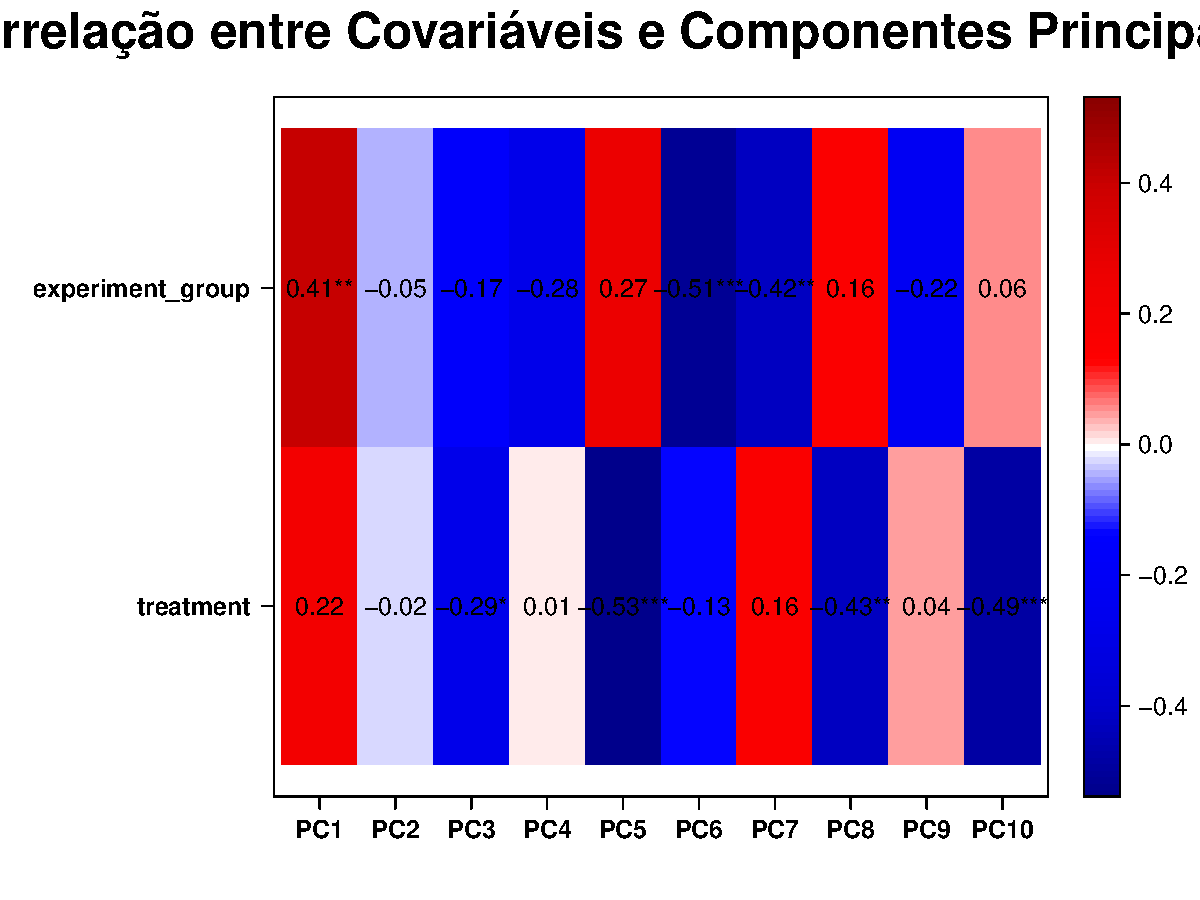
\includegraphics[keepaspectratio]{analysis/03_differential_expression_files/figure-pdf/unnamed-chunk-12-1.pdf}}

\begin{tcolorbox}[enhanced jigsaw, arc=.35mm, bottomrule=.15mm, bottomtitle=1mm, breakable, colback=white, colbacktitle=quarto-callout-important-color!10!white, colframe=quarto-callout-important-color-frame, coltitle=black, left=2mm, leftrule=.75mm, opacityback=0, opacitybacktitle=0.6, rightrule=.15mm, title=\textcolor{quarto-callout-important-color}{\faExclamation}\hspace{0.5em}{Por que incluir covariáveis?}, titlerule=0mm, toprule=.15mm, toptitle=1mm]

Se o \texttt{experiment\_group} (lote biológico) se correlaciona
fortemente com alguma das primeiras componentes, isso significa que
parte da variabilidade que observamos vem do lote de cultivo celular, e
não do efeito da vancomicina. Ao incluir essa variável no modelo do
DESeq2 (\texttt{\textasciitilde{}\ experiment\_group\ +\ treatment}),
``descontamos'' esse efeito e aumentamos o poder estatístico para
detectar os genes realmente alterados pelo tratamento.

\end{tcolorbox}

\begin{center}\rule{0.5\linewidth}{0.5pt}\end{center}

\textbf{A sanidade dos nossos dados nos deu uma visão geral da sua
estrutura. As amostras se comportam como esperado? Há outliers que
precisam de atenção? Com essas respostas em mãos, podemos avançar com
confiança para a próxima etapa.}

\begin{center}\rule{0.5\linewidth}{0.5pt}\end{center}

\section{Análise de Expressão Diferencial de Genes
(DGE)}\label{anuxe1lise-de-expressuxe3o-diferencial-de-genes-dge}

Agora chegamos à pergunta central deste curso: \textbf{quais genes da
\emph{Candida albicans} mudaram de comportamento em resposta à
vancomicina?}

A análise de Expressão Diferencial de Genes (DGE) é, essencialmente, um
modelo de regressão aplicado a cada gene individualmente. O DESeq2
implementa um \textbf{Modelo Linear Generalizado (GLM)} baseado na
distribuição \textbf{Binomial Negativa}, que é particularmente adequada
para dados de contagem de RNA-seq, onde a variância geralmente excede a
média (sobredispersão).

\subsection{10. Rodando o DESeq2}\label{rodando-o-deseq2}

A função \texttt{DESeq()} congrega três etapas internas:

\begin{enumerate}
\def\labelenumi{\arabic{enumi}.}
\tightlist
\item
  \textbf{Estimativa dos fatores de normalização}
  (\texttt{estimateSizeFactors}): corrige diferenças na profundidade de
  sequenciamento entre amostras.
\item
  \textbf{Estimativa da dispersão} (\texttt{estimateDispersions}):
  modela a variabilidade dos dados gene a gene, compartilhando
  informação entre genes com expressão similar.
\item
  \textbf{Teste estatístico} (\texttt{nbinomWaldTest}): aplica o modelo
  e testa a significância para cada gene.
\end{enumerate}

Lembre-se que, na seção 5, definimos o modelo do DESeq2 com a fórmula
\texttt{\textasciitilde{}\ experiment\_group\ +\ treatment}. É nessa
fórmula que resolvemos o problema dos lotes experimentais. A lógica
funciona assim:

\begin{itemize}
\tightlist
\item
  A variável \texttt{experiment\_group} entra como \textbf{covariável}
  (o primeiro termo da fórmula). Isso instrui o DESeq2 a ``descontar'' a
  variabilidade que vem das diferenças entre os 6 lotes \textbf{antes}
  de avaliar o efeito do tratamento.
\item
  A variável \texttt{treatment} é a \textbf{variável de interesse} (o
  último termo). O teste estatístico será aplicado sobre ela.
\end{itemize}

Na prática, o modelo estima para cada gene: \emph{``quanto da expressão
se explica pelo lote?''} e, removendo esse efeito, pergunta: \emph{``o
que sobra é explicado pelo tratamento com vancomicina?''}. Sem essa
correção, diferenças entre lotes poderiam ser falsamente atribuídas ao
tratamento --- ou, inversamente, mascarar efeitos reais.

\begin{Shaded}
\begin{Highlighting}[]
\CommentTok{\# Rodar o pipeline completo do DESeq2}
\NormalTok{dds }\OtherTok{\textless{}{-}} \FunctionTok{DESeq}\NormalTok{(dds)}
\end{Highlighting}
\end{Shaded}

\subsection{11. Extraindo os Resultados}\label{extraindo-os-resultados}

Precisamos agora extrair os resultados para o \textbf{contraste} que nos
interessa. Um contraste é a comparação entre dois grupos de uma variável
categórica. No nosso caso, queremos comparar \textbf{Vancomycin
vs.~Untreated (control)}.

A função \texttt{results()} aceita o argumento \texttt{contrast}, um
vetor de 3 elementos:

\begin{enumerate}
\def\labelenumi{\arabic{enumi}.}
\tightlist
\item
  O nome da variável (\texttt{treatment}).
\item
  O grupo correspondente ao \textbf{tratamento} (\texttt{Vancomycin}).
\item
  O grupo correspondente à \textbf{referência}
  (\texttt{Untreated\ (control)}).
\end{enumerate}

\begin{Shaded}
\begin{Highlighting}[]
\NormalTok{res\_dge }\OtherTok{\textless{}{-}}\NormalTok{ DESeq2}\SpecialCharTok{::}\FunctionTok{results}\NormalTok{(dds, }
                           \AttributeTok{contrast =} \FunctionTok{c}\NormalTok{(}\StringTok{"treatment"}\NormalTok{, }\StringTok{"Vancomycin"}\NormalTok{, }\StringTok{"Untreated (control)"}\NormalTok{))}
\end{Highlighting}
\end{Shaded}

\begin{tcolorbox}[enhanced jigsaw, arc=.35mm, bottomrule=.15mm, bottomtitle=1mm, breakable, colback=white, colbacktitle=quarto-callout-important-color!10!white, colframe=quarto-callout-important-color-frame, coltitle=black, left=2mm, leftrule=.75mm, opacityback=0, opacitybacktitle=0.6, rightrule=.15mm, title=\textcolor{quarto-callout-important-color}{\faExclamation}\hspace{0.5em}{A Ordem do Contraste Importa!}, titlerule=0mm, toprule=.15mm, toptitle=1mm]

A interpretação do resultado depende diretamente da ordem com que o
contraste é construído. No nosso caso, a referência é o grupo
\textbf{controle} (não tratado). Portanto:

\begin{itemize}
\tightlist
\item
  \textbf{Log2FC positivo} → gene com expressão \textbf{maior} nas
  amostras tratadas com vancomicina (upregulado).
\item
  \textbf{Log2FC negativo} → gene com expressão \textbf{menor} nas
  amostras tratadas com vancomicina (downregulado).
\end{itemize}

Se invertêssemos a ordem do contraste, a interpretação seria a oposta.

\end{tcolorbox}

Vamos transformar o resultado em um data frame e inspecionar as colunas:

\begin{Shaded}
\begin{Highlighting}[]
\NormalTok{res\_dge }\OtherTok{\textless{}{-}} \FunctionTok{as.data.frame}\NormalTok{(res\_dge)}
\FunctionTok{head}\NormalTok{(res\_dge)}
\end{Highlighting}
\end{Shaded}

\begin{verbatim}
              baseMean log2FoldChange     lfcSE        stat    pvalue      padj
C1_00010W_A 0.13073479      0.2439030 2.5493706  0.09567186 0.9237812        NA
C1_00020C_A 1.35871278     -0.7858614 0.5442897 -1.44382928 0.1487870 0.5357854
C1_00030C_A 0.02292633      0.2485875 2.9448570  0.08441413 0.9327272        NA
C1_00040W_A 0.03442856      0.3688108 2.9448570  0.12523896 0.9003344        NA
C1_00050C_A 0.03644129     -0.1120823 2.9448570 -0.03806036 0.9696396        NA
C1_00060W_A 0.36778762      0.4121354 1.3458047  0.30623715 0.7594241        NA
\end{verbatim}

O data frame \texttt{res\_dge} contém as seguintes colunas para cada
gene:

\begin{itemize}
\tightlist
\item
  \textbf{\texttt{baseMean}}: média dos valores de contagens
  normalizados para todas as amostras.
\item
  \textbf{\texttt{log2FoldChange}}: métrica que indica a intensidade e a
  direção da mudança de expressão (positivo = up, negativo = down).
\item
  \textbf{\texttt{lfcSE}}: erro padrão do log2FC.
\item
  \textbf{\texttt{stat}}: estatística do teste de Wald.
\item
  \textbf{\texttt{pvalue}}: p-valor do teste.
\item
  \textbf{\texttt{padj}}: p-valor ajustado pelo método de
  Benjamini-Hochberg (FDR), que corrige para os múltiplos testes (um por
  gene).
\end{itemize}

\begin{tcolorbox}[enhanced jigsaw, arc=.35mm, bottomrule=.15mm, bottomtitle=1mm, breakable, colback=white, colbacktitle=quarto-callout-note-color!10!white, colframe=quarto-callout-note-color-frame, coltitle=black, left=2mm, leftrule=.75mm, opacityback=0, opacitybacktitle=0.6, rightrule=.15mm, title=\textcolor{quarto-callout-note-color}{\faInfo}\hspace{0.5em}{Ponto Importante}, titlerule=0mm, toprule=.15mm, toptitle=1mm]

O DESeq2 atribui \texttt{NA} ao \texttt{padj} de genes com contagens
muito baixas ou com dispersão extrema. Esses genes não possuem evidência
estatística suficiente para serem testados e, na prática, são
considerados não significativos.

\end{tcolorbox}

\subsection{12. Definindo os Genes Diferencialmente
Expressos}\label{definindo-os-genes-diferencialmente-expressos}

Para identificar os genes significativos, vamos utilizar o critério de
\textbf{padj ≤ 0.1}. Além disso, vamos classificar cada gene como
\emph{Upregulated}, \emph{Downregulated} de acordo com o log2FC ou
\emph{Not significant}:

\begin{tcolorbox}[enhanced jigsaw, arc=.35mm, bottomrule=.15mm, bottomtitle=1mm, breakable, colback=white, colbacktitle=quarto-callout-warning-color!10!white, colframe=quarto-callout-warning-color-frame, coltitle=black, left=2mm, leftrule=.75mm, opacityback=0, opacitybacktitle=0.6, rightrule=.15mm, title=\textcolor{quarto-callout-warning-color}{\faExclamationTriangle}\hspace{0.5em}{Nota Didática}, titlerule=0mm, toprule=.15mm, toptitle=1mm]

Em publicações científicas, o corte mais comumente utilizado é
\textbf{padj ≤ 0.05}. Neste minicurso, utilizamos um limiar mais
permissivo (\textbf{padj ≤ 0.1}) para fins didáticos, permitindo que
tenhamos um número maior de genes diferencialmente expressos para
demonstrar as análises downstream (enriquecimento funcional e
visualizações). Em um cenário de pesquisa real, recomendamos utilizar
padj ≤ 0.05.

\end{tcolorbox}

\begin{Shaded}
\begin{Highlighting}[]
\NormalTok{res\_dge }\OtherTok{\textless{}{-}}\NormalTok{ res\_dge }\SpecialCharTok{\%\textgreater{}\%}
  \FunctionTok{mutate}\NormalTok{(}
    \AttributeTok{padj =} \FunctionTok{ifelse}\NormalTok{(}\FunctionTok{is.na}\NormalTok{(padj), }\DecValTok{1}\NormalTok{, padj),}
    \AttributeTok{signif =} \FunctionTok{case\_when}\NormalTok{(}
\NormalTok{      padj }\SpecialCharTok{\textless{}=} \FloatTok{0.1} \SpecialCharTok{\&}\NormalTok{ log2FoldChange }\SpecialCharTok{\textgreater{}} \DecValTok{0} \SpecialCharTok{\textasciitilde{}} \StringTok{"Upregulated"}\NormalTok{,}
\NormalTok{      padj }\SpecialCharTok{\textless{}=} \FloatTok{0.1} \SpecialCharTok{\&}\NormalTok{ log2FoldChange }\SpecialCharTok{\textless{}} \DecValTok{0} \SpecialCharTok{\textasciitilde{}} \StringTok{"Downregulated"}\NormalTok{,}
\NormalTok{      padj }\SpecialCharTok{\textgreater{}} \FloatTok{0.1} \SpecialCharTok{\textasciitilde{}} \StringTok{"Not significant"}
\NormalTok{    )}
\NormalTok{  )}

\CommentTok{\# Resumo dos genes significativos}
\FunctionTok{table}\NormalTok{(res\_dge}\SpecialCharTok{$}\NormalTok{signif)}
\end{Highlighting}
\end{Shaded}

\begin{verbatim}

  Downregulated Not significant     Upregulated 
             35            6393              40 
\end{verbatim}

\subsection{13. MA Plot}\label{ma-plot}

O \textbf{MA Plot} é a primeira visualização diagnóstica da expressão
diferencial. Ele relaciona a \textbf{expressão média} de cada gene (eixo
X, em escala log) com o \textbf{log2 Fold Change} estimado (eixo Y).
Genes significativos aparecem em destaque.

\begin{Shaded}
\begin{Highlighting}[]
\FunctionTok{ggplot}\NormalTok{(res\_dge, }\FunctionTok{aes}\NormalTok{(}\AttributeTok{x =} \FunctionTok{log10}\NormalTok{(baseMean }\SpecialCharTok{+} \DecValTok{1}\NormalTok{), }\AttributeTok{y =}\NormalTok{ log2FoldChange, }\AttributeTok{color =}\NormalTok{ signif)) }\SpecialCharTok{+}
  \FunctionTok{geom\_point}\NormalTok{(}\FunctionTok{aes}\NormalTok{(}\AttributeTok{alpha =}\NormalTok{ signif), }\AttributeTok{size =} \FloatTok{1.2}\NormalTok{) }\SpecialCharTok{+}
  \FunctionTok{scale\_color\_manual}\NormalTok{(}
    \AttributeTok{values =} \FunctionTok{c}\NormalTok{(}\StringTok{"Downregulated"} \OtherTok{=} \StringTok{"\#1F78B4"}\NormalTok{,}
               \StringTok{"Not significant"} \OtherTok{=} \StringTok{"grey60"}\NormalTok{,}
               \StringTok{"Upregulated"} \OtherTok{=} \StringTok{"\#E31A1C"}\NormalTok{),}
    \AttributeTok{name =} \StringTok{"Regulação"}
\NormalTok{  ) }\SpecialCharTok{+}
  \FunctionTok{scale\_alpha\_manual}\NormalTok{(}
    \AttributeTok{values =} \FunctionTok{c}\NormalTok{(}\StringTok{"Downregulated"} \OtherTok{=} \FloatTok{0.7}\NormalTok{,}
               \StringTok{"Not significant"} \OtherTok{=} \FloatTok{0.15}\NormalTok{,}
               \StringTok{"Upregulated"} \OtherTok{=} \FloatTok{0.7}\NormalTok{),}
    \AttributeTok{guide =} \StringTok{"none"}
\NormalTok{  ) }\SpecialCharTok{+}
  \FunctionTok{geom\_hline}\NormalTok{(}\AttributeTok{yintercept =} \DecValTok{0}\NormalTok{, }\AttributeTok{linetype =} \StringTok{"dashed"}\NormalTok{, }\AttributeTok{color =} \StringTok{"black"}\NormalTok{, }\AttributeTok{linewidth =} \FloatTok{0.4}\NormalTok{) }\SpecialCharTok{+}
  \FunctionTok{labs}\NormalTok{(}
    \AttributeTok{title =} \StringTok{"MA Plot — Vancomicina vs. Controle"}\NormalTok{,}
    \AttributeTok{x =} \FunctionTok{expression}\NormalTok{(log[}\DecValTok{10}\NormalTok{] }\SpecialCharTok{\textasciitilde{}} \StringTok{"(Expressão Média)"}\NormalTok{),}
    \AttributeTok{y =} \FunctionTok{expression}\NormalTok{(log[}\DecValTok{2}\NormalTok{] }\SpecialCharTok{\textasciitilde{}} \StringTok{"Fold Change"}\NormalTok{)}
\NormalTok{  ) }\SpecialCharTok{+}
  \FunctionTok{theme\_minimal}\NormalTok{(}\AttributeTok{base\_size =} \DecValTok{13}\NormalTok{) }\SpecialCharTok{+}
  \FunctionTok{theme}\NormalTok{(}
    \AttributeTok{plot.title =} \FunctionTok{element\_text}\NormalTok{(}\AttributeTok{hjust =} \FloatTok{0.5}\NormalTok{, }\AttributeTok{face =} \StringTok{"bold"}\NormalTok{),}
    \AttributeTok{legend.position =} \StringTok{"bottom"}\NormalTok{,}
    \AttributeTok{panel.grid.minor =} \FunctionTok{element\_blank}\NormalTok{()}
\NormalTok{  )}
\end{Highlighting}
\end{Shaded}

\pandocbounded{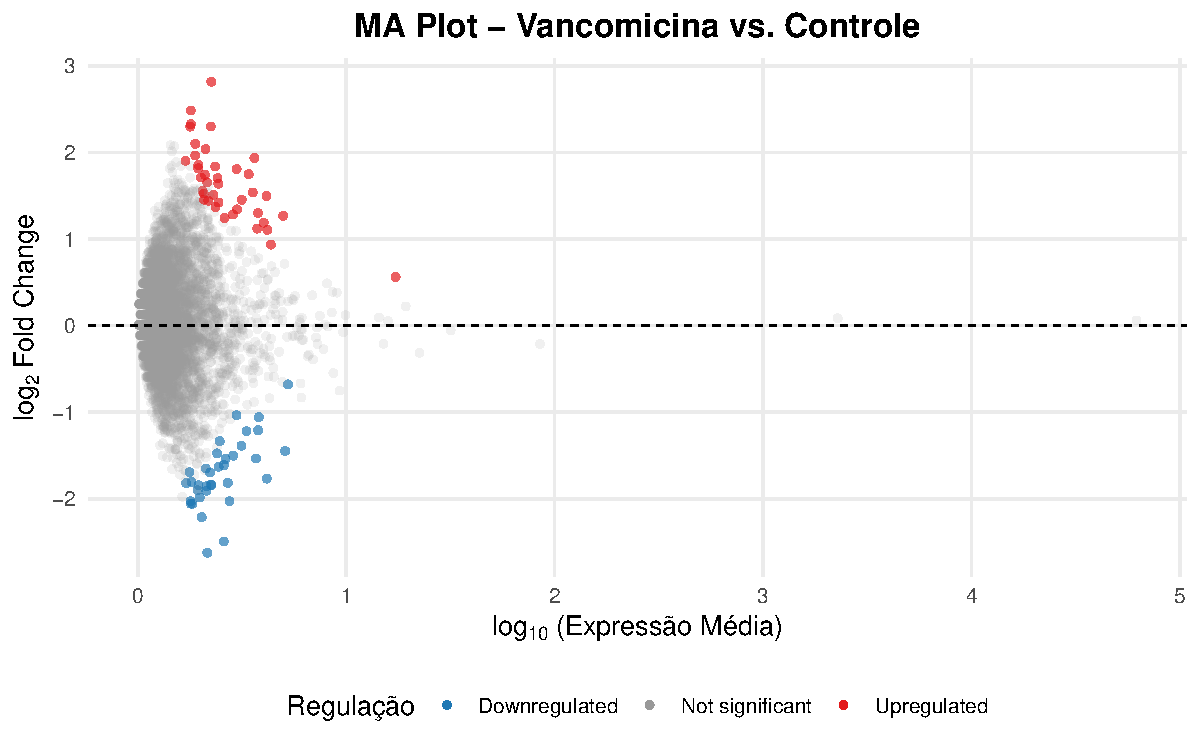
\includegraphics[keepaspectratio]{analysis/03_differential_expression_files/figure-pdf/unnamed-chunk-17-1.pdf}}

\subsubsection{Como interpretar o MA
Plot:}\label{como-interpretar-o-ma-plot}

\begin{itemize}
\tightlist
\item
  Genes à \textbf{esquerda} (baixo baseMean) possuem baixa expressão.
  Mudanças grandes nesse intervalo devem ser interpretadas com cautela,
  pois a incerteza estatística é alta.
\item
  Genes \textbf{significativos} (coloridos) que se afastam da linha
  central (log2FC = 0) são os que realmente mudaram de expressão entre
  as condições.
\item
  O ideal é que a nuvem de pontos cinza esteja \textbf{centralizada em
  zero}, indicando que a normalização foi adequada.
\end{itemize}

\subsection{14. Volcano Plot}\label{volcano-plot}

O \textbf{Volcano Plot} é o gráfico mais utilizado para visualizar
resultados de expressão diferencial. Ele combina a \textbf{significância
estatística} (-log10 do p-valor ajustado, eixo Y) com a
\textbf{magnitude da mudança} (log2FC, eixo X), permitindo identificar
rapidamente os genes mais relevantes.

\begin{Shaded}
\begin{Highlighting}[]
\FunctionTok{library}\NormalTok{(ggrepel)}

\NormalTok{padj\_cutoff }\OtherTok{\textless{}{-}} \FloatTok{0.1}  \CommentTok{\# Limiar didático (em pesquisa, use 0.05)}

\CommentTok{\# Selecionar os top 10 genes mais significativos para rotular}
\NormalTok{genes\_to\_label }\OtherTok{\textless{}{-}}\NormalTok{ res\_dge }\SpecialCharTok{\%\textgreater{}\%}
  \FunctionTok{filter}\NormalTok{(signif }\SpecialCharTok{!=} \StringTok{"Not significant"}\NormalTok{) }\SpecialCharTok{\%\textgreater{}\%}
  \FunctionTok{arrange}\NormalTok{(padj) }\SpecialCharTok{\%\textgreater{}\%}
  \FunctionTok{head}\NormalTok{(}\DecValTok{10}\NormalTok{)}

\FunctionTok{ggplot}\NormalTok{(res\_dge, }\FunctionTok{aes}\NormalTok{(}\AttributeTok{x =}\NormalTok{ log2FoldChange, }\AttributeTok{y =} \SpecialCharTok{{-}}\FunctionTok{log10}\NormalTok{(padj), }\AttributeTok{color =}\NormalTok{ signif)) }\SpecialCharTok{+}
  \FunctionTok{geom\_point}\NormalTok{(}\FunctionTok{aes}\NormalTok{(}\AttributeTok{alpha =}\NormalTok{ signif), }\AttributeTok{size =} \FloatTok{1.5}\NormalTok{) }\SpecialCharTok{+}
  \FunctionTok{scale\_color\_manual}\NormalTok{(}
    \AttributeTok{values =} \FunctionTok{c}\NormalTok{(}\StringTok{"Downregulated"} \OtherTok{=} \StringTok{"\#1F78B4"}\NormalTok{,}
               \StringTok{"Not significant"} \OtherTok{=} \StringTok{"grey60"}\NormalTok{,}
               \StringTok{"Upregulated"} \OtherTok{=} \StringTok{"\#E31A1C"}\NormalTok{),}
    \AttributeTok{name =} \StringTok{"Regulação"}
\NormalTok{  ) }\SpecialCharTok{+}
  \FunctionTok{scale\_alpha\_manual}\NormalTok{(}
    \AttributeTok{values =} \FunctionTok{c}\NormalTok{(}\StringTok{"Downregulated"} \OtherTok{=} \FloatTok{0.8}\NormalTok{,}
               \StringTok{"Not significant"} \OtherTok{=} \FloatTok{0.2}\NormalTok{,}
               \StringTok{"Upregulated"} \OtherTok{=} \FloatTok{0.8}\NormalTok{),}
    \AttributeTok{guide =} \StringTok{"none"}
\NormalTok{  ) }\SpecialCharTok{+}
  \FunctionTok{geom\_hline}\NormalTok{(}\AttributeTok{yintercept =} \SpecialCharTok{{-}}\FunctionTok{log10}\NormalTok{(padj\_cutoff),}
             \AttributeTok{linetype =} \StringTok{"dashed"}\NormalTok{, }\AttributeTok{color =} \StringTok{"black"}\NormalTok{, }\AttributeTok{linewidth =} \FloatTok{0.4}\NormalTok{) }\SpecialCharTok{+}
  \FunctionTok{geom\_text\_repel}\NormalTok{(}
    \AttributeTok{data =}\NormalTok{ genes\_to\_label,}
    \FunctionTok{aes}\NormalTok{(}\AttributeTok{label =} \FunctionTok{rownames}\NormalTok{(genes\_to\_label)),}
    \AttributeTok{size =} \DecValTok{3}\NormalTok{,}
    \AttributeTok{box.padding =} \FloatTok{0.5}\NormalTok{,}
    \AttributeTok{point.padding =} \FloatTok{0.3}\NormalTok{,}
    \AttributeTok{max.overlaps =} \ConstantTok{Inf}\NormalTok{,}
    \AttributeTok{segment.color =} \StringTok{"grey50"}\NormalTok{,}
    \AttributeTok{color =} \StringTok{"gray9"}
\NormalTok{  ) }\SpecialCharTok{+}
  \FunctionTok{labs}\NormalTok{(}
    \AttributeTok{title =} \StringTok{"Volcano Plot — Vancomicina vs. Controle (C. albicans)"}\NormalTok{,}
    \AttributeTok{x =} \FunctionTok{expression}\NormalTok{(log[}\DecValTok{2}\NormalTok{] }\SpecialCharTok{\textasciitilde{}} \StringTok{"Fold Change"}\NormalTok{),}
    \AttributeTok{y =} \FunctionTok{expression}\NormalTok{(}\StringTok{"{-}"} \SpecialCharTok{\textasciitilde{}}\NormalTok{ log[}\DecValTok{10}\NormalTok{] }\SpecialCharTok{\textasciitilde{}} \StringTok{"p{-}valor ajustado"}\NormalTok{),}
    \AttributeTok{caption =} \FunctionTok{paste0}\NormalTok{(}\StringTok{"Cutoff: padj \textless{} "}\NormalTok{, padj\_cutoff)}
\NormalTok{  ) }\SpecialCharTok{+}
  \FunctionTok{theme\_minimal}\NormalTok{(}\AttributeTok{base\_size =} \DecValTok{13}\NormalTok{) }\SpecialCharTok{+}
  \FunctionTok{theme}\NormalTok{(}
    \AttributeTok{plot.title =} \FunctionTok{element\_text}\NormalTok{(}\AttributeTok{hjust =} \FloatTok{0.5}\NormalTok{, }\AttributeTok{face =} \StringTok{"bold"}\NormalTok{),}
    \AttributeTok{legend.position =} \StringTok{"bottom"}\NormalTok{,}
    \AttributeTok{panel.grid.minor =} \FunctionTok{element\_blank}\NormalTok{(),}
    \AttributeTok{panel.background =} \FunctionTok{element\_rect}\NormalTok{(}\AttributeTok{fill =} \StringTok{"white"}\NormalTok{, }\AttributeTok{color =} \ConstantTok{NA}\NormalTok{),}
    \AttributeTok{plot.background =} \FunctionTok{element\_rect}\NormalTok{(}\AttributeTok{fill =} \StringTok{"white"}\NormalTok{, }\AttributeTok{color =} \ConstantTok{NA}\NormalTok{)}
\NormalTok{  )}
\end{Highlighting}
\end{Shaded}

\pandocbounded{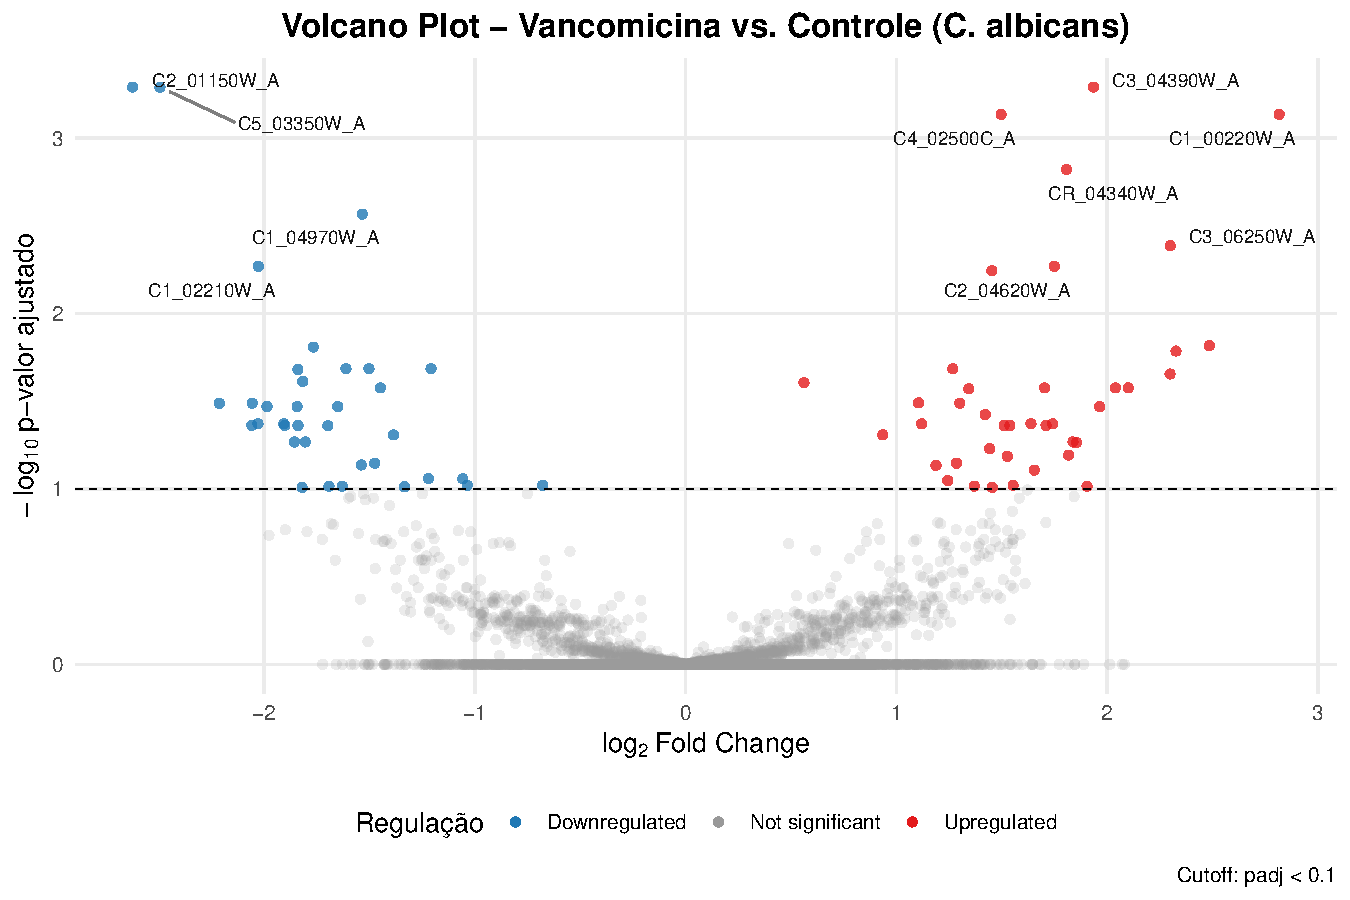
\includegraphics[keepaspectratio]{analysis/03_differential_expression_files/figure-pdf/unnamed-chunk-18-1.pdf}}

\subsubsection{Como interpretar o Volcano
Plot:}\label{como-interpretar-o-volcano-plot}

\begin{itemize}
\tightlist
\item
  \textbf{Eixo X (log2FC)}: genes à direita estão upregulados sob o
  tratamento de vancomicina; genes à esquerda estão downregulados.
\item
  \textbf{Eixo Y (-log10 padj)}: quanto mais alto o ponto, mais
  significativa é a mudança. A linha tracejada marca o threshold de padj
  = 0.1.
\item
  Os \textbf{genes rotulados} são os top 10 mais significativos.
\end{itemize}

\begin{tcolorbox}[enhanced jigsaw, arc=.35mm, bottomrule=.15mm, bottomtitle=1mm, breakable, colback=white, colbacktitle=quarto-callout-tip-color!10!white, colframe=quarto-callout-tip-color-frame, coltitle=black, left=2mm, leftrule=.75mm, opacityback=0, opacitybacktitle=0.6, rightrule=.15mm, title=\textcolor{quarto-callout-tip-color}{\faLightbulb}\hspace{0.5em}{O que o Volcano Plot nos diz biologicamente?}, titlerule=0mm, toprule=.15mm, toptitle=1mm]

Observe a distribuição entre upregulados e downregulados. Se o
tratamento com vancomicina remodela a resposta transcricional da
\emph{Candida}, esperamos ver genes envolvidos em \textbf{resistência a
estresse}, \textbf{remodelamento da parede celular} e
\textbf{virulência} entre os mais significativos. Genes de
\emph{housekeeping} devem permanecer na região cinza central.

\end{tcolorbox}

\subsection{15. Heatmap dos Genes Diferencialmente
Expressos}\label{heatmap-dos-genes-diferencialmente-expressos}

O \textbf{heatmap} nos permite visualizar o padrão de expressão dos
genes significativos em todas as amostras simultaneamente. Para isso,
utilizamos os valores de expressão normalizados transformados em
\textbf{z-score} (escala por gene), o que evidencia as diferenças
relativas entre condições.

\begin{Shaded}
\begin{Highlighting}[]
\CommentTok{\# Filtrar apenas os genes significativos (padj \textless{}= 0.05)}
\NormalTok{res\_dge\_signif }\OtherTok{\textless{}{-}} \FunctionTok{subset}\NormalTok{(res\_dge, padj }\SpecialCharTok{\textless{}=} \FloatTok{0.05}\NormalTok{)}

\CommentTok{\# Obter contagens normalizadas}
\NormalTok{exp\_genes }\OtherTok{\textless{}{-}}\NormalTok{ DESeq2}\SpecialCharTok{::}\FunctionTok{counts}\NormalTok{(dds, }\AttributeTok{normalized =} \ConstantTok{TRUE}\NormalTok{)}

\CommentTok{\# Selecionar apenas os genes DEG}
\NormalTok{idx }\OtherTok{\textless{}{-}} \FunctionTok{rownames}\NormalTok{(exp\_genes) }\SpecialCharTok{\%in\%} \FunctionTok{rownames}\NormalTok{(res\_dge\_signif)}
\NormalTok{exp\_dge }\OtherTok{\textless{}{-}}\NormalTok{ exp\_genes[idx, ]}

\CommentTok{\# Transformar em z{-}score (por gene)}
\NormalTok{exp\_dge\_z }\OtherTok{\textless{}{-}} \FunctionTok{t}\NormalTok{(}\FunctionTok{apply}\NormalTok{(exp\_dge, }\DecValTok{1}\NormalTok{, scale, }\AttributeTok{center =} \ConstantTok{TRUE}\NormalTok{, }\AttributeTok{scale =} \ConstantTok{TRUE}\NormalTok{))}
\FunctionTok{colnames}\NormalTok{(exp\_dge\_z) }\OtherTok{\textless{}{-}} \FunctionTok{colnames}\NormalTok{(exp\_dge)}

\CommentTok{\# Criar anotação das colunas}
\NormalTok{ann\_col }\OtherTok{\textless{}{-}} \FunctionTok{data.frame}\NormalTok{(}
  \AttributeTok{Tratamento =}\NormalTok{ metadata}\SpecialCharTok{$}\NormalTok{treatment,}
  \AttributeTok{Lote =}\NormalTok{ metadata}\SpecialCharTok{$}\NormalTok{experiment\_group,}
  \AttributeTok{row.names =} \FunctionTok{rownames}\NormalTok{(metadata)}
\NormalTok{)}

\NormalTok{ann\_colors }\OtherTok{\textless{}{-}} \FunctionTok{list}\NormalTok{(}
  \AttributeTok{Tratamento =} \FunctionTok{c}\NormalTok{(}\StringTok{"Untreated (control)"} \OtherTok{=} \StringTok{"\#4393C3"}\NormalTok{, }\StringTok{"Vancomycin"} \OtherTok{=} \StringTok{"\#D6604D"}\NormalTok{),}
  \AttributeTok{Lote =} \FunctionTok{c}\NormalTok{(}\StringTok{"1"} \OtherTok{=} \StringTok{"\#F0E442"}\NormalTok{, }\StringTok{"2"} \OtherTok{=} \StringTok{"\#E69F00"}\NormalTok{, }\StringTok{"3"} \OtherTok{=} \StringTok{"\#56B4E9"}\NormalTok{,}
           \StringTok{"4"} \OtherTok{=} \StringTok{"\#009E73"}\NormalTok{, }\StringTok{"5"} \OtherTok{=} \StringTok{"\#CC79A7"}\NormalTok{, }\StringTok{"6"} \OtherTok{=} \StringTok{"\#999999"}\NormalTok{)}
\NormalTok{)}

\CommentTok{\# Plotar heatmap}
\FunctionTok{pheatmap}\NormalTok{(exp\_dge\_z,}
         \AttributeTok{show\_rownames =} \ConstantTok{FALSE}\NormalTok{,}
         \AttributeTok{annotation\_col =}\NormalTok{ ann\_col,}
         \AttributeTok{annotation\_colors =}\NormalTok{ ann\_colors,}
         \AttributeTok{cluster\_cols =} \ConstantTok{TRUE}\NormalTok{,}
         \AttributeTok{fontsize =} \DecValTok{9}\NormalTok{,}
         \AttributeTok{main =} \StringTok{"Heatmap — Genes Diferencialmente Expressos (z{-}score)"}\NormalTok{)}
\end{Highlighting}
\end{Shaded}

\pandocbounded{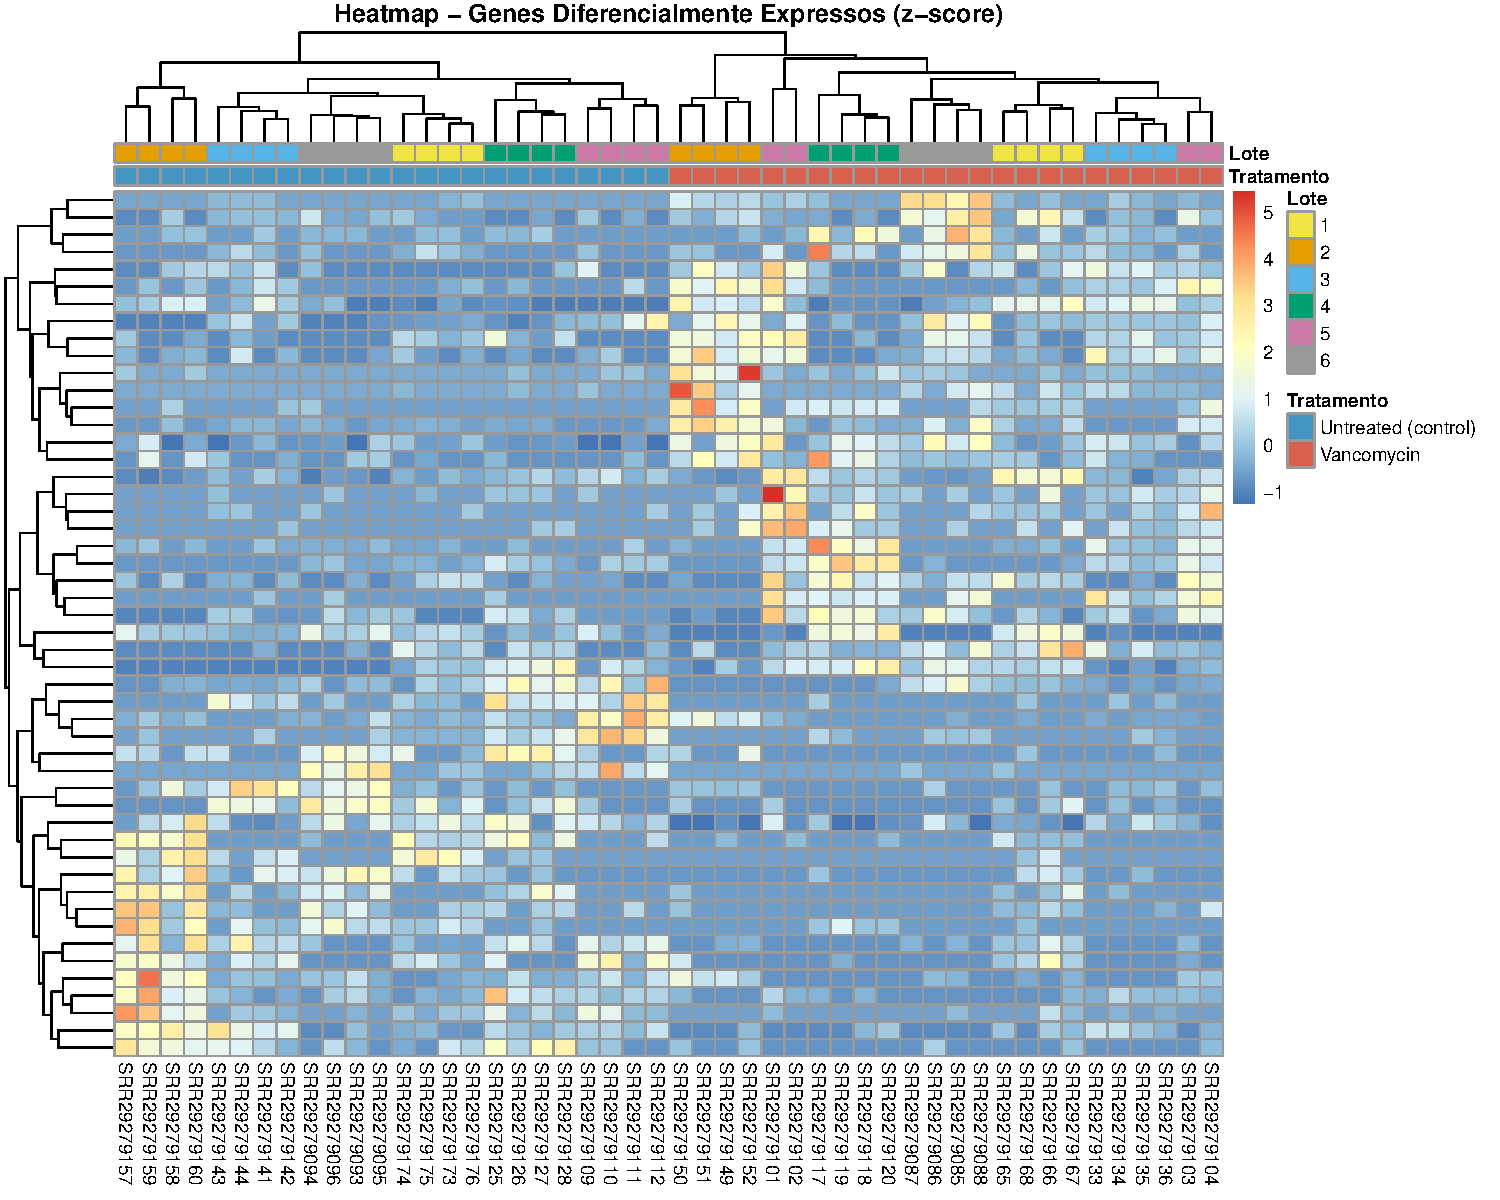
\includegraphics[keepaspectratio]{analysis/03_differential_expression_files/figure-pdf/unnamed-chunk-19-1.pdf}}

\subsubsection{Como interpretar o
heatmap:}\label{como-interpretar-o-heatmap}

\begin{itemize}
\tightlist
\item
  Cada \textbf{linha} é um gene diferencialmente expresso e cada
  \textbf{coluna} é uma amostra.
\item
  As \textbf{cores} representam o z-score: \textbf{vermelho} indica
  expressão acima da média daquele gene, enquanto \textbf{azul} indica
  expressão abaixo da média.
\item
  A \textbf{barra de anotação superior} diferencia as amostras por
  tratamento e lote.
\item
  Se os genes DEG segregam perfeitamente as amostras por tratamento,
  isso confirma que o sinal biológico é forte e consistente entre os
  lotes.
\item
  Note que as \textbf{linhas são clusterizadas}: genes com padrões de
  expressão similares ficam próximos, revelando blocos de genes
  co-regulados.
\end{itemize}

\begin{Shaded}
\begin{Highlighting}[]
\CommentTok{\# Salvar a tabela de genes diferencialmente expressos para a próxima etapa}
\FunctionTok{saveRDS}\NormalTok{(res\_dge, }\AttributeTok{file =}\NormalTok{ here}\SpecialCharTok{::}\FunctionTok{here}\NormalTok{(}\StringTok{"data/DGE/res\_dge.rds"}\NormalTok{))}
\end{Highlighting}
\end{Shaded}

\begin{center}\rule{0.5\linewidth}{0.5pt}\end{center}

\textbf{Identificamos os genes da \emph{Candida albicans} cuja expressão
mudou significativamente em resposta à vancomicina. Mas o que esses
genes fazem? A quais vias biológicas eles pertencem? Essas perguntas
serão respondidas na próxima seção, onde realizaremos a análise de
enriquecimento funcional.}

\bookmarksetup{startatroot}

\chapter{Análises Downstream}\label{anuxe1lises-downstream}

Na etapa anterior, identificamos quais genes da \emph{Candida albicans}
tiveram sua expressão significativamente alterada pelo tratamento com
vancomicina. Mas uma lista de genes, por si só, diz pouco sobre a
biologia do organismo. Para extrairmos significado biológico, precisamos
perguntar: \textbf{esses genes pertencem a vias biológicas específicas?
Há processos celulares mais afetados do que o esperado ao acaso?}

É exatamente isso que a \textbf{análise de enriquecimento funcional} nos
permite responder.

\begin{center}\rule{0.5\linewidth}{0.5pt}\end{center}

\bookmarksetup{startatroot}

\chapter{Enriquecimento Funcional}\label{enriquecimento-funcional}

A análise de enriquecimento funcional verifica se, entre os genes
diferencialmente expressos, há um número desproporcional de genes
pertencentes a uma determinada via biológica ou processo celular. Se
encontrarmos mais genes alterados em uma via do que o esperado por
acaso, dizemos que essa via está \textbf{enriquecida}.

A abordagem que utilizaremos é a \textbf{ORA (Over-Representation
Analysis)}, que parte da nossa lista de genes significativos e aplica um
teste hipergeométrico para verificar quais vias estão
sobre-representadas. Para os bancos de dados, utilizaremos o
\textbf{KEGG Pathways} e o \textbf{Gene Ontology (GO)}.

\section{O que são GO e KEGG?}\label{o-que-suxe3o-go-e-kegg}

\subsection{Gene Ontology (GO)}\label{gene-ontology-go}

O \href{http://geneontology.org/}{Gene Ontology} é um sistema de
ontologias que descreve a função dos genes em três dimensões
independentes (ontologias):

\begin{itemize}
\tightlist
\item
  \textbf{Biological Process (BP)}: o processo celular de que o gene
  participa (ex: \emph{resposta a estresse oxidativo}, \emph{biossíntese
  da parede celular}).
\item
  \textbf{Molecular Function (MF)}: a atividade molecular que a proteína
  exerce (ex: \emph{atividade de quinase}, \emph{ligação a ATP}).
\item
  \textbf{Cellular Component (CC)}: onde no espaço celular a proteína
  atua (ex: \emph{núcleo}, \emph{membrana plasmática}).
\end{itemize}

A GO é organizada como um \textbf{grafo acíclico dirigido (DAG)}: termos
mais gerais (ex: \emph{processo metabólico}) estão no topo da
hierarquia, e termos mais específicos (ex: \emph{biossíntese de
ergosterol}) estão na base. Um gene pode ser anotado em múltiplos termos
e em múltiplas ontologias simultaneamente.

\subsection{KEGG Pathways}\label{kegg-pathways}

O \href{https://www.kegg.jp/}{KEGG (Kyoto Encyclopedia of Genes and
Genomes)} é um banco de dados que organiza o conhecimento biológico em
\textbf{mapas de vias metabólicas e de sinalização}. Cada via é um
diagrama que conecta enzimas, metabólitos e reações em sequência,
representando processos como a glicólise, o ciclo do TCA ou a
biossíntese de aminoácidos.

Diferente do GO, o KEGG tem uma estrutura \textbf{plana} (não
hierárquica): cada via é independente e autocontida. Além disso, o KEGG
inclui informações sobre \textbf{reações bioquímicas} e
\textbf{compostos químicos}, o que o torna especialmente útil para
estudar metabolismo.

\subsection{Principais diferenças}\label{principais-diferenuxe7as}

{\def\LTcaptype{none} % do not increment counter
\begin{longtable}[]{@{}
  >{\raggedright\arraybackslash}p{(\linewidth - 4\tabcolsep) * \real{0.3333}}
  >{\raggedright\arraybackslash}p{(\linewidth - 4\tabcolsep) * \real{0.3333}}
  >{\raggedright\arraybackslash}p{(\linewidth - 4\tabcolsep) * \real{0.3333}}@{}}
\toprule\noalign{}
\begin{minipage}[b]{\linewidth}\raggedright
Característica
\end{minipage} & \begin{minipage}[b]{\linewidth}\raggedright
Gene Ontology (GO)
\end{minipage} & \begin{minipage}[b]{\linewidth}\raggedright
KEGG Pathways
\end{minipage} \\
\midrule\noalign{}
\endhead
\bottomrule\noalign{}
\endlastfoot
\textbf{Estrutura} & Hierárquica (DAG) & Plana (mapas independentes) \\
\textbf{Foco} & Funções, processos e localização & Vias metabólicas e de
sinalização \\
\textbf{Granularidade} & Alta (termos muito específicos a gerais) &
Moderada (vias completas) \\
\textbf{Curadoria} & Comunidade científica global & Equipe centralizada
(Kanehisa Lab) \\
\textbf{Organismo} & Ampla cobertura (via OrgDb ou GAF) & Código por
organismo (ex: \texttt{cal}) \\
\end{longtable}
}

\section{A Importância dos Bancos de Dados
Curados}\label{a-importuxe2ncia-dos-bancos-de-dados-curados}

Antes de começar, é fundamental entender que \textbf{o enriquecimento
funcional depende inteiramente da qualidade e completude das anotações
disponíveis para o organismo estudado}. Para organismos-modelo como
\emph{Homo sapiens} ou \emph{Mus musculus}, bancos como KEGG, Gene
Ontology e Reactome possuem anotações extensas, curadas por décadas de
pesquisa. O resultado é que milhares de genes estão anotados em centenas
de vias biológicas, e o teste estatístico tem alta chance de encontrar
padrões significativos.

Para organismos não-modelo como \emph{Candida albicans}, a situação é
diferente:

\begin{itemize}
\tightlist
\item
  \textbf{Menos genes anotados}: uma fração menor do genoma possui
  anotação funcional.
\item
  \textbf{Menos vias catalogadas}: o número de vias biológicas mapeadas
  é mais restrito.
\item
  \textbf{Anotações menos curadas}: muitas anotações são inferidas
  computacionalmente (IEA - \emph{Inferred from Electronic Annotation}),
  e não por evidência experimental direta.
\end{itemize}

Isso significa que, mesmo que nossos genes estejam participando de
processos biológicos relevantes, \textbf{se esses processos não
estiverem adequadamente anotados no banco de dados, o enriquecimento
simplesmente não os detectará}. Por isso, para \emph{C. albicans},
utilizaremos tanto o KEGG (que suporta o organismo nativamente) quanto
as anotações curadas do \textbf{Candida Genome Database (CGD)}, o banco
de referência para genômica de \emph{Candida}, que possui mais de 33 mil
anotações GO específicas.

\begin{tcolorbox}[enhanced jigsaw, arc=.35mm, bottomrule=.15mm, bottomtitle=1mm, breakable, colback=white, colbacktitle=quarto-callout-warning-color!10!white, colframe=quarto-callout-warning-color-frame, coltitle=black, left=2mm, leftrule=.75mm, opacityback=0, opacitybacktitle=0.6, rightrule=.15mm, title=\textcolor{quarto-callout-warning-color}{\faExclamationTriangle}\hspace{0.5em}{Nota Didática --- Thresholds Relaxados}, titlerule=0mm, toprule=.15mm, toptitle=1mm]

Em publicações científicas, os cortes padrão para enriquecimento são
\textbf{p.adjust ≤ 0.05} e \textbf{qvalue ≤ 0.05}. Neste minicurso,
utilizamos thresholds mais permissivos (\textbf{p.adjust ≤ 0.5} e
\textbf{qvalue ≤ 0.5}) para fins \textbf{didáticos}, de modo que seja
possível visualizar e interpretar os gráficos de enriquecimento mesmo
com um número reduzido de DEGs. Em um cenário de pesquisa real,
recomendamos utilizar os cortes padrão.

\end{tcolorbox}

\section{1. Carregando os Pacotes}\label{carregando-os-pacotes-1}

\begin{Shaded}
\begin{Highlighting}[]
\FunctionTok{suppressPackageStartupMessages}\NormalTok{(\{}
  \FunctionTok{library}\NormalTok{(clusterProfiler)}
  \FunctionTok{library}\NormalTok{(KEGGREST)}
  \FunctionTok{library}\NormalTok{(enrichplot)}
  \FunctionTok{library}\NormalTok{(GO.db)}
  \FunctionTok{library}\NormalTok{(dplyr)}
  \FunctionTok{library}\NormalTok{(readr)}
  \FunctionTok{library}\NormalTok{(tibble)}
  \FunctionTok{library}\NormalTok{(ggplot2)}
\NormalTok{\})}
\end{Highlighting}
\end{Shaded}

\section{2. Carregando os Resultados da Expressão
Diferencial}\label{carregando-os-resultados-da-expressuxe3o-diferencial}

Vamos recuperar a tabela de resultados que salvamos no módulo anterior:

\begin{Shaded}
\begin{Highlighting}[]
\NormalTok{res\_dge }\OtherTok{\textless{}{-}} \FunctionTok{readRDS}\NormalTok{(here}\SpecialCharTok{::}\FunctionTok{here}\NormalTok{(}\StringTok{"data/DGE/res\_dge.rds"}\NormalTok{))}

\FunctionTok{head}\NormalTok{(res\_dge)}
\end{Highlighting}
\end{Shaded}

\begin{verbatim}
              baseMean log2FoldChange     lfcSE        stat    pvalue      padj
C1_00010W_A 0.13073479      0.2439030 2.5493706  0.09567186 0.9237812 1.0000000
C1_00020C_A 1.35871278     -0.7858614 0.5442897 -1.44382928 0.1487870 0.5357854
C1_00030C_A 0.02292633      0.2485875 2.9448570  0.08441413 0.9327272 1.0000000
C1_00040W_A 0.03442856      0.3688108 2.9448570  0.12523896 0.9003344 1.0000000
C1_00050C_A 0.03644129     -0.1120823 2.9448570 -0.03806036 0.9696396 1.0000000
C1_00060W_A 0.36778762      0.4121354 1.3458047  0.30623715 0.7594241 1.0000000
                     signif
C1_00010W_A Not significant
C1_00020C_A Not significant
C1_00030C_A Not significant
C1_00040W_A Not significant
C1_00050C_A Not significant
C1_00060W_A Not significant
\end{verbatim}

\section{3. Preparando os Conjuntos de
Genes}\label{preparando-os-conjuntos-de-genes}

Vamos preparar três conjuntos de genes para o enriquecimento: os
\textbf{upregulados}, os \textbf{downregulados} e \textbf{todos os DEGs}
juntos.

\begin{Shaded}
\begin{Highlighting}[]
\NormalTok{genes\_up }\OtherTok{\textless{}{-}} \FunctionTok{rownames}\NormalTok{(}\FunctionTok{subset}\NormalTok{(res\_dge, signif }\SpecialCharTok{==} \StringTok{"Upregulated"}\NormalTok{))}
\NormalTok{genes\_down }\OtherTok{\textless{}{-}} \FunctionTok{rownames}\NormalTok{(}\FunctionTok{subset}\NormalTok{(res\_dge, signif }\SpecialCharTok{==} \StringTok{"Downregulated"}\NormalTok{))}
\NormalTok{genes\_all }\OtherTok{\textless{}{-}} \FunctionTok{rownames}\NormalTok{(}\FunctionTok{subset}\NormalTok{(res\_dge, signif }\SpecialCharTok{!=} \StringTok{"Not significant"}\NormalTok{))}

\FunctionTok{cat}\NormalTok{(}\StringTok{"Genes upregulados:"}\NormalTok{, }\FunctionTok{length}\NormalTok{(genes\_up), }\StringTok{"}\SpecialCharTok{\textbackslash{}n}\StringTok{"}\NormalTok{)}
\end{Highlighting}
\end{Shaded}

\begin{verbatim}
Genes upregulados: 40 
\end{verbatim}

\begin{Shaded}
\begin{Highlighting}[]
\FunctionTok{cat}\NormalTok{(}\StringTok{"Genes downregulados:"}\NormalTok{, }\FunctionTok{length}\NormalTok{(genes\_down), }\StringTok{"}\SpecialCharTok{\textbackslash{}n}\StringTok{"}\NormalTok{)}
\end{Highlighting}
\end{Shaded}

\begin{verbatim}
Genes downregulados: 35 
\end{verbatim}

\begin{Shaded}
\begin{Highlighting}[]
\FunctionTok{cat}\NormalTok{(}\StringTok{"Total DEGs:"}\NormalTok{, }\FunctionTok{length}\NormalTok{(genes\_all), }\StringTok{"}\SpecialCharTok{\textbackslash{}n}\StringTok{"}\NormalTok{)}
\end{Highlighting}
\end{Shaded}

\begin{verbatim}
Total DEGs: 75 
\end{verbatim}

\begin{center}\rule{0.5\linewidth}{0.5pt}\end{center}

\section{4. Conversão de Identificadores para o
KEGG}\label{conversuxe3o-de-identificadores-para-o-kegg}

Os nossos identificadores de genes seguem o padrão do Ensembl Fungi (ex:
\texttt{C1\_00010W\_A}), mas o KEGG utiliza um formato próprio para
\emph{C. albicans} (ex: \texttt{CAALFM\_C100010WA}). Precisamos
construir o dicionário para conversão:

\begin{Shaded}
\begin{Highlighting}[]
\CommentTok{\# Baixar todos os genes de C. albicans (cal) do KEGG}
\NormalTok{kegg\_genes }\OtherTok{\textless{}{-}} \FunctionTok{keggList}\NormalTok{(}\StringTok{"cal"}\NormalTok{)}

\CommentTok{\# Criar tabela de mapeamento}
\NormalTok{kegg\_mapping }\OtherTok{\textless{}{-}} \FunctionTok{data.frame}\NormalTok{(}
  \AttributeTok{kegg\_id =} \FunctionTok{sub}\NormalTok{(}\StringTok{"cal:"}\NormalTok{, }\StringTok{""}\NormalTok{, }\FunctionTok{names}\NormalTok{(kegg\_genes)),}
  \AttributeTok{description =} \FunctionTok{as.character}\NormalTok{(kegg\_genes),}
  \AttributeTok{stringsAsFactors =} \ConstantTok{FALSE}
\NormalTok{)}

\CommentTok{\# Gerar o ID Ensembl Fungi equivalente a partir do KEGG ID}
\NormalTok{kegg\_mapping }\OtherTok{\textless{}{-}}\NormalTok{ kegg\_mapping }\SpecialCharTok{\%\textgreater{}\%}
  \FunctionTok{mutate}\NormalTok{(}
    \AttributeTok{core =} \FunctionTok{sub}\NormalTok{(}\StringTok{"\^{}CAALFM\_"}\NormalTok{, }\StringTok{""}\NormalTok{, kegg\_id),}
    \AttributeTok{ensembl\_id =} \FunctionTok{gsub}\NormalTok{(}
      \StringTok{"\^{}(C[0{-}9R]+)(}\SpecialCharTok{\textbackslash{}\textbackslash{}}\StringTok{d\{5\})(}\SpecialCharTok{\textbackslash{}\textbackslash{}}\StringTok{w)(}\SpecialCharTok{\textbackslash{}\textbackslash{}}\StringTok{w)$"}\NormalTok{,}
      \StringTok{"}\SpecialCharTok{\textbackslash{}\textbackslash{}}\StringTok{1\_}\SpecialCharTok{\textbackslash{}\textbackslash{}}\StringTok{2}\SpecialCharTok{\textbackslash{}\textbackslash{}}\StringTok{3\_}\SpecialCharTok{\textbackslash{}\textbackslash{}}\StringTok{4"}\NormalTok{,}
\NormalTok{      core}
\NormalTok{    )}
\NormalTok{  )}

\CommentTok{\# Verificar quantos dos nossos genes têm correspondência}
\NormalTok{genes\_com\_kegg }\OtherTok{\textless{}{-}} \FunctionTok{sum}\NormalTok{(}\FunctionTok{rownames}\NormalTok{(res\_dge) }\SpecialCharTok{\%in\%}\NormalTok{ kegg\_mapping}\SpecialCharTok{$}\NormalTok{ensembl\_id)}
\FunctionTok{cat}\NormalTok{(}\StringTok{"Genes mapeados para KEGG:"}\NormalTok{, genes\_com\_kegg, }\StringTok{"de"}\NormalTok{, }\FunctionTok{nrow}\NormalTok{(res\_dge), }\StringTok{"}\SpecialCharTok{\textbackslash{}n}\StringTok{"}\NormalTok{)}
\end{Highlighting}
\end{Shaded}

\begin{verbatim}
Genes mapeados para KEGG: 6117 de 6468 
\end{verbatim}

\begin{Shaded}
\begin{Highlighting}[]
\CommentTok{\# Criar dicionário: Ensembl → KEGG}
\NormalTok{ensembl\_to\_kegg }\OtherTok{\textless{}{-}} \FunctionTok{setNames}\NormalTok{(kegg\_mapping}\SpecialCharTok{$}\NormalTok{kegg\_id, kegg\_mapping}\SpecialCharTok{$}\NormalTok{ensembl\_id)}

\CommentTok{\# Converter cada conjunto de genes}
\NormalTok{genes\_up\_kegg }\OtherTok{\textless{}{-}} \FunctionTok{unname}\NormalTok{(ensembl\_to\_kegg[genes\_up[genes\_up }\SpecialCharTok{\%in\%} \FunctionTok{names}\NormalTok{(ensembl\_to\_kegg)]])}
\NormalTok{genes\_down\_kegg }\OtherTok{\textless{}{-}} \FunctionTok{unname}\NormalTok{(ensembl\_to\_kegg[genes\_down[genes\_down }\SpecialCharTok{\%in\%} \FunctionTok{names}\NormalTok{(ensembl\_to\_kegg)]])}
\NormalTok{genes\_all\_kegg }\OtherTok{\textless{}{-}} \FunctionTok{unname}\NormalTok{(ensembl\_to\_kegg[genes\_all[genes\_all }\SpecialCharTok{\%in\%} \FunctionTok{names}\NormalTok{(ensembl\_to\_kegg)]])}

\FunctionTok{cat}\NormalTok{(}\StringTok{"UP com KEGG ID:"}\NormalTok{, }\FunctionTok{length}\NormalTok{(genes\_up\_kegg), }\StringTok{"}\SpecialCharTok{\textbackslash{}n}\StringTok{"}\NormalTok{)}
\end{Highlighting}
\end{Shaded}

\begin{verbatim}
UP com KEGG ID: 40 
\end{verbatim}

\begin{Shaded}
\begin{Highlighting}[]
\FunctionTok{cat}\NormalTok{(}\StringTok{"DOWN com KEGG ID:"}\NormalTok{, }\FunctionTok{length}\NormalTok{(genes\_down\_kegg), }\StringTok{"}\SpecialCharTok{\textbackslash{}n}\StringTok{"}\NormalTok{)}
\end{Highlighting}
\end{Shaded}

\begin{verbatim}
DOWN com KEGG ID: 35 
\end{verbatim}

\begin{Shaded}
\begin{Highlighting}[]
\FunctionTok{cat}\NormalTok{(}\StringTok{"ALL com KEGG ID:"}\NormalTok{, }\FunctionTok{length}\NormalTok{(genes\_all\_kegg), }\StringTok{"}\SpecialCharTok{\textbackslash{}n}\StringTok{"}\NormalTok{)}
\end{Highlighting}
\end{Shaded}

\begin{verbatim}
ALL com KEGG ID: 75 
\end{verbatim}

\begin{center}\rule{0.5\linewidth}{0.5pt}\end{center}

\section{5. Enriquecimento KEGG --- ORA}\label{enriquecimento-kegg-ora}

Vamos rodar a ORA com o KEGG Pathways separadamente para genes
upregulados, downregulados e todos os DEGs:

\begin{Shaded}
\begin{Highlighting}[]
\CommentTok{\# KEGG ORA — Upregulados}
\NormalTok{kegg\_up }\OtherTok{\textless{}{-}} \FunctionTok{enrichKEGG}\NormalTok{(}
  \AttributeTok{gene =}\NormalTok{ genes\_up\_kegg, }\AttributeTok{organism =} \StringTok{"cal"}\NormalTok{, }\AttributeTok{keyType =} \StringTok{"kegg"}\NormalTok{,}
  \AttributeTok{pvalueCutoff =} \FloatTok{0.5}\NormalTok{, }\AttributeTok{qvalueCutoff =} \FloatTok{0.5}\NormalTok{, }\AttributeTok{pAdjustMethod =} \StringTok{"BH"}
\NormalTok{)}

\CommentTok{\# KEGG ORA — Downregulados}
\NormalTok{kegg\_down }\OtherTok{\textless{}{-}} \FunctionTok{enrichKEGG}\NormalTok{(}
  \AttributeTok{gene =}\NormalTok{ genes\_down\_kegg, }\AttributeTok{organism =} \StringTok{"cal"}\NormalTok{, }\AttributeTok{keyType =} \StringTok{"kegg"}\NormalTok{,}
  \AttributeTok{pvalueCutoff =} \FloatTok{0.5}\NormalTok{, }\AttributeTok{qvalueCutoff =} \FloatTok{0.5}\NormalTok{, }\AttributeTok{pAdjustMethod =} \StringTok{"BH"}
\NormalTok{)}

\CommentTok{\# KEGG ORA — Todos os DEGs}
\NormalTok{kegg\_all }\OtherTok{\textless{}{-}} \FunctionTok{enrichKEGG}\NormalTok{(}
  \AttributeTok{gene =}\NormalTok{ genes\_all\_kegg, }\AttributeTok{organism =} \StringTok{"cal"}\NormalTok{, }\AttributeTok{keyType =} \StringTok{"kegg"}\NormalTok{,}
  \AttributeTok{pvalueCutoff =} \FloatTok{0.5}\NormalTok{, }\AttributeTok{qvalueCutoff =} \FloatTok{0.5}\NormalTok{, }\AttributeTok{pAdjustMethod =} \StringTok{"BH"}
\NormalTok{)}
\end{Highlighting}
\end{Shaded}

\subsection{Dotplot --- KEGG
Upregulados}\label{dotplot-kegg-upregulados}

\begin{Shaded}
\begin{Highlighting}[]
\ControlFlowTok{if}\NormalTok{ (}\SpecialCharTok{!}\FunctionTok{is.null}\NormalTok{(kegg\_up) }\SpecialCharTok{\&\&} \FunctionTok{nrow}\NormalTok{(}\FunctionTok{as.data.frame}\NormalTok{(kegg\_up)) }\SpecialCharTok{\textgreater{}} \DecValTok{0}\NormalTok{) \{}
  \FunctionTok{dotplot}\NormalTok{(kegg\_up,}
          \AttributeTok{showCategory =} \DecValTok{15}\NormalTok{,}
          \AttributeTok{title =} \StringTok{"KEGG — Genes Upregulados"}\NormalTok{,}
          \AttributeTok{color =} \StringTok{"p.adjust"}\NormalTok{) }\SpecialCharTok{+}
    \FunctionTok{theme}\NormalTok{(}\AttributeTok{axis.text.y =} \FunctionTok{element\_text}\NormalTok{(}\AttributeTok{size =} \DecValTok{10}\NormalTok{)) }\SpecialCharTok{+}
    \FunctionTok{scale\_color\_gradient}\NormalTok{(}\AttributeTok{low =} \StringTok{"\#E31A1C"}\NormalTok{, }\AttributeTok{high =} \StringTok{"\#FCBBA1"}\NormalTok{, }\AttributeTok{name =} \StringTok{"p{-}valor}\SpecialCharTok{\textbackslash{}n}\StringTok{ajustado"}\NormalTok{)}
\NormalTok{\} }\ControlFlowTok{else}\NormalTok{ \{}
  \FunctionTok{cat}\NormalTok{(}\StringTok{"Nenhuma via KEGG enriquecida para genes upregulados.}\SpecialCharTok{\textbackslash{}n}\StringTok{"}\NormalTok{)}
\NormalTok{\}}
\end{Highlighting}
\end{Shaded}

\pandocbounded{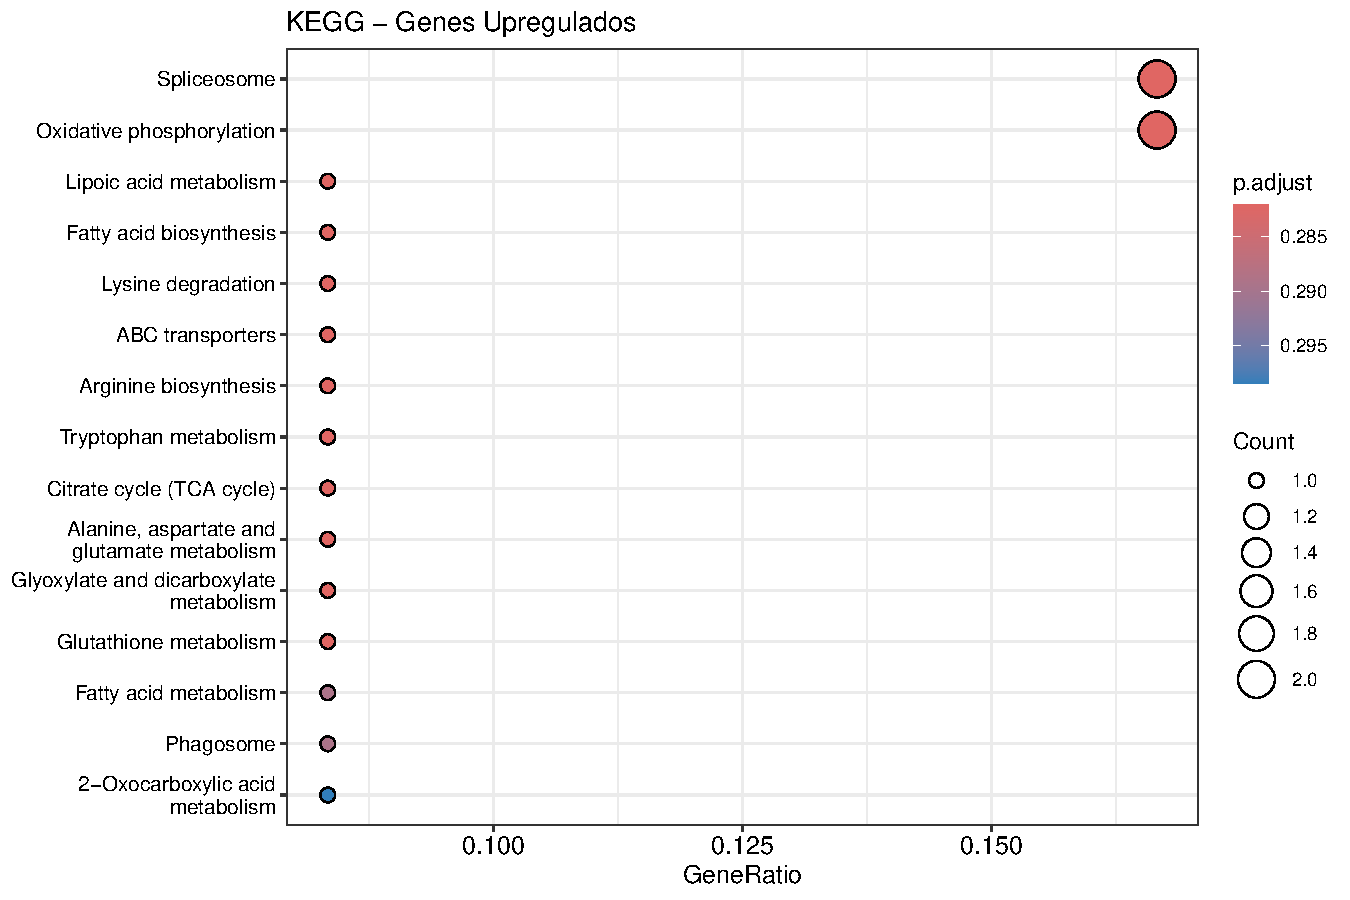
\includegraphics[keepaspectratio]{analysis/04_downstream_analyses_files/figure-pdf/unnamed-chunk-7-1.pdf}}

\subsection{Dotplot --- KEGG
Downregulados}\label{dotplot-kegg-downregulados}

\begin{Shaded}
\begin{Highlighting}[]
\ControlFlowTok{if}\NormalTok{ (}\SpecialCharTok{!}\FunctionTok{is.null}\NormalTok{(kegg\_down) }\SpecialCharTok{\&\&} \FunctionTok{nrow}\NormalTok{(}\FunctionTok{as.data.frame}\NormalTok{(kegg\_down)) }\SpecialCharTok{\textgreater{}} \DecValTok{0}\NormalTok{) \{}
  \FunctionTok{dotplot}\NormalTok{(kegg\_down,}
          \AttributeTok{showCategory =} \DecValTok{15}\NormalTok{,}
          \AttributeTok{title =} \StringTok{"KEGG — Genes Downregulados"}\NormalTok{,}
          \AttributeTok{color =} \StringTok{"p.adjust"}\NormalTok{) }\SpecialCharTok{+}
    \FunctionTok{theme}\NormalTok{(}\AttributeTok{axis.text.y =} \FunctionTok{element\_text}\NormalTok{(}\AttributeTok{size =} \DecValTok{10}\NormalTok{)) }\SpecialCharTok{+}
    \FunctionTok{scale\_color\_gradient}\NormalTok{(}\AttributeTok{low =} \StringTok{"\#1F78B4"}\NormalTok{, }\AttributeTok{high =} \StringTok{"\#C6DBEF"}\NormalTok{, }\AttributeTok{name =} \StringTok{"p{-}valor}\SpecialCharTok{\textbackslash{}n}\StringTok{ajustado"}\NormalTok{)}
\NormalTok{\} }\ControlFlowTok{else}\NormalTok{ \{}
  \FunctionTok{cat}\NormalTok{(}\StringTok{"Nenhuma via KEGG enriquecida para genes downregulados.}\SpecialCharTok{\textbackslash{}n}\StringTok{"}\NormalTok{)}
\NormalTok{\}}
\end{Highlighting}
\end{Shaded}

\pandocbounded{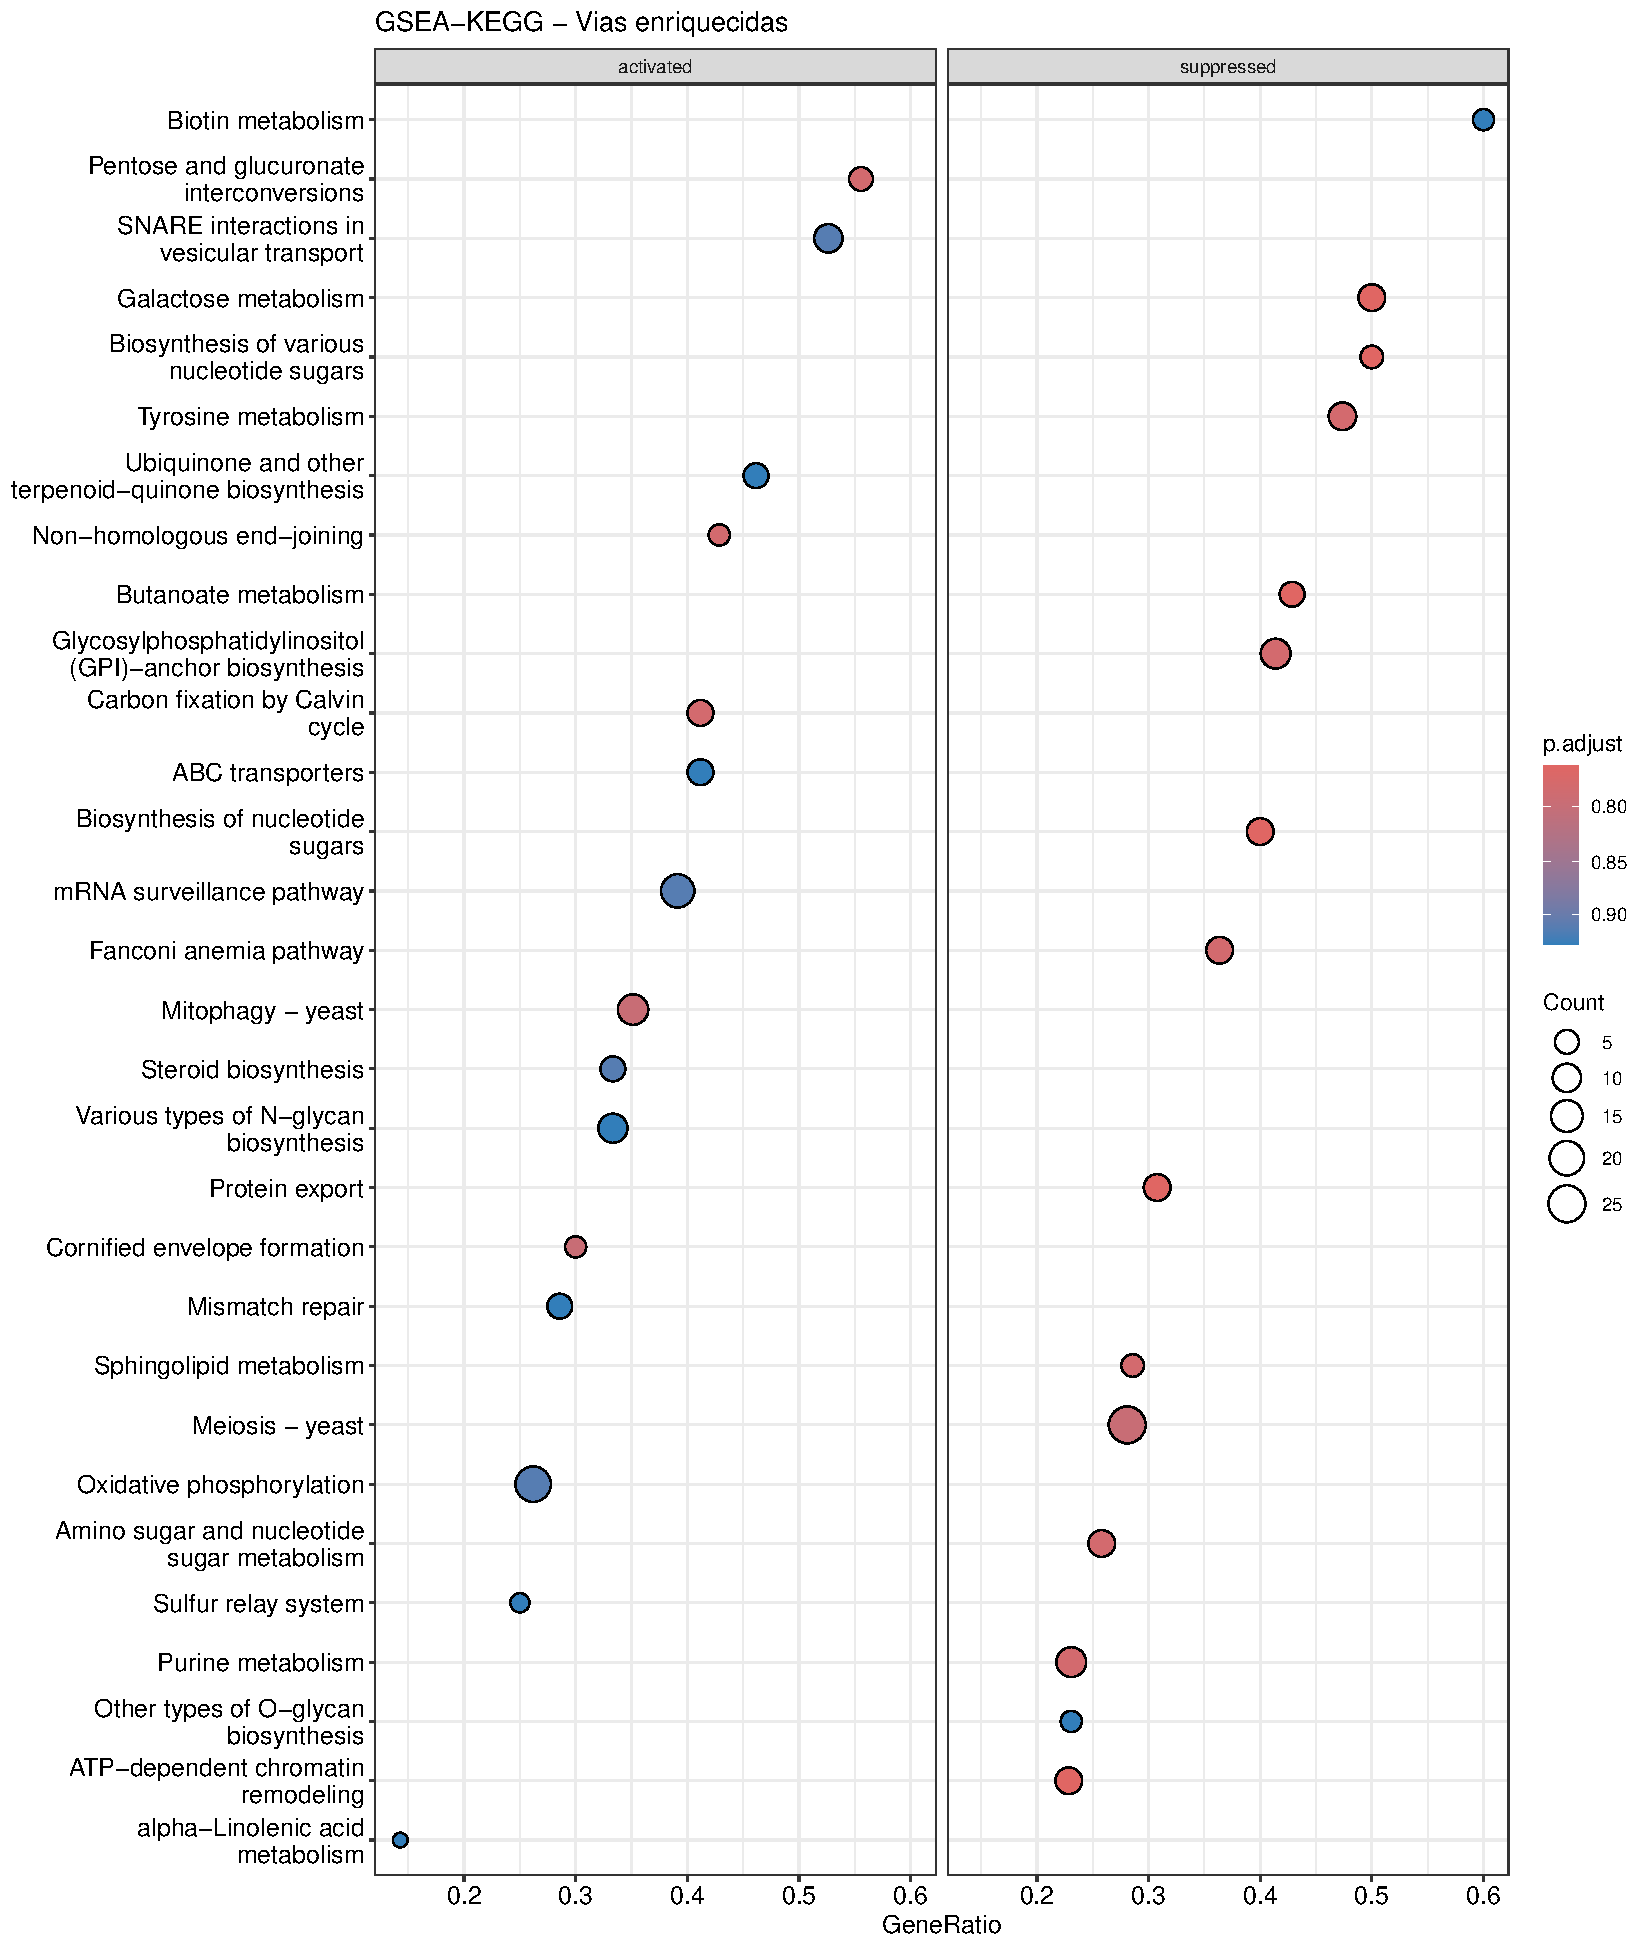
\includegraphics[keepaspectratio]{analysis/04_downstream_analyses_files/figure-pdf/unnamed-chunk-8-1.pdf}}

\subsection{Dotplot --- KEGG Todos os
DEGs}\label{dotplot-kegg-todos-os-degs}

\begin{Shaded}
\begin{Highlighting}[]
\ControlFlowTok{if}\NormalTok{ (}\SpecialCharTok{!}\FunctionTok{is.null}\NormalTok{(kegg\_all) }\SpecialCharTok{\&\&} \FunctionTok{nrow}\NormalTok{(}\FunctionTok{as.data.frame}\NormalTok{(kegg\_all)) }\SpecialCharTok{\textgreater{}} \DecValTok{0}\NormalTok{) \{}
  \FunctionTok{dotplot}\NormalTok{(kegg\_all,}
          \AttributeTok{showCategory =} \DecValTok{15}\NormalTok{,}
          \AttributeTok{title =} \StringTok{"KEGG — Todos os DEGs"}\NormalTok{,}
          \AttributeTok{color =} \StringTok{"p.adjust"}\NormalTok{) }\SpecialCharTok{+}
    \FunctionTok{theme}\NormalTok{(}\AttributeTok{axis.text.y =} \FunctionTok{element\_text}\NormalTok{(}\AttributeTok{size =} \DecValTok{10}\NormalTok{)) }\SpecialCharTok{+}
    \FunctionTok{scale\_color\_gradient}\NormalTok{(}\AttributeTok{low =} \StringTok{"grey20"}\NormalTok{, }\AttributeTok{high =} \StringTok{"grey70"}\NormalTok{, }\AttributeTok{name =} \StringTok{"p{-}valor}\SpecialCharTok{\textbackslash{}n}\StringTok{ajustado"}\NormalTok{)}
\NormalTok{\} }\ControlFlowTok{else}\NormalTok{ \{}
  \FunctionTok{cat}\NormalTok{(}\StringTok{"Nenhuma via KEGG enriquecida para todos os DEGs.}\SpecialCharTok{\textbackslash{}n}\StringTok{"}\NormalTok{)}
\NormalTok{\}}
\end{Highlighting}
\end{Shaded}

\pandocbounded{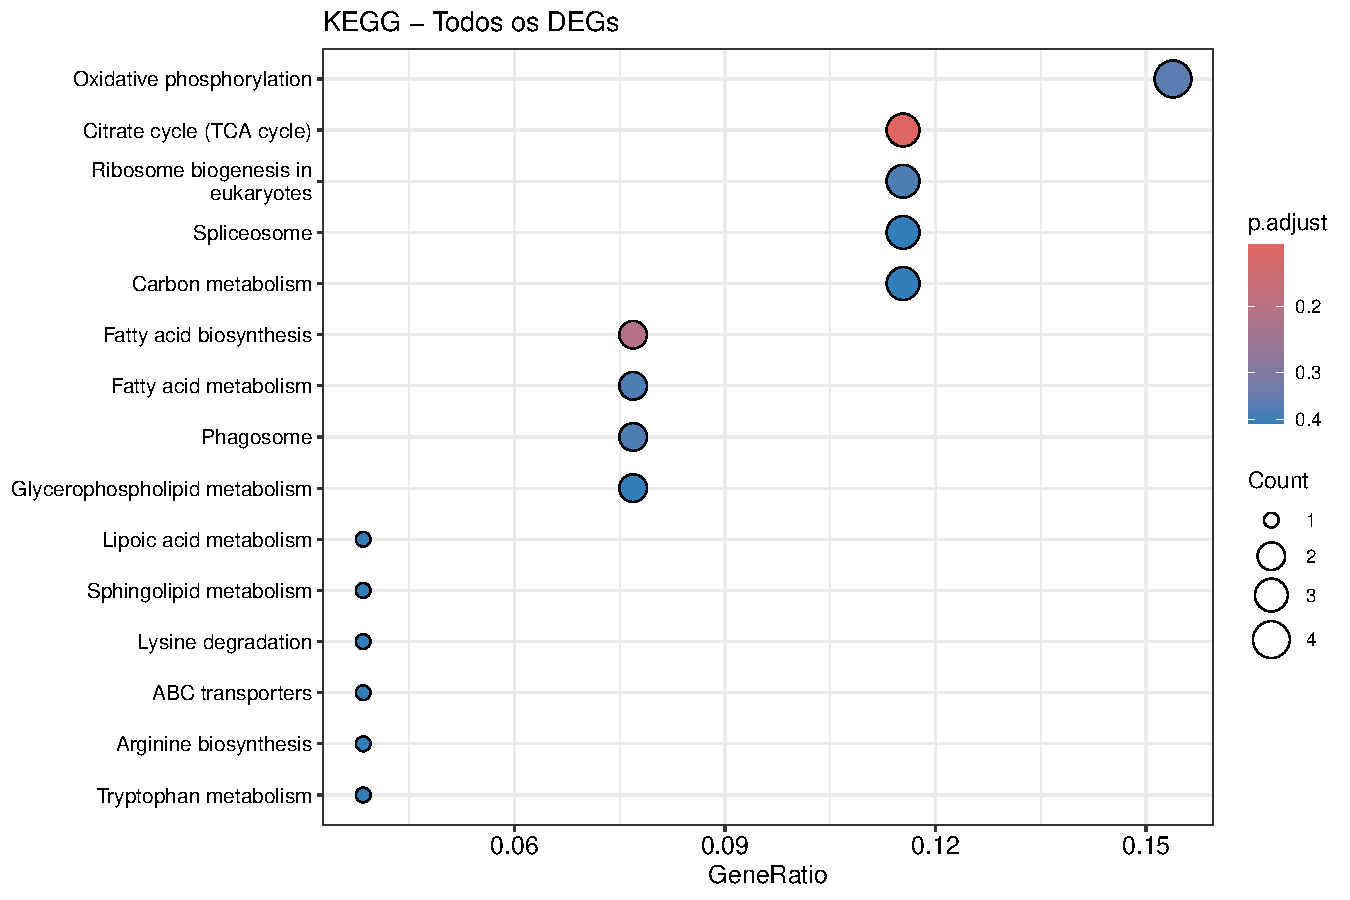
\includegraphics[keepaspectratio]{analysis/04_downstream_analyses_files/figure-pdf/unnamed-chunk-9-1.pdf}}

\subsection{Barplot Bidirecional --- KEGG UP
vs.~DOWN}\label{barplot-bidirecional-kegg-up-vs.-down}

Para comparar diretamente quais vias estão ativadas (UP) e reprimidas
(DOWN), podemos construir um \textbf{barplot bidirecional} onde as
barras vermelhas (UP) se estendem para a direita e as azuis (DOWN) para
a esquerda:

\begin{Shaded}
\begin{Highlighting}[]
\CommentTok{\# Extrair resultados de UP e DOWN}
\NormalTok{df\_kegg\_up }\OtherTok{\textless{}{-}} \ControlFlowTok{if}\NormalTok{ (}\SpecialCharTok{!}\FunctionTok{is.null}\NormalTok{(kegg\_up) }\SpecialCharTok{\&\&} \FunctionTok{nrow}\NormalTok{(}\FunctionTok{as.data.frame}\NormalTok{(kegg\_up)) }\SpecialCharTok{\textgreater{}} \DecValTok{0}\NormalTok{) \{}
  \FunctionTok{as.data.frame}\NormalTok{(kegg\_up) }\SpecialCharTok{\%\textgreater{}\%} \FunctionTok{mutate}\NormalTok{(}\AttributeTok{Direction =} \StringTok{"Upregulated"}\NormalTok{, }\AttributeTok{Count\_dir =}\NormalTok{ Count)}
\NormalTok{\} }\ControlFlowTok{else}\NormalTok{ \{ }\FunctionTok{data.frame}\NormalTok{() \}}

\NormalTok{df\_kegg\_down }\OtherTok{\textless{}{-}} \ControlFlowTok{if}\NormalTok{ (}\SpecialCharTok{!}\FunctionTok{is.null}\NormalTok{(kegg\_down) }\SpecialCharTok{\&\&} \FunctionTok{nrow}\NormalTok{(}\FunctionTok{as.data.frame}\NormalTok{(kegg\_down)) }\SpecialCharTok{\textgreater{}} \DecValTok{0}\NormalTok{) \{}
  \FunctionTok{as.data.frame}\NormalTok{(kegg\_down) }\SpecialCharTok{\%\textgreater{}\%} \FunctionTok{mutate}\NormalTok{(}\AttributeTok{Direction =} \StringTok{"Downregulated"}\NormalTok{, }\AttributeTok{Count\_dir =} \SpecialCharTok{{-}}\NormalTok{Count)}
\NormalTok{\} }\ControlFlowTok{else}\NormalTok{ \{ }\FunctionTok{data.frame}\NormalTok{() \}}

\ControlFlowTok{if}\NormalTok{ (}\FunctionTok{nrow}\NormalTok{(df\_kegg\_up) }\SpecialCharTok{\textgreater{}} \DecValTok{0} \SpecialCharTok{||} \FunctionTok{nrow}\NormalTok{(df\_kegg\_down) }\SpecialCharTok{\textgreater{}} \DecValTok{0}\NormalTok{) \{}
\NormalTok{  df\_kegg\_bidir }\OtherTok{\textless{}{-}} \FunctionTok{bind\_rows}\NormalTok{(}
\NormalTok{    df\_kegg\_up }\SpecialCharTok{\%\textgreater{}\%} \FunctionTok{head}\NormalTok{(}\DecValTok{10}\NormalTok{),}
\NormalTok{    df\_kegg\_down }\SpecialCharTok{\%\textgreater{}\%} \FunctionTok{head}\NormalTok{(}\DecValTok{10}\NormalTok{)}
\NormalTok{  )}

  \FunctionTok{ggplot}\NormalTok{(df\_kegg\_bidir, }\FunctionTok{aes}\NormalTok{(}\AttributeTok{x =}\NormalTok{ Count\_dir, }\AttributeTok{y =} \FunctionTok{reorder}\NormalTok{(Description, Count\_dir), }\AttributeTok{fill =}\NormalTok{ Direction)) }\SpecialCharTok{+}
    \FunctionTok{geom\_col}\NormalTok{(}\AttributeTok{width =} \FloatTok{0.7}\NormalTok{) }\SpecialCharTok{+}
    \FunctionTok{scale\_fill\_manual}\NormalTok{(}\AttributeTok{values =} \FunctionTok{c}\NormalTok{(}\StringTok{"Upregulated"} \OtherTok{=} \StringTok{"\#E31A1C"}\NormalTok{, }\StringTok{"Downregulated"} \OtherTok{=} \StringTok{"\#1F78B4"}\NormalTok{)) }\SpecialCharTok{+}
    \FunctionTok{geom\_vline}\NormalTok{(}\AttributeTok{xintercept =} \DecValTok{0}\NormalTok{, }\AttributeTok{linewidth =} \FloatTok{0.5}\NormalTok{) }\SpecialCharTok{+}
    \FunctionTok{labs}\NormalTok{(}\AttributeTok{title =} \StringTok{"KEGG — UP vs. DOWN"}\NormalTok{,}
         \AttributeTok{x =} \StringTok{"Número de Genes"}\NormalTok{, }\AttributeTok{y =} \ConstantTok{NULL}\NormalTok{, }\AttributeTok{fill =} \StringTok{"Regulação"}\NormalTok{) }\SpecialCharTok{+}
    \FunctionTok{theme\_minimal}\NormalTok{(}\AttributeTok{base\_size =} \DecValTok{13}\NormalTok{) }\SpecialCharTok{+}
    \FunctionTok{theme}\NormalTok{(}\AttributeTok{plot.title =} \FunctionTok{element\_text}\NormalTok{(}\AttributeTok{hjust =} \FloatTok{0.5}\NormalTok{, }\AttributeTok{face =} \StringTok{"bold"}\NormalTok{),}
          \AttributeTok{axis.text.y =} \FunctionTok{element\_text}\NormalTok{(}\AttributeTok{size =} \DecValTok{9}\NormalTok{),}
          \AttributeTok{legend.position =} \StringTok{"bottom"}\NormalTok{)}
\NormalTok{\} }\ControlFlowTok{else}\NormalTok{ \{}
  \FunctionTok{cat}\NormalTok{(}\StringTok{"Nenhuma via KEGG enriquecida para gerar o barplot bidirecional.}\SpecialCharTok{\textbackslash{}n}\StringTok{"}\NormalTok{)}
\NormalTok{\}}
\end{Highlighting}
\end{Shaded}

\pandocbounded{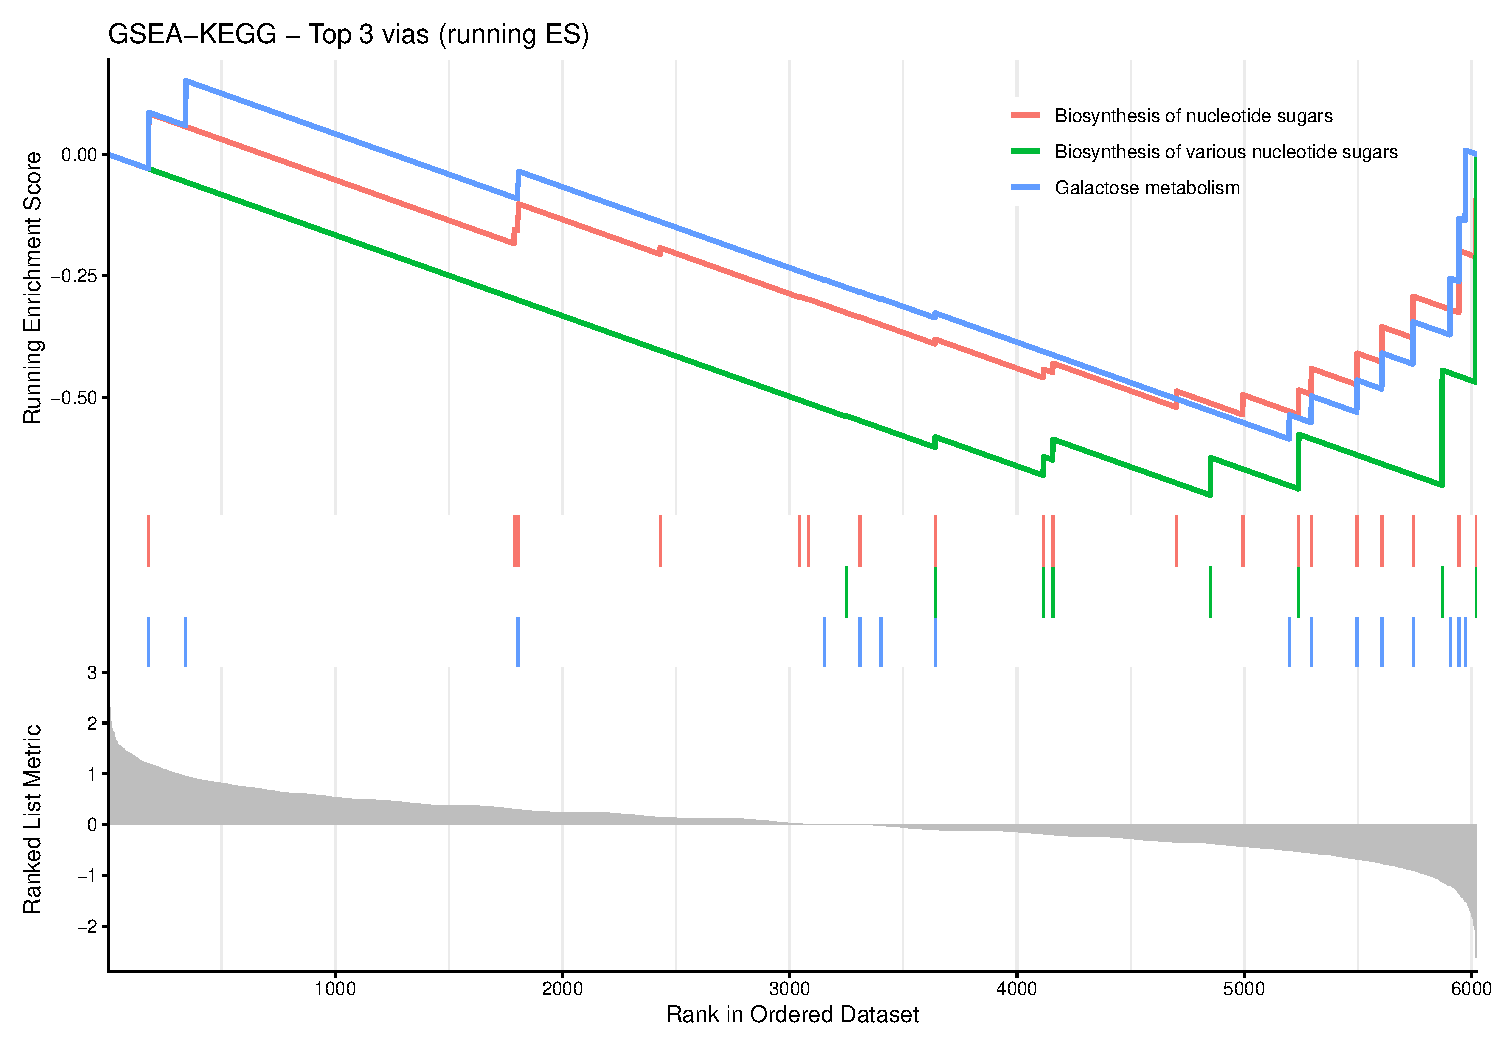
\includegraphics[keepaspectratio]{analysis/04_downstream_analyses_files/figure-pdf/unnamed-chunk-10-1.pdf}}

\subsection{Barplot --- KEGG Todos os
DEGs}\label{barplot-kegg-todos-os-degs}

\begin{Shaded}
\begin{Highlighting}[]
\ControlFlowTok{if}\NormalTok{ (}\SpecialCharTok{!}\FunctionTok{is.null}\NormalTok{(kegg\_all) }\SpecialCharTok{\&\&} \FunctionTok{nrow}\NormalTok{(}\FunctionTok{as.data.frame}\NormalTok{(kegg\_all)) }\SpecialCharTok{\textgreater{}} \DecValTok{0}\NormalTok{) \{}
  \FunctionTok{barplot}\NormalTok{(kegg\_all,}
          \AttributeTok{showCategory =} \DecValTok{15}\NormalTok{,}
          \AttributeTok{title =} \StringTok{"KEGG — Todos os DEGs"}\NormalTok{,}
          \AttributeTok{color =} \StringTok{"p.adjust"}\NormalTok{) }\SpecialCharTok{+}
    \FunctionTok{theme}\NormalTok{(}\AttributeTok{axis.text.y =} \FunctionTok{element\_text}\NormalTok{(}\AttributeTok{size =} \DecValTok{10}\NormalTok{)) }\SpecialCharTok{+}
    \FunctionTok{scale\_fill\_gradient}\NormalTok{(}\AttributeTok{low =} \StringTok{"grey20"}\NormalTok{, }\AttributeTok{high =} \StringTok{"grey70"}\NormalTok{, }\AttributeTok{name =} \StringTok{"p{-}valor}\SpecialCharTok{\textbackslash{}n}\StringTok{ajustado"}\NormalTok{)}
\NormalTok{\} }\ControlFlowTok{else}\NormalTok{ \{}
  \FunctionTok{cat}\NormalTok{(}\StringTok{"Nenhuma via KEGG enriquecida para todos os DEGs.}\SpecialCharTok{\textbackslash{}n}\StringTok{"}\NormalTok{)}
\NormalTok{\}}
\end{Highlighting}
\end{Shaded}

\pandocbounded{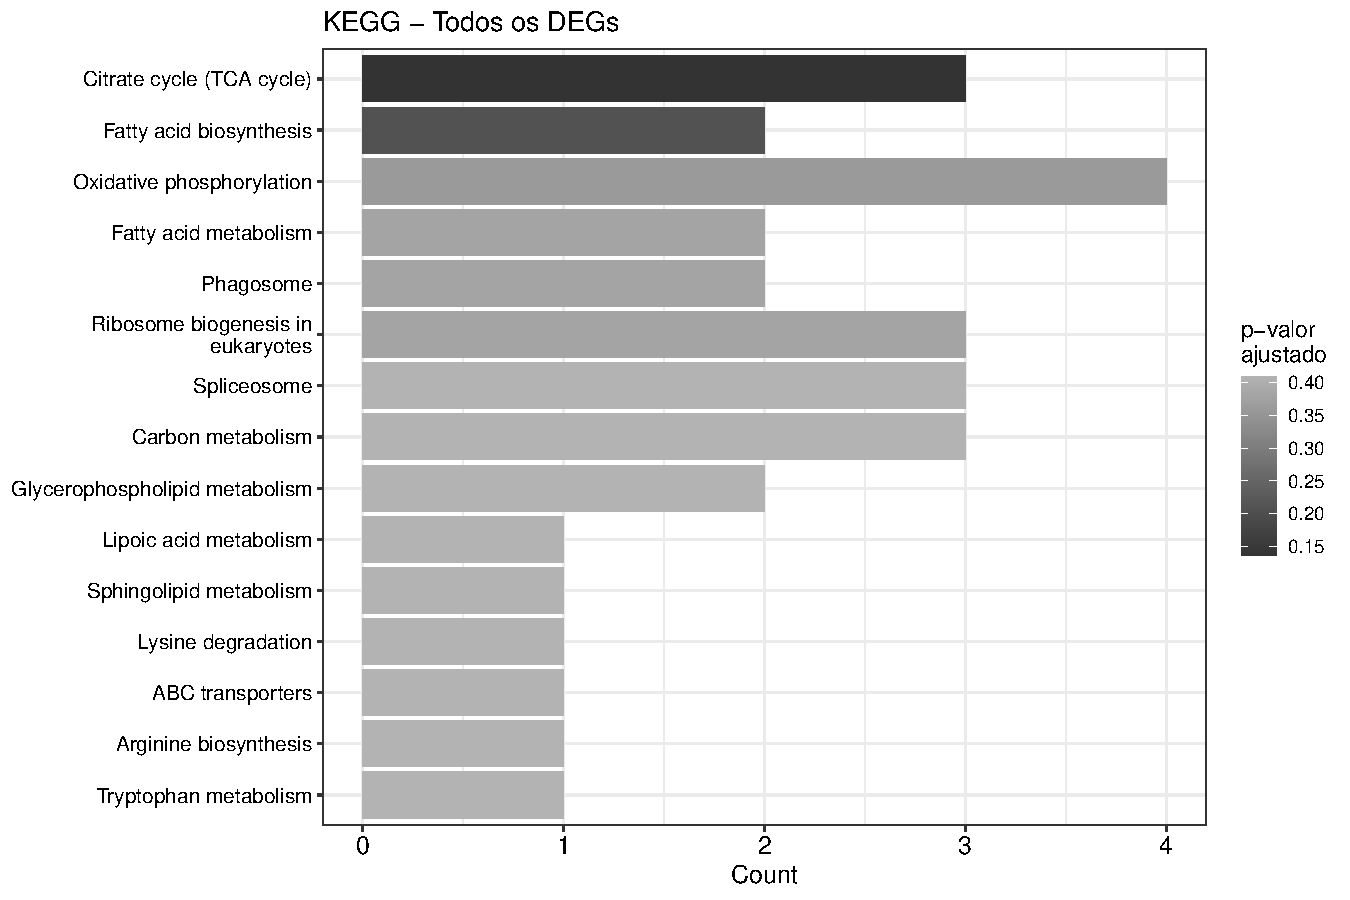
\includegraphics[keepaspectratio]{analysis/04_downstream_analyses_files/figure-pdf/unnamed-chunk-11-1.pdf}}

\subsection{Como interpretar os
gráficos:}\label{como-interpretar-os-gruxe1ficos}

\begin{itemize}
\tightlist
\item
  \textbf{Dotplot}: cada ponto representa uma via enriquecida. O
  \textbf{tamanho} indica quantos DEGs pertencem àquela via (Count); a
  \textbf{cor} indica o p-valor ajustado.
\item
  \textbf{Barplot bidirecional}: permite comparar diretamente as vias UP
  (vermelho, à direita) e DOWN (azul, à esquerda) em um único gráfico.
\item
  \textbf{Barplot (ALL)}: mostra as vias enriquecidas considerando todos
  os DEGs juntos, com a cor indicando o p-valor ajustado.
\end{itemize}

\begin{center}\rule{0.5\linewidth}{0.5pt}\end{center}

\section{6. Obtendo Anotações GO do Candida Genome Database
(CGD)}\label{obtendo-anotauxe7uxf5es-go-do-candida-genome-database-cgd}

O \textbf{Candida Genome Database (CGD)} disponibiliza um arquivo GAF
(\emph{Gene Association File}) com anotações de Gene Ontology curadas
manualmente e computacionalmente, específicas para \emph{C. albicans}
SC5314. Esse arquivo contém mais de 33 mil anotações ---
significativamente mais completo do que o disponível via Ensembl Fungi.

\begin{tcolorbox}[enhanced jigsaw, arc=.35mm, bottomrule=.15mm, bottomtitle=1mm, breakable, colback=white, colbacktitle=quarto-callout-note-color!10!white, colframe=quarto-callout-note-color-frame, coltitle=black, left=2mm, leftrule=.75mm, opacityback=0, opacitybacktitle=0.6, rightrule=.15mm, title=\textcolor{quarto-callout-note-color}{\faInfo}\hspace{0.5em}{Ponto Importante}, titlerule=0mm, toprule=.15mm, toptitle=1mm]

O arquivo GAF pode ser baixado diretamente de:
\href{http://www.candidagenome.org/download/go/}{candidagenome.org/download/go/}.
Nós já o baixamos e descompactamos em \texttt{data/cgd/}.

\end{tcolorbox}

\subsection{Parsear o arquivo GAF}\label{parsear-o-arquivo-gaf}

\begin{Shaded}
\begin{Highlighting}[]
\CommentTok{\# Ler o arquivo GAF (pulando linhas de comentário)}
\NormalTok{gaf\_raw }\OtherTok{\textless{}{-}} \FunctionTok{read.delim}\NormalTok{(}
\NormalTok{  here}\SpecialCharTok{::}\FunctionTok{here}\NormalTok{(}\StringTok{"data/cgd/cgd\_C\_albicans\_SC5314.gaf"}\NormalTok{),}
  \AttributeTok{header =} \ConstantTok{FALSE}\NormalTok{,}
  \AttributeTok{comment.char =} \StringTok{"!"}\NormalTok{,}
  \AttributeTok{quote =} \StringTok{""}\NormalTok{,}
  \AttributeTok{stringsAsFactors =} \ConstantTok{FALSE}
\NormalTok{)}

\CommentTok{\# Nomear as colunas relevantes do GAF 2.2}
\FunctionTok{colnames}\NormalTok{(gaf\_raw)[}\FunctionTok{c}\NormalTok{(}\DecValTok{1}\NormalTok{, }\DecValTok{2}\NormalTok{, }\DecValTok{3}\NormalTok{, }\DecValTok{4}\NormalTok{, }\DecValTok{5}\NormalTok{, }\DecValTok{7}\NormalTok{, }\DecValTok{9}\NormalTok{, }\DecValTok{11}\NormalTok{)] }\OtherTok{\textless{}{-}} \FunctionTok{c}\NormalTok{(}
  \StringTok{"DB"}\NormalTok{, }\StringTok{"DB\_Object\_ID"}\NormalTok{, }\StringTok{"Gene\_Symbol"}\NormalTok{, }\StringTok{"Qualifier"}\NormalTok{, }\StringTok{"GO\_ID"}\NormalTok{,}
  \StringTok{"Evidence\_Code"}\NormalTok{, }\StringTok{"Aspect"}\NormalTok{, }\StringTok{"Synonyms"}
\NormalTok{)}

\FunctionTok{cat}\NormalTok{(}\StringTok{"Total de anotações no GAF:"}\NormalTok{, }\FunctionTok{nrow}\NormalTok{(gaf\_raw), }\StringTok{"}\SpecialCharTok{\textbackslash{}n}\StringTok{"}\NormalTok{)}
\end{Highlighting}
\end{Shaded}

\begin{verbatim}
Total de anotações no GAF: 33286 
\end{verbatim}

\subsection{Extrair IDs Ensembl dos
Sinônimos}\label{extrair-ids-ensembl-dos-sinuxf4nimos}

\begin{Shaded}
\begin{Highlighting}[]
\CommentTok{\# Função para extrair o ID Ensembl (\_A) dos sinônimos}
\NormalTok{extract\_ensembl\_id }\OtherTok{\textless{}{-}} \ControlFlowTok{function}\NormalTok{(synonyms) \{}
\NormalTok{  syns }\OtherTok{\textless{}{-}} \FunctionTok{unlist}\NormalTok{(}\FunctionTok{strsplit}\NormalTok{(synonyms, }\StringTok{"}\SpecialCharTok{\textbackslash{}\textbackslash{}}\StringTok{|"}\NormalTok{))}
\NormalTok{  match }\OtherTok{\textless{}{-}} \FunctionTok{grep}\NormalTok{(}\StringTok{"\^{}C[0{-}9R]+\_}\SpecialCharTok{\textbackslash{}\textbackslash{}}\StringTok{d\{5\}[WC]\_A$"}\NormalTok{, syns, }\AttributeTok{value =} \ConstantTok{TRUE}\NormalTok{)}
  \ControlFlowTok{if}\NormalTok{ (}\FunctionTok{length}\NormalTok{(match) }\SpecialCharTok{\textgreater{}} \DecValTok{0}\NormalTok{) }\FunctionTok{return}\NormalTok{(match[}\DecValTok{1}\NormalTok{])}
  \FunctionTok{return}\NormalTok{(}\ConstantTok{NA\_character\_}\NormalTok{)}
\NormalTok{\}}

\CommentTok{\# Aplicar a extração}
\NormalTok{gaf\_raw}\SpecialCharTok{$}\NormalTok{ensembl\_id }\OtherTok{\textless{}{-}} \FunctionTok{sapply}\NormalTok{(gaf\_raw}\SpecialCharTok{$}\NormalTok{Synonyms, extract\_ensembl\_id)}

\CommentTok{\# Verificar taxa de mapeamento}
\NormalTok{mapped }\OtherTok{\textless{}{-}} \FunctionTok{sum}\NormalTok{(}\SpecialCharTok{!}\FunctionTok{is.na}\NormalTok{(gaf\_raw}\SpecialCharTok{$}\NormalTok{ensembl\_id))}
\FunctionTok{cat}\NormalTok{(}\StringTok{"Anotações com ID Ensembl mapeado:"}\NormalTok{, mapped, }\StringTok{"de"}\NormalTok{, }\FunctionTok{nrow}\NormalTok{(gaf\_raw), }\StringTok{"}\SpecialCharTok{\textbackslash{}n}\StringTok{"}\NormalTok{)}
\end{Highlighting}
\end{Shaded}

\begin{verbatim}
Anotações com ID Ensembl mapeado: 33028 de 33286 
\end{verbatim}

\subsection{Construir TERM2GENE e
TERM2NAME}\label{construir-term2gene-e-term2name}

\begin{Shaded}
\begin{Highlighting}[]
\CommentTok{\# Filtrar anotações válidas}
\NormalTok{gaf\_mapped }\OtherTok{\textless{}{-}}\NormalTok{ gaf\_raw }\SpecialCharTok{\%\textgreater{}\%}
  \FunctionTok{filter}\NormalTok{(}\SpecialCharTok{!}\FunctionTok{is.na}\NormalTok{(ensembl\_id)) }\SpecialCharTok{\%\textgreater{}\%}
\NormalTok{  dplyr}\SpecialCharTok{::}\FunctionTok{select}\NormalTok{(ensembl\_id, GO\_ID, Gene\_Symbol, Aspect)}

\CommentTok{\# TERM2GENE: GO\_ID → ensembl\_id}
\NormalTok{term2gene\_cgd }\OtherTok{\textless{}{-}}\NormalTok{ gaf\_mapped }\SpecialCharTok{\%\textgreater{}\%}
\NormalTok{  dplyr}\SpecialCharTok{::}\FunctionTok{select}\NormalTok{(GO\_ID, ensembl\_id) }\SpecialCharTok{\%\textgreater{}\%}
  \FunctionTok{distinct}\NormalTok{()}

\CommentTok{\# Obter nomes dos termos GO via GO.db}
\NormalTok{go\_terms }\OtherTok{\textless{}{-}}\NormalTok{ AnnotationDbi}\SpecialCharTok{::}\FunctionTok{select}\NormalTok{(GO.db, }
                                   \AttributeTok{keys =} \FunctionTok{unique}\NormalTok{(term2gene\_cgd}\SpecialCharTok{$}\NormalTok{GO\_ID), }
                                   \AttributeTok{columns =} \FunctionTok{c}\NormalTok{(}\StringTok{"GOID"}\NormalTok{, }\StringTok{"TERM"}\NormalTok{, }\StringTok{"ONTOLOGY"}\NormalTok{), }
                                   \AttributeTok{keytype =} \StringTok{"GOID"}\NormalTok{)}
\NormalTok{go\_terms }\OtherTok{\textless{}{-}}\NormalTok{ go\_terms[}\SpecialCharTok{!}\FunctionTok{is.na}\NormalTok{(go\_terms}\SpecialCharTok{$}\NormalTok{TERM), ]}

\NormalTok{term2name\_cgd }\OtherTok{\textless{}{-}} \FunctionTok{data.frame}\NormalTok{(}
  \AttributeTok{GO\_ID =}\NormalTok{ go\_terms}\SpecialCharTok{$}\NormalTok{GOID,}
  \AttributeTok{Name =}\NormalTok{ go\_terms}\SpecialCharTok{$}\NormalTok{TERM}
\NormalTok{)}

\FunctionTok{cat}\NormalTok{(}\StringTok{"Total de mapeamentos gene{-}GO:"}\NormalTok{, }\FunctionTok{nrow}\NormalTok{(term2gene\_cgd), }\StringTok{"}\SpecialCharTok{\textbackslash{}n}\StringTok{"}\NormalTok{)}
\end{Highlighting}
\end{Shaded}

\begin{verbatim}
Total de mapeamentos gene-GO: 29905 
\end{verbatim}

\begin{Shaded}
\begin{Highlighting}[]
\FunctionTok{cat}\NormalTok{(}\StringTok{"Termos GO únicos:"}\NormalTok{, }\FunctionTok{length}\NormalTok{(}\FunctionTok{unique}\NormalTok{(term2gene\_cgd}\SpecialCharTok{$}\NormalTok{GO\_ID)), }\StringTok{"}\SpecialCharTok{\textbackslash{}n}\StringTok{"}\NormalTok{)}
\end{Highlighting}
\end{Shaded}

\begin{verbatim}
Termos GO únicos: 3277 
\end{verbatim}

\begin{Shaded}
\begin{Highlighting}[]
\FunctionTok{cat}\NormalTok{(}\StringTok{"Genes únicos com GO:"}\NormalTok{, }\FunctionTok{length}\NormalTok{(}\FunctionTok{unique}\NormalTok{(term2gene\_cgd}\SpecialCharTok{$}\NormalTok{ensembl\_id)), }\StringTok{"}\SpecialCharTok{\textbackslash{}n}\StringTok{"}\NormalTok{)}
\end{Highlighting}
\end{Shaded}

\begin{verbatim}
Genes únicos com GO: 6261 
\end{verbatim}

\begin{Shaded}
\begin{Highlighting}[]
\CommentTok{\# Separar por ontologia}
\NormalTok{bp\_terms }\OtherTok{\textless{}{-}}\NormalTok{ go\_terms }\SpecialCharTok{\%\textgreater{}\%} \FunctionTok{filter}\NormalTok{(ONTOLOGY }\SpecialCharTok{==} \StringTok{"BP"}\NormalTok{)}

\NormalTok{term2gene\_cgd\_bp }\OtherTok{\textless{}{-}}\NormalTok{ term2gene\_cgd }\SpecialCharTok{\%\textgreater{}\%} \FunctionTok{filter}\NormalTok{(GO\_ID }\SpecialCharTok{\%in\%}\NormalTok{ bp\_terms}\SpecialCharTok{$}\NormalTok{GOID)}
\NormalTok{term2name\_cgd\_bp }\OtherTok{\textless{}{-}}\NormalTok{ term2name\_cgd }\SpecialCharTok{\%\textgreater{}\%} \FunctionTok{filter}\NormalTok{(GO\_ID }\SpecialCharTok{\%in\%}\NormalTok{ bp\_terms}\SpecialCharTok{$}\NormalTok{GOID)}

\FunctionTok{cat}\NormalTok{(}\StringTok{"Termos BP:"}\NormalTok{, }\FunctionTok{length}\NormalTok{(}\FunctionTok{unique}\NormalTok{(term2gene\_cgd\_bp}\SpecialCharTok{$}\NormalTok{GO\_ID)), }\StringTok{"}\SpecialCharTok{\textbackslash{}n}\StringTok{"}\NormalTok{)}
\end{Highlighting}
\end{Shaded}

\begin{verbatim}
Termos BP: 1661 
\end{verbatim}

\begin{center}\rule{0.5\linewidth}{0.5pt}\end{center}

\section{7. Enriquecimento GO --- ORA
(CGD)}\label{enriquecimento-go-ora-cgd}

Vamos rodar a ORA com Gene Ontology (Biological Process) separadamente
para cada conjunto:

\begin{Shaded}
\begin{Highlighting}[]
\CommentTok{\# GO ORA — Upregulados}
\NormalTok{go\_up }\OtherTok{\textless{}{-}} \FunctionTok{enricher}\NormalTok{(}
  \AttributeTok{gene =}\NormalTok{ genes\_up,}
  \AttributeTok{TERM2GENE =}\NormalTok{ term2gene\_cgd\_bp,}
  \AttributeTok{TERM2NAME =}\NormalTok{ term2name\_cgd\_bp,}
  \AttributeTok{pvalueCutoff =} \FloatTok{0.5}\NormalTok{, }\AttributeTok{qvalueCutoff =} \FloatTok{0.5}\NormalTok{, }\AttributeTok{pAdjustMethod =} \StringTok{"BH"}
\NormalTok{)}

\CommentTok{\# GO ORA — Downregulados}
\NormalTok{go\_down }\OtherTok{\textless{}{-}} \FunctionTok{enricher}\NormalTok{(}
  \AttributeTok{gene =}\NormalTok{ genes\_down,}
  \AttributeTok{TERM2GENE =}\NormalTok{ term2gene\_cgd\_bp,}
  \AttributeTok{TERM2NAME =}\NormalTok{ term2name\_cgd\_bp,}
  \AttributeTok{pvalueCutoff =} \FloatTok{0.5}\NormalTok{, }\AttributeTok{qvalueCutoff =} \FloatTok{0.5}\NormalTok{, }\AttributeTok{pAdjustMethod =} \StringTok{"BH"}
\NormalTok{)}

\CommentTok{\# GO ORA — Todos os DEGs}
\NormalTok{go\_all }\OtherTok{\textless{}{-}} \FunctionTok{enricher}\NormalTok{(}
  \AttributeTok{gene =}\NormalTok{ genes\_all,}
  \AttributeTok{TERM2GENE =}\NormalTok{ term2gene\_cgd\_bp,}
  \AttributeTok{TERM2NAME =}\NormalTok{ term2name\_cgd\_bp,}
  \AttributeTok{pvalueCutoff =} \FloatTok{0.5}\NormalTok{, }\AttributeTok{qvalueCutoff =} \FloatTok{0.5}\NormalTok{, }\AttributeTok{pAdjustMethod =} \StringTok{"BH"}
\NormalTok{)}
\end{Highlighting}
\end{Shaded}

\subsection{Dotplot --- GO BP
Upregulados}\label{dotplot-go-bp-upregulados}

\begin{Shaded}
\begin{Highlighting}[]
\ControlFlowTok{if}\NormalTok{ (}\SpecialCharTok{!}\FunctionTok{is.null}\NormalTok{(go\_up) }\SpecialCharTok{\&\&} \FunctionTok{nrow}\NormalTok{(}\FunctionTok{as.data.frame}\NormalTok{(go\_up)) }\SpecialCharTok{\textgreater{}} \DecValTok{0}\NormalTok{) \{}
  \FunctionTok{dotplot}\NormalTok{(go\_up,}
          \AttributeTok{showCategory =} \DecValTok{15}\NormalTok{,}
          \AttributeTok{title =} \StringTok{"GO Biological Process — Genes Upregulados (CGD)"}\NormalTok{,}
          \AttributeTok{color =} \StringTok{"p.adjust"}\NormalTok{) }\SpecialCharTok{+}
    \FunctionTok{theme}\NormalTok{(}\AttributeTok{axis.text.y =} \FunctionTok{element\_text}\NormalTok{(}\AttributeTok{size =} \DecValTok{9}\NormalTok{)) }\SpecialCharTok{+}
    \FunctionTok{scale\_color\_gradient}\NormalTok{(}\AttributeTok{low =} \StringTok{"\#E31A1C"}\NormalTok{, }\AttributeTok{high =} \StringTok{"\#FCBBA1"}\NormalTok{, }\AttributeTok{name =} \StringTok{"p{-}valor}\SpecialCharTok{\textbackslash{}n}\StringTok{ajustado"}\NormalTok{)}
\NormalTok{\} }\ControlFlowTok{else}\NormalTok{ \{}
  \FunctionTok{cat}\NormalTok{(}\StringTok{"Nenhum processo biológico enriquecido para genes upregulados.}\SpecialCharTok{\textbackslash{}n}\StringTok{"}\NormalTok{)}
\NormalTok{\}}
\end{Highlighting}
\end{Shaded}

\pandocbounded{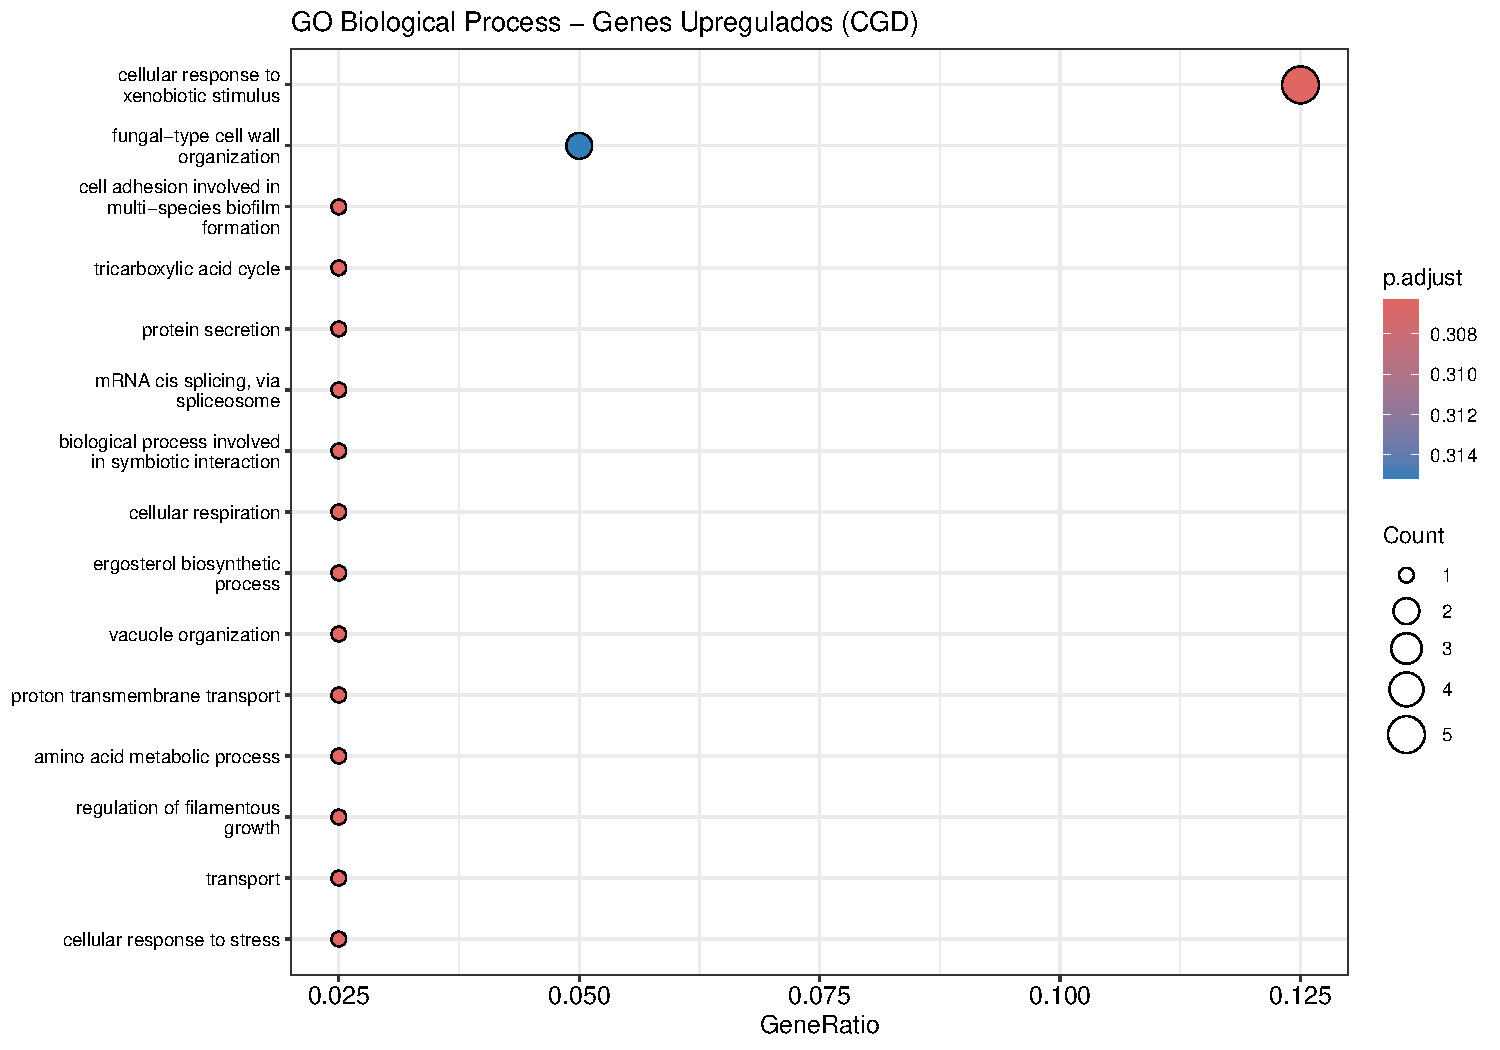
\includegraphics[keepaspectratio]{analysis/04_downstream_analyses_files/figure-pdf/unnamed-chunk-17-1.pdf}}

\subsection{Dotplot --- GO BP
Downregulados}\label{dotplot-go-bp-downregulados}

\begin{Shaded}
\begin{Highlighting}[]
\ControlFlowTok{if}\NormalTok{ (}\SpecialCharTok{!}\FunctionTok{is.null}\NormalTok{(go\_down) }\SpecialCharTok{\&\&} \FunctionTok{nrow}\NormalTok{(}\FunctionTok{as.data.frame}\NormalTok{(go\_down)) }\SpecialCharTok{\textgreater{}} \DecValTok{0}\NormalTok{) \{}
  \FunctionTok{dotplot}\NormalTok{(go\_down,}
          \AttributeTok{showCategory =} \DecValTok{15}\NormalTok{,}
          \AttributeTok{title =} \StringTok{"GO Biological Process — Genes Downregulados (CGD)"}\NormalTok{,}
          \AttributeTok{color =} \StringTok{"p.adjust"}\NormalTok{) }\SpecialCharTok{+}
    \FunctionTok{theme}\NormalTok{(}\AttributeTok{axis.text.y =} \FunctionTok{element\_text}\NormalTok{(}\AttributeTok{size =} \DecValTok{9}\NormalTok{)) }\SpecialCharTok{+}
    \FunctionTok{scale\_color\_gradient}\NormalTok{(}\AttributeTok{low =} \StringTok{"\#1F78B4"}\NormalTok{, }\AttributeTok{high =} \StringTok{"\#C6DBEF"}\NormalTok{, }\AttributeTok{name =} \StringTok{"p{-}valor}\SpecialCharTok{\textbackslash{}n}\StringTok{ajustado"}\NormalTok{)}
\NormalTok{\} }\ControlFlowTok{else}\NormalTok{ \{}
  \FunctionTok{cat}\NormalTok{(}\StringTok{"Nenhum processo biológico enriquecido para genes downregulados.}\SpecialCharTok{\textbackslash{}n}\StringTok{"}\NormalTok{)}
\NormalTok{\}}
\end{Highlighting}
\end{Shaded}

\pandocbounded{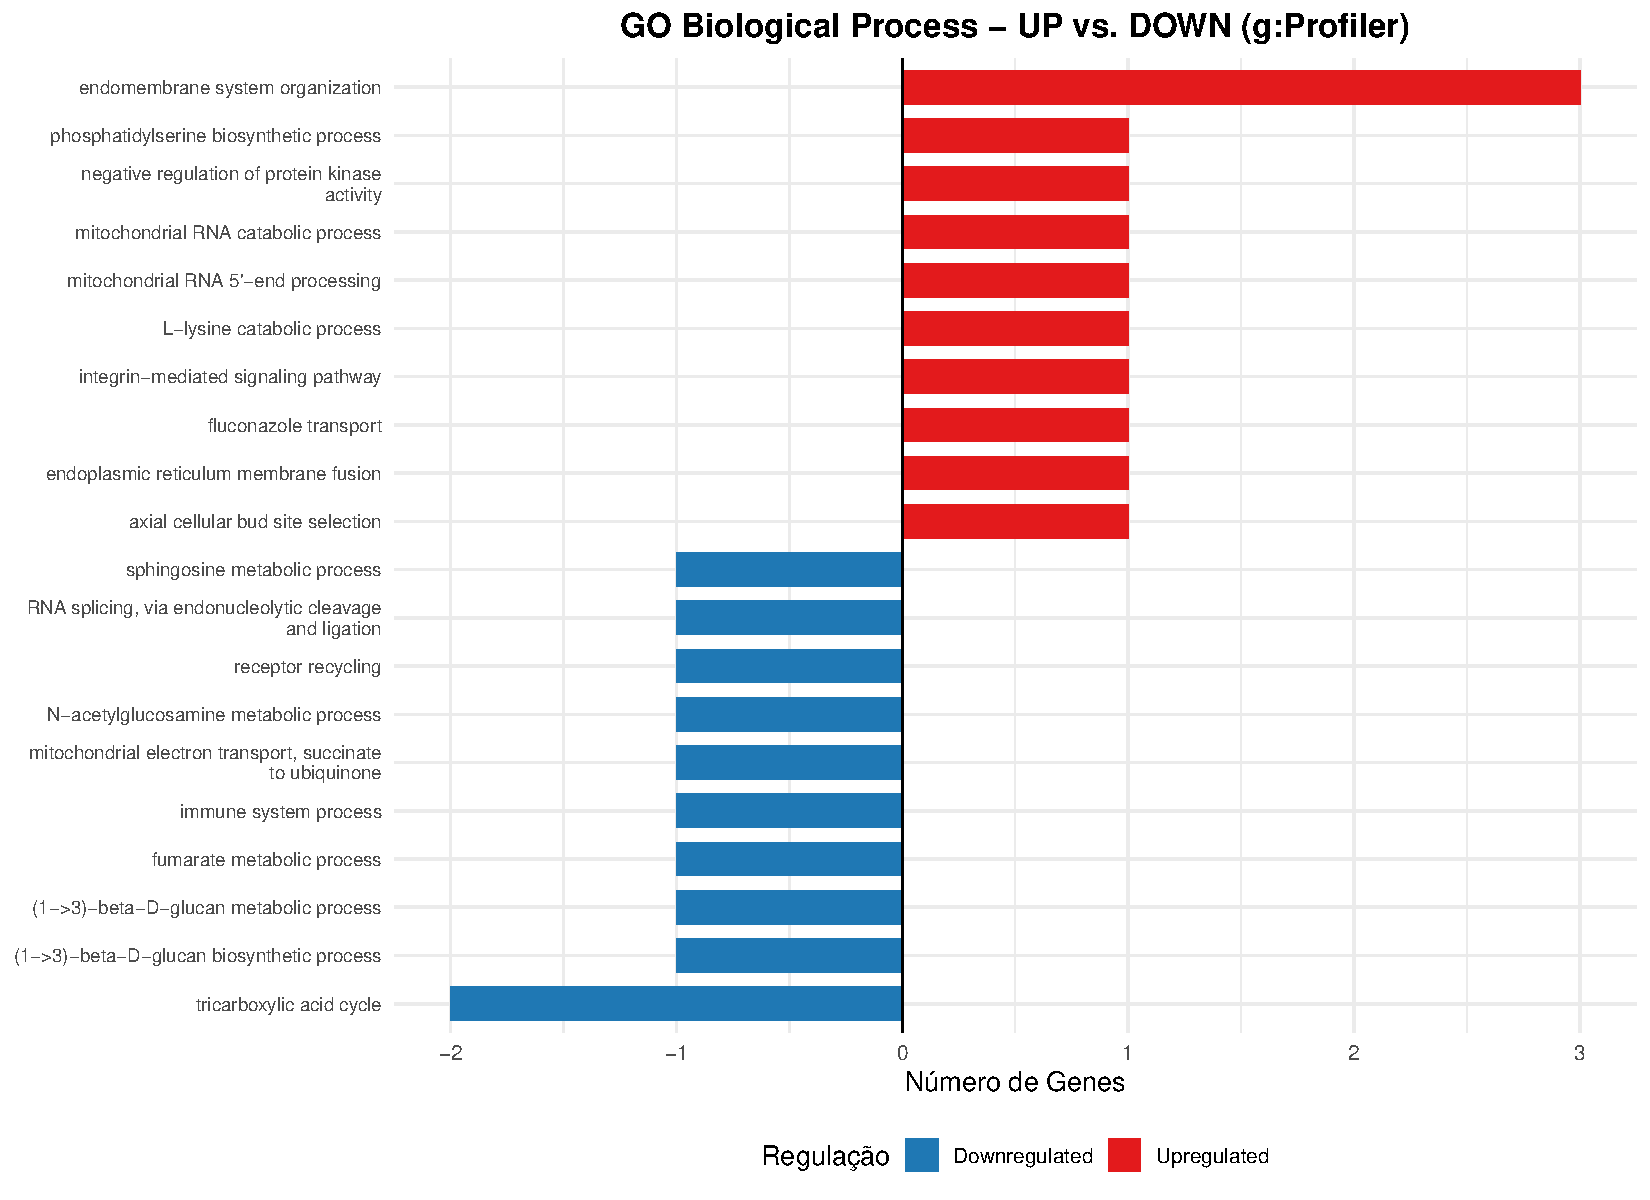
\includegraphics[keepaspectratio]{analysis/04_downstream_analyses_files/figure-pdf/unnamed-chunk-18-1.pdf}}

\subsection{Dotplot --- GO BP Todos os
DEGs}\label{dotplot-go-bp-todos-os-degs}

\begin{Shaded}
\begin{Highlighting}[]
\ControlFlowTok{if}\NormalTok{ (}\SpecialCharTok{!}\FunctionTok{is.null}\NormalTok{(go\_all) }\SpecialCharTok{\&\&} \FunctionTok{nrow}\NormalTok{(}\FunctionTok{as.data.frame}\NormalTok{(go\_all)) }\SpecialCharTok{\textgreater{}} \DecValTok{0}\NormalTok{) \{}
  \FunctionTok{dotplot}\NormalTok{(go\_all,}
          \AttributeTok{showCategory =} \DecValTok{15}\NormalTok{,}
          \AttributeTok{title =} \StringTok{"GO Biological Process — Todos os DEGs (CGD)"}\NormalTok{,}
          \AttributeTok{color =} \StringTok{"p.adjust"}\NormalTok{) }\SpecialCharTok{+}
    \FunctionTok{theme}\NormalTok{(}\AttributeTok{axis.text.y =} \FunctionTok{element\_text}\NormalTok{(}\AttributeTok{size =} \DecValTok{9}\NormalTok{)) }\SpecialCharTok{+}
    \FunctionTok{scale\_color\_gradient}\NormalTok{(}\AttributeTok{low =} \StringTok{"grey20"}\NormalTok{, }\AttributeTok{high =} \StringTok{"grey70"}\NormalTok{, }\AttributeTok{name =} \StringTok{"p{-}valor}\SpecialCharTok{\textbackslash{}n}\StringTok{ajustado"}\NormalTok{)}
\NormalTok{\} }\ControlFlowTok{else}\NormalTok{ \{}
  \FunctionTok{cat}\NormalTok{(}\StringTok{"Nenhum processo biológico enriquecido para todos os DEGs.}\SpecialCharTok{\textbackslash{}n}\StringTok{"}\NormalTok{)}
\NormalTok{\}}
\end{Highlighting}
\end{Shaded}

\pandocbounded{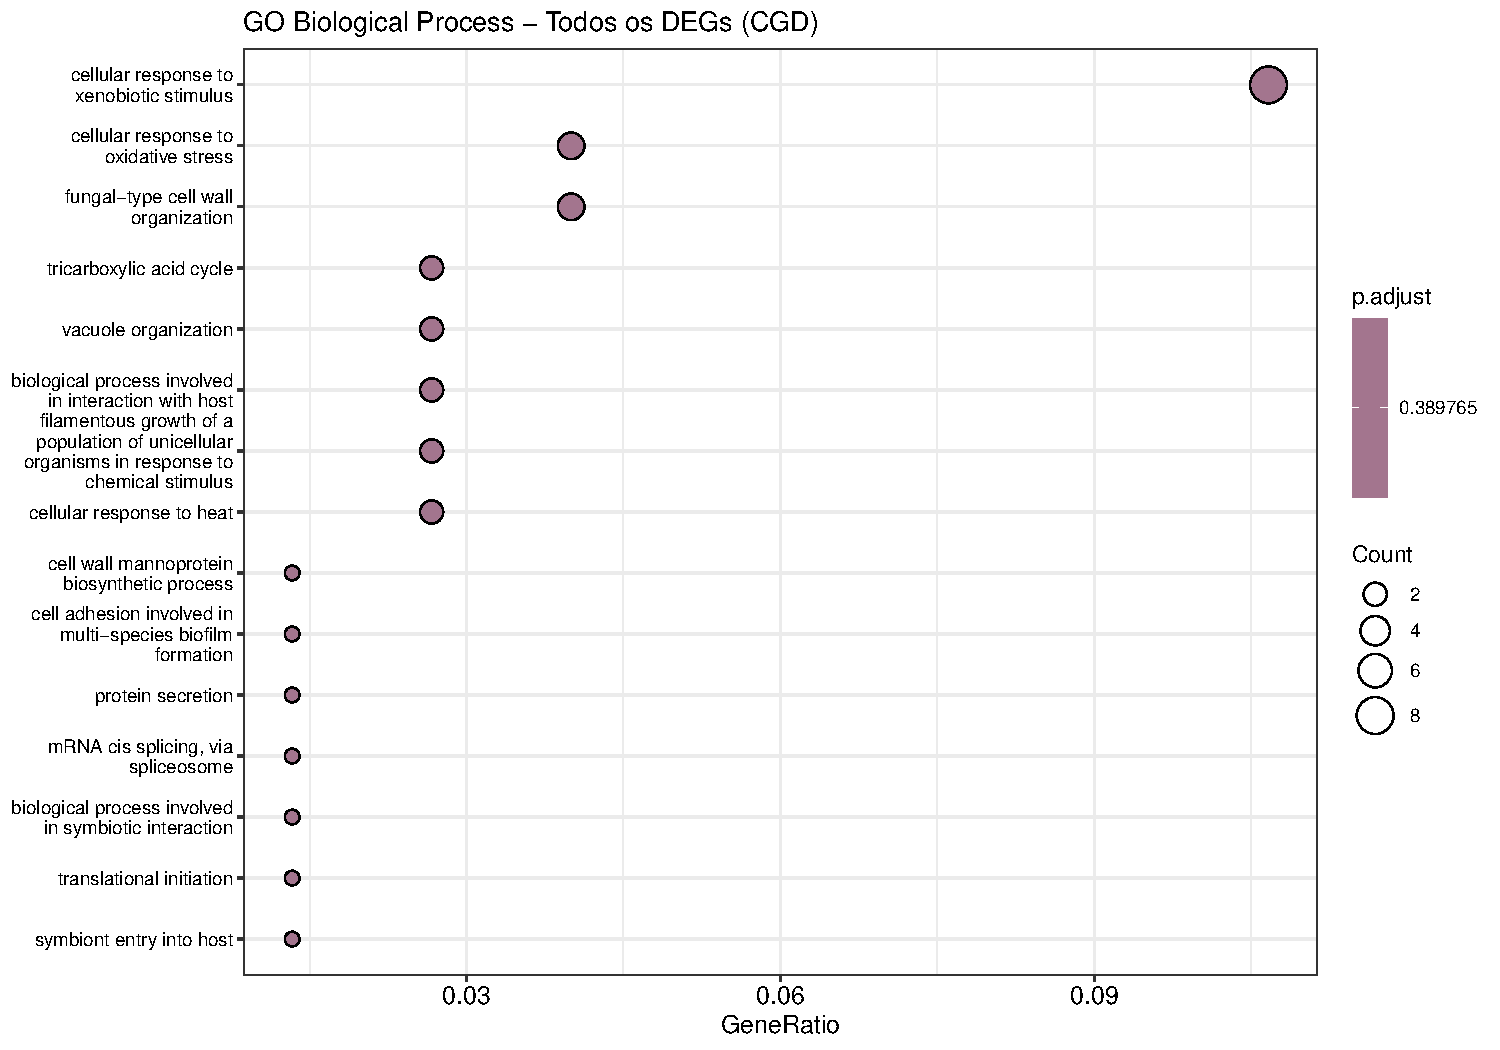
\includegraphics[keepaspectratio]{analysis/04_downstream_analyses_files/figure-pdf/unnamed-chunk-19-1.pdf}}

\subsection{Barplot Bidirecional --- GO BP UP
vs.~DOWN}\label{barplot-bidirecional-go-bp-up-vs.-down}

\begin{Shaded}
\begin{Highlighting}[]
\CommentTok{\# Extrair resultados de UP e DOWN}
\NormalTok{df\_go\_up }\OtherTok{\textless{}{-}} \ControlFlowTok{if}\NormalTok{ (}\SpecialCharTok{!}\FunctionTok{is.null}\NormalTok{(go\_up) }\SpecialCharTok{\&\&} \FunctionTok{nrow}\NormalTok{(}\FunctionTok{as.data.frame}\NormalTok{(go\_up)) }\SpecialCharTok{\textgreater{}} \DecValTok{0}\NormalTok{) \{}
  \FunctionTok{as.data.frame}\NormalTok{(go\_up) }\SpecialCharTok{\%\textgreater{}\%} \FunctionTok{mutate}\NormalTok{(}\AttributeTok{Direction =} \StringTok{"Upregulated"}\NormalTok{, }\AttributeTok{Count\_dir =}\NormalTok{ Count)}
\NormalTok{\} }\ControlFlowTok{else}\NormalTok{ \{ }\FunctionTok{data.frame}\NormalTok{() \}}

\NormalTok{df\_go\_down }\OtherTok{\textless{}{-}} \ControlFlowTok{if}\NormalTok{ (}\SpecialCharTok{!}\FunctionTok{is.null}\NormalTok{(go\_down) }\SpecialCharTok{\&\&} \FunctionTok{nrow}\NormalTok{(}\FunctionTok{as.data.frame}\NormalTok{(go\_down)) }\SpecialCharTok{\textgreater{}} \DecValTok{0}\NormalTok{) \{}
  \FunctionTok{as.data.frame}\NormalTok{(go\_down) }\SpecialCharTok{\%\textgreater{}\%} \FunctionTok{mutate}\NormalTok{(}\AttributeTok{Direction =} \StringTok{"Downregulated"}\NormalTok{, }\AttributeTok{Count\_dir =} \SpecialCharTok{{-}}\NormalTok{Count)}
\NormalTok{\} }\ControlFlowTok{else}\NormalTok{ \{ }\FunctionTok{data.frame}\NormalTok{() \}}

\ControlFlowTok{if}\NormalTok{ (}\FunctionTok{nrow}\NormalTok{(df\_go\_up) }\SpecialCharTok{\textgreater{}} \DecValTok{0} \SpecialCharTok{||} \FunctionTok{nrow}\NormalTok{(df\_go\_down) }\SpecialCharTok{\textgreater{}} \DecValTok{0}\NormalTok{) \{}
\NormalTok{  df\_go\_bidir }\OtherTok{\textless{}{-}} \FunctionTok{bind\_rows}\NormalTok{(}
\NormalTok{    df\_go\_up }\SpecialCharTok{\%\textgreater{}\%} \FunctionTok{head}\NormalTok{(}\DecValTok{10}\NormalTok{),}
\NormalTok{    df\_go\_down }\SpecialCharTok{\%\textgreater{}\%} \FunctionTok{head}\NormalTok{(}\DecValTok{10}\NormalTok{)}
\NormalTok{  )}

  \FunctionTok{ggplot}\NormalTok{(df\_go\_bidir, }\FunctionTok{aes}\NormalTok{(}\AttributeTok{x =}\NormalTok{ Count\_dir, }\AttributeTok{y =} \FunctionTok{reorder}\NormalTok{(Description, Count\_dir), }\AttributeTok{fill =}\NormalTok{ Direction)) }\SpecialCharTok{+}
    \FunctionTok{geom\_col}\NormalTok{(}\AttributeTok{width =} \FloatTok{0.7}\NormalTok{) }\SpecialCharTok{+}
    \FunctionTok{scale\_fill\_manual}\NormalTok{(}\AttributeTok{values =} \FunctionTok{c}\NormalTok{(}\StringTok{"Upregulated"} \OtherTok{=} \StringTok{"\#E31A1C"}\NormalTok{, }\StringTok{"Downregulated"} \OtherTok{=} \StringTok{"\#1F78B4"}\NormalTok{)) }\SpecialCharTok{+}
    \FunctionTok{geom\_vline}\NormalTok{(}\AttributeTok{xintercept =} \DecValTok{0}\NormalTok{, }\AttributeTok{linewidth =} \FloatTok{0.5}\NormalTok{) }\SpecialCharTok{+}
    \FunctionTok{labs}\NormalTok{(}\AttributeTok{title =} \StringTok{"GO Biological Process — UP vs. DOWN (CGD)"}\NormalTok{,}
         \AttributeTok{x =} \StringTok{"Número de Genes"}\NormalTok{, }\AttributeTok{y =} \ConstantTok{NULL}\NormalTok{, }\AttributeTok{fill =} \StringTok{"Regulação"}\NormalTok{) }\SpecialCharTok{+}
    \FunctionTok{theme\_minimal}\NormalTok{(}\AttributeTok{base\_size =} \DecValTok{13}\NormalTok{) }\SpecialCharTok{+}
    \FunctionTok{theme}\NormalTok{(}\AttributeTok{plot.title =} \FunctionTok{element\_text}\NormalTok{(}\AttributeTok{hjust =} \FloatTok{0.5}\NormalTok{, }\AttributeTok{face =} \StringTok{"bold"}\NormalTok{),}
          \AttributeTok{axis.text.y =} \FunctionTok{element\_text}\NormalTok{(}\AttributeTok{size =} \DecValTok{9}\NormalTok{),}
          \AttributeTok{legend.position =} \StringTok{"bottom"}\NormalTok{)}
\NormalTok{\} }\ControlFlowTok{else}\NormalTok{ \{}
  \FunctionTok{cat}\NormalTok{(}\StringTok{"Nenhum processo biológico enriquecido para gerar o barplot bidirecional.}\SpecialCharTok{\textbackslash{}n}\StringTok{"}\NormalTok{)}
\NormalTok{\}}
\end{Highlighting}
\end{Shaded}

\pandocbounded{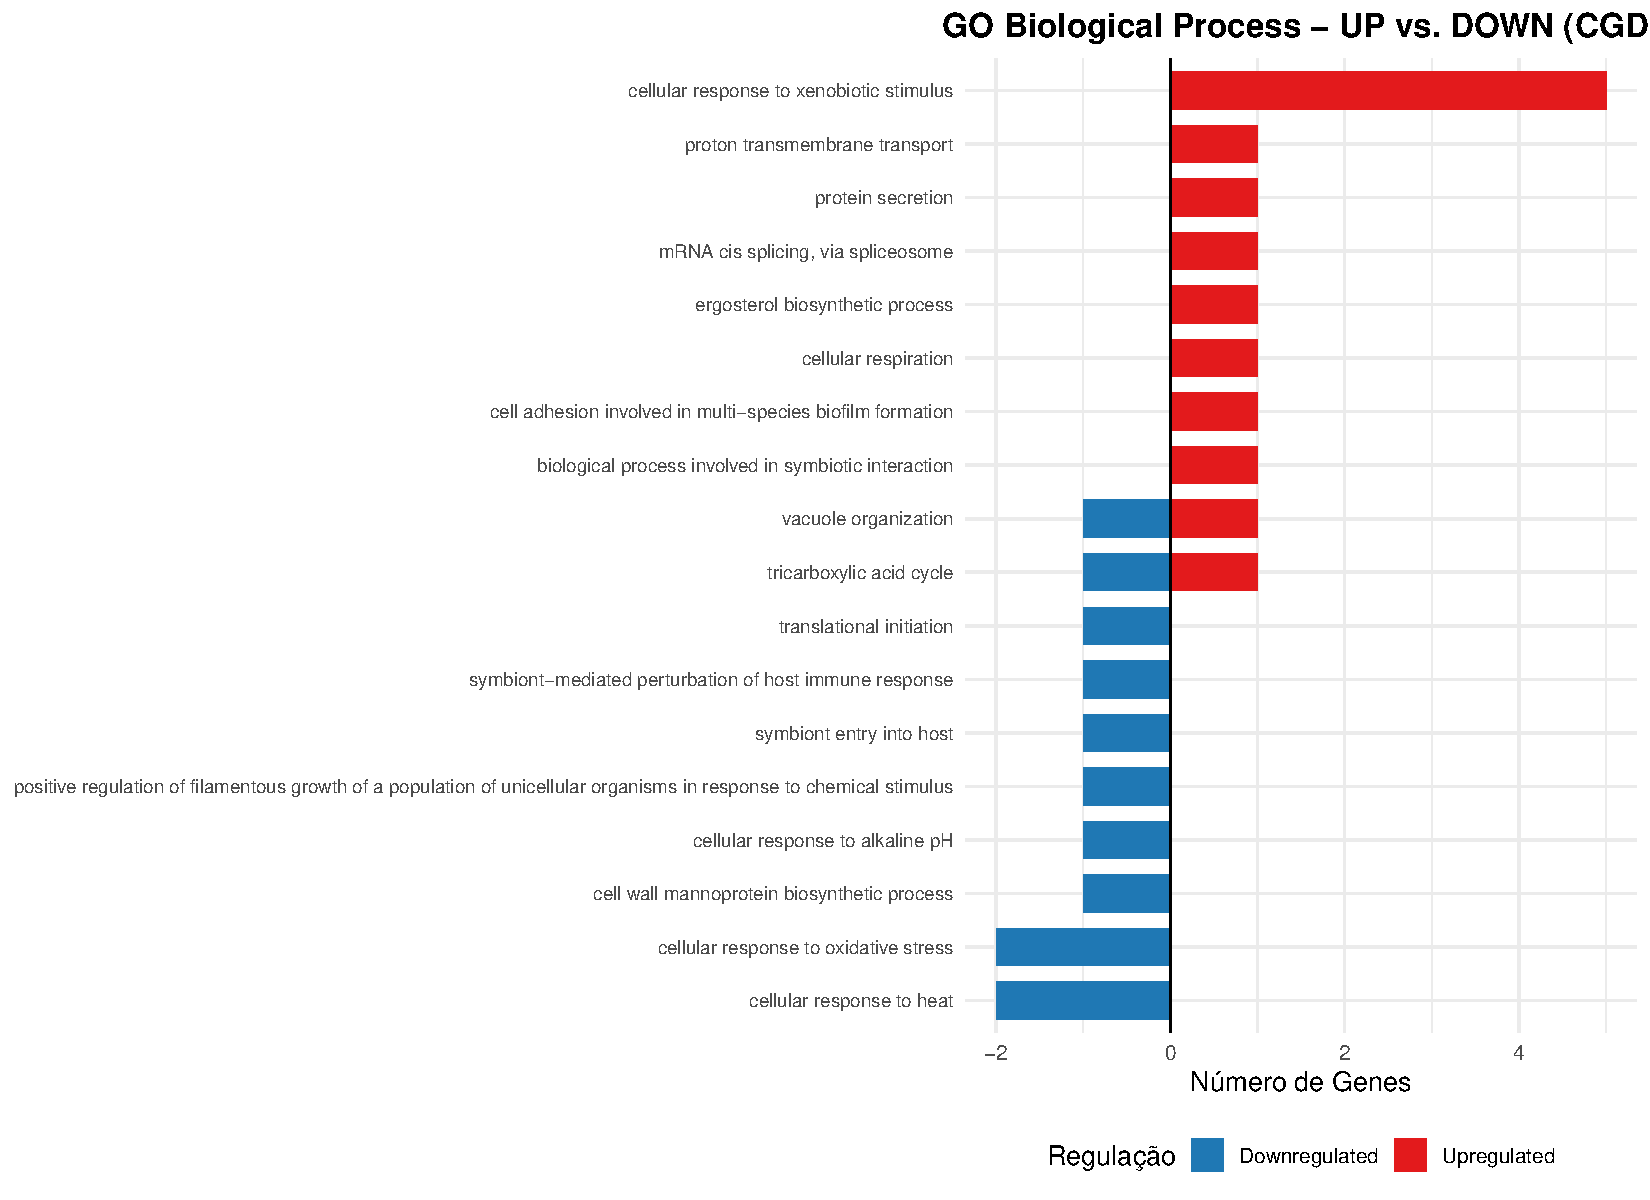
\includegraphics[keepaspectratio]{analysis/04_downstream_analyses_files/figure-pdf/unnamed-chunk-20-1.pdf}}

\subsection{Barplot --- GO BP Todos os
DEGs}\label{barplot-go-bp-todos-os-degs}

\begin{Shaded}
\begin{Highlighting}[]
\ControlFlowTok{if}\NormalTok{ (}\SpecialCharTok{!}\FunctionTok{is.null}\NormalTok{(go\_all) }\SpecialCharTok{\&\&} \FunctionTok{nrow}\NormalTok{(}\FunctionTok{as.data.frame}\NormalTok{(go\_all)) }\SpecialCharTok{\textgreater{}} \DecValTok{0}\NormalTok{) \{}
  \FunctionTok{barplot}\NormalTok{(go\_all,}
          \AttributeTok{showCategory =} \DecValTok{15}\NormalTok{,}
          \AttributeTok{title =} \StringTok{"GO Biological Process — Todos os DEGs (CGD)"}\NormalTok{,}
          \AttributeTok{color =} \StringTok{"p.adjust"}\NormalTok{) }\SpecialCharTok{+}
    \FunctionTok{theme}\NormalTok{(}\AttributeTok{axis.text.y =} \FunctionTok{element\_text}\NormalTok{(}\AttributeTok{size =} \DecValTok{9}\NormalTok{)) }\SpecialCharTok{+}
    \FunctionTok{scale\_fill\_gradient}\NormalTok{(}\AttributeTok{low =} \StringTok{"grey20"}\NormalTok{, }\AttributeTok{high =} \StringTok{"grey70"}\NormalTok{, }\AttributeTok{name =} \StringTok{"p{-}valor}\SpecialCharTok{\textbackslash{}n}\StringTok{ajustado"}\NormalTok{)}
\NormalTok{\} }\ControlFlowTok{else}\NormalTok{ \{}
  \FunctionTok{cat}\NormalTok{(}\StringTok{"Nenhum processo biológico enriquecido para todos os DEGs.}\SpecialCharTok{\textbackslash{}n}\StringTok{"}\NormalTok{)}
\NormalTok{\}}
\end{Highlighting}
\end{Shaded}

\pandocbounded{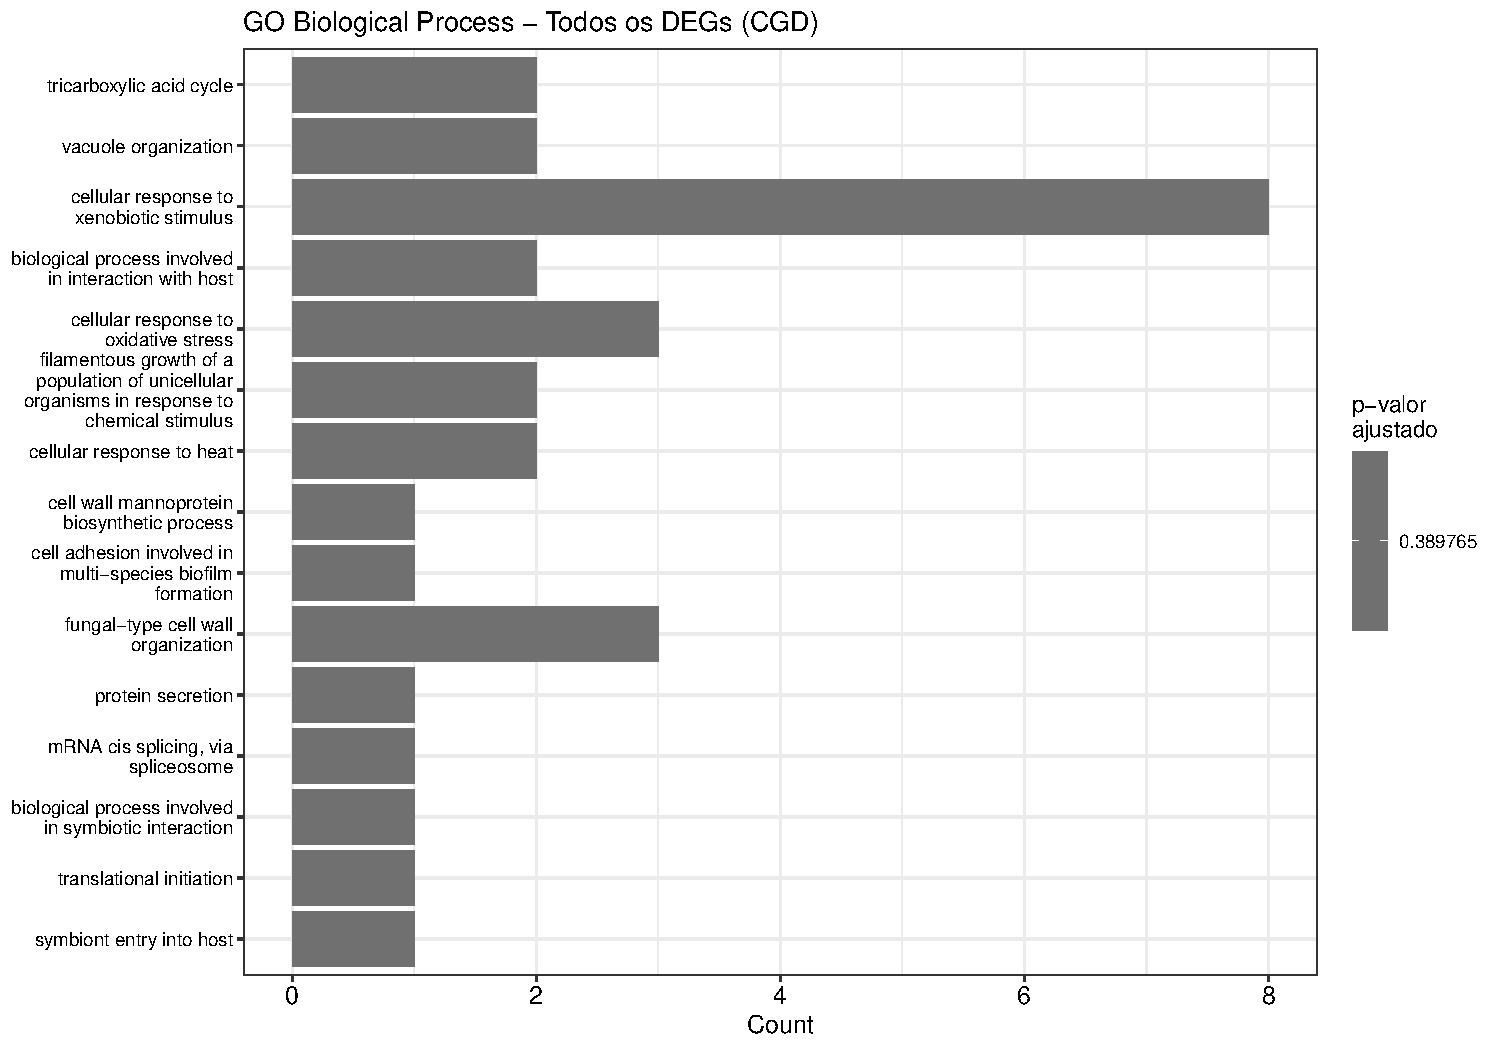
\includegraphics[keepaspectratio]{analysis/04_downstream_analyses_files/figure-pdf/unnamed-chunk-21-1.pdf}}

\begin{center}\rule{0.5\linewidth}{0.5pt}\end{center}

\section{8. Resumo e Interpretação}\label{resumo-e-interpretauxe7uxe3o}

\begin{Shaded}
\begin{Highlighting}[]
\FunctionTok{cat}\NormalTok{(}\StringTok{"=== Resumo do Enriquecimento Funcional ===}\SpecialCharTok{\textbackslash{}n\textbackslash{}n}\StringTok{"}\NormalTok{)}
\end{Highlighting}
\end{Shaded}

\begin{verbatim}
=== Resumo do Enriquecimento Funcional ===
\end{verbatim}

\begin{Shaded}
\begin{Highlighting}[]
\FunctionTok{cat}\NormalTok{(}\StringTok{"Genes UP:"}\NormalTok{, }\FunctionTok{length}\NormalTok{(genes\_up), }\StringTok{"| DOWN:"}\NormalTok{, }\FunctionTok{length}\NormalTok{(genes\_down),}
    \StringTok{"| Total:"}\NormalTok{, }\FunctionTok{length}\NormalTok{(genes\_all), }\StringTok{"}\SpecialCharTok{\textbackslash{}n\textbackslash{}n}\StringTok{"}\NormalTok{)}
\end{Highlighting}
\end{Shaded}

\begin{verbatim}
Genes UP: 40 | DOWN: 35 | Total: 75 
\end{verbatim}

\begin{Shaded}
\begin{Highlighting}[]
\FunctionTok{cat}\NormalTok{(}\StringTok{"{-}{-}{-} KEGG {-}{-}{-}}\SpecialCharTok{\textbackslash{}n}\StringTok{"}\NormalTok{)}
\end{Highlighting}
\end{Shaded}

\begin{verbatim}
--- KEGG ---
\end{verbatim}

\begin{Shaded}
\begin{Highlighting}[]
\FunctionTok{cat}\NormalTok{(}\StringTok{"  UP:   "}\NormalTok{)}
\end{Highlighting}
\end{Shaded}

\begin{verbatim}
  UP:   
\end{verbatim}

\begin{Shaded}
\begin{Highlighting}[]
\ControlFlowTok{if}\NormalTok{ (}\SpecialCharTok{!}\FunctionTok{is.null}\NormalTok{(kegg\_up) }\SpecialCharTok{\&\&} \FunctionTok{nrow}\NormalTok{(}\FunctionTok{as.data.frame}\NormalTok{(kegg\_up)) }\SpecialCharTok{\textgreater{}} \DecValTok{0}\NormalTok{) \{}
  \FunctionTok{cat}\NormalTok{(}\FunctionTok{nrow}\NormalTok{(}\FunctionTok{as.data.frame}\NormalTok{(kegg\_up)), }\StringTok{"vias}\SpecialCharTok{\textbackslash{}n}\StringTok{"}\NormalTok{)}
\NormalTok{\} }\ControlFlowTok{else}\NormalTok{ \{ }\FunctionTok{cat}\NormalTok{(}\StringTok{"nenhuma via}\SpecialCharTok{\textbackslash{}n}\StringTok{"}\NormalTok{) \}}
\end{Highlighting}
\end{Shaded}

\begin{verbatim}
22 vias
\end{verbatim}

\begin{Shaded}
\begin{Highlighting}[]
\FunctionTok{cat}\NormalTok{(}\StringTok{"  DOWN: "}\NormalTok{)}
\end{Highlighting}
\end{Shaded}

\begin{verbatim}
  DOWN: 
\end{verbatim}

\begin{Shaded}
\begin{Highlighting}[]
\ControlFlowTok{if}\NormalTok{ (}\SpecialCharTok{!}\FunctionTok{is.null}\NormalTok{(kegg\_down) }\SpecialCharTok{\&\&} \FunctionTok{nrow}\NormalTok{(}\FunctionTok{as.data.frame}\NormalTok{(kegg\_down)) }\SpecialCharTok{\textgreater{}} \DecValTok{0}\NormalTok{) \{}
  \FunctionTok{cat}\NormalTok{(}\FunctionTok{nrow}\NormalTok{(}\FunctionTok{as.data.frame}\NormalTok{(kegg\_down)), }\StringTok{"vias}\SpecialCharTok{\textbackslash{}n}\StringTok{"}\NormalTok{)}
\NormalTok{\} }\ControlFlowTok{else}\NormalTok{ \{ }\FunctionTok{cat}\NormalTok{(}\StringTok{"nenhuma via}\SpecialCharTok{\textbackslash{}n}\StringTok{"}\NormalTok{) \}}
\end{Highlighting}
\end{Shaded}

\begin{verbatim}
22 vias
\end{verbatim}

\begin{Shaded}
\begin{Highlighting}[]
\FunctionTok{cat}\NormalTok{(}\StringTok{"  ALL:  "}\NormalTok{)}
\end{Highlighting}
\end{Shaded}

\begin{verbatim}
  ALL:  
\end{verbatim}

\begin{Shaded}
\begin{Highlighting}[]
\ControlFlowTok{if}\NormalTok{ (}\SpecialCharTok{!}\FunctionTok{is.null}\NormalTok{(kegg\_all) }\SpecialCharTok{\&\&} \FunctionTok{nrow}\NormalTok{(}\FunctionTok{as.data.frame}\NormalTok{(kegg\_all)) }\SpecialCharTok{\textgreater{}} \DecValTok{0}\NormalTok{) \{}
  \FunctionTok{cat}\NormalTok{(}\FunctionTok{nrow}\NormalTok{(}\FunctionTok{as.data.frame}\NormalTok{(kegg\_all)), }\StringTok{"vias}\SpecialCharTok{\textbackslash{}n}\StringTok{"}\NormalTok{)}
\NormalTok{\} }\ControlFlowTok{else}\NormalTok{ \{ }\FunctionTok{cat}\NormalTok{(}\StringTok{"nenhuma via}\SpecialCharTok{\textbackslash{}n}\StringTok{"}\NormalTok{) \}}
\end{Highlighting}
\end{Shaded}

\begin{verbatim}
28 vias
\end{verbatim}

\begin{Shaded}
\begin{Highlighting}[]
\FunctionTok{cat}\NormalTok{(}\StringTok{"}\SpecialCharTok{\textbackslash{}n}\StringTok{{-}{-}{-} GO Biological Process (CGD) {-}{-}{-}}\SpecialCharTok{\textbackslash{}n}\StringTok{"}\NormalTok{)}
\end{Highlighting}
\end{Shaded}

\begin{verbatim}

--- GO Biological Process (CGD) ---
\end{verbatim}

\begin{Shaded}
\begin{Highlighting}[]
\FunctionTok{cat}\NormalTok{(}\StringTok{"  UP:   "}\NormalTok{)}
\end{Highlighting}
\end{Shaded}

\begin{verbatim}
  UP:   
\end{verbatim}

\begin{Shaded}
\begin{Highlighting}[]
\ControlFlowTok{if}\NormalTok{ (}\SpecialCharTok{!}\FunctionTok{is.null}\NormalTok{(go\_up) }\SpecialCharTok{\&\&} \FunctionTok{nrow}\NormalTok{(}\FunctionTok{as.data.frame}\NormalTok{(go\_up)) }\SpecialCharTok{\textgreater{}} \DecValTok{0}\NormalTok{) \{}
  \FunctionTok{cat}\NormalTok{(}\FunctionTok{nrow}\NormalTok{(}\FunctionTok{as.data.frame}\NormalTok{(go\_up)), }\StringTok{"termos}\SpecialCharTok{\textbackslash{}n}\StringTok{"}\NormalTok{)}
\NormalTok{\} }\ControlFlowTok{else}\NormalTok{ \{ }\FunctionTok{cat}\NormalTok{(}\StringTok{"nenhum termo}\SpecialCharTok{\textbackslash{}n}\StringTok{"}\NormalTok{) \}}
\end{Highlighting}
\end{Shaded}

\begin{verbatim}
28 termos
\end{verbatim}

\begin{Shaded}
\begin{Highlighting}[]
\FunctionTok{cat}\NormalTok{(}\StringTok{"  DOWN: "}\NormalTok{)}
\end{Highlighting}
\end{Shaded}

\begin{verbatim}
  DOWN: 
\end{verbatim}

\begin{Shaded}
\begin{Highlighting}[]
\ControlFlowTok{if}\NormalTok{ (}\SpecialCharTok{!}\FunctionTok{is.null}\NormalTok{(go\_down) }\SpecialCharTok{\&\&} \FunctionTok{nrow}\NormalTok{(}\FunctionTok{as.data.frame}\NormalTok{(go\_down)) }\SpecialCharTok{\textgreater{}} \DecValTok{0}\NormalTok{) \{}
  \FunctionTok{cat}\NormalTok{(}\FunctionTok{nrow}\NormalTok{(}\FunctionTok{as.data.frame}\NormalTok{(go\_down)), }\StringTok{"termos}\SpecialCharTok{\textbackslash{}n}\StringTok{"}\NormalTok{)}
\NormalTok{\} }\ControlFlowTok{else}\NormalTok{ \{ }\FunctionTok{cat}\NormalTok{(}\StringTok{"nenhum termo}\SpecialCharTok{\textbackslash{}n}\StringTok{"}\NormalTok{) \}}
\end{Highlighting}
\end{Shaded}

\begin{verbatim}
19 termos
\end{verbatim}

\begin{Shaded}
\begin{Highlighting}[]
\FunctionTok{cat}\NormalTok{(}\StringTok{"  ALL:  "}\NormalTok{)}
\end{Highlighting}
\end{Shaded}

\begin{verbatim}
  ALL:  
\end{verbatim}

\begin{Shaded}
\begin{Highlighting}[]
\ControlFlowTok{if}\NormalTok{ (}\SpecialCharTok{!}\FunctionTok{is.null}\NormalTok{(go\_all) }\SpecialCharTok{\&\&} \FunctionTok{nrow}\NormalTok{(}\FunctionTok{as.data.frame}\NormalTok{(go\_all)) }\SpecialCharTok{\textgreater{}} \DecValTok{0}\NormalTok{) \{}
  \FunctionTok{cat}\NormalTok{(}\FunctionTok{nrow}\NormalTok{(}\FunctionTok{as.data.frame}\NormalTok{(go\_all)), }\StringTok{"termos}\SpecialCharTok{\textbackslash{}n}\StringTok{"}\NormalTok{)}
\NormalTok{\} }\ControlFlowTok{else}\NormalTok{ \{ }\FunctionTok{cat}\NormalTok{(}\StringTok{"nenhum termo}\SpecialCharTok{\textbackslash{}n}\StringTok{"}\NormalTok{) \}}
\end{Highlighting}
\end{Shaded}

\begin{verbatim}
32 termos
\end{verbatim}

\textbf{Identificamos quais vias biológicas estão enriquecidas entre os
genes diferencialmente expressos da \emph{Candida albicans}. Mas como
esses genes se relacionam entre si? Será que as proteínas codificadas
por eles interagem fisicamente ou funcionam nos mesmos processos? Para
responder a essas perguntas, vamos construir uma rede de interação
proteína-proteína (PPI).}

\begin{center}\rule{0.5\linewidth}{0.5pt}\end{center}

\bookmarksetup{startatroot}

\chapter{Redes de Interação Proteína-Proteína
(PPI)}\label{redes-de-interauxe7uxe3o-proteuxedna-proteuxedna-ppi}

Uma lista de genes diferencialmente expressos nos diz \textbf{quais}
genes mudaram. O enriquecimento funcional nos diz \textbf{em quais vias}
esses genes participam. Mas nenhuma dessas análises nos mostra
\textbf{como} os produtos desses genes se relacionam entre si. É
exatamente essa lacuna que as redes de interação proteína-proteína (PPI)
preenchem.

Uma rede PPI é um grafo onde cada \textbf{nó} representa uma proteína e
cada \textbf{aresta} conecta duas proteínas que possuem alguma relação
funcional ou física documentada. Ao mapear nossos genes diferencialmente
expressos nessa rede.

\section{9. O Banco de Dados STRING}\label{o-banco-de-dados-string}

O \href{https://string-db.org/}{STRING (Search Tool for the Retrieval of
Interacting Genes/Proteins)} é o maior banco de dados público de
interações proteicas, cobrindo mais de 14.000 organismos. Um ponto
crucial é entender que o STRING \textbf{não armazena apenas interações
físicas diretas} (como ligações proteína-proteína demonstradas por
co-imunoprecipitação). Ele integra \textbf{múltiplas fontes de
evidência} para inferir \textbf{associações funcionais} entre proteínas:

{\def\LTcaptype{none} % do not increment counter
\begin{longtable}[]{@{}
  >{\raggedright\arraybackslash}p{(\linewidth - 4\tabcolsep) * \real{0.3333}}
  >{\raggedright\arraybackslash}p{(\linewidth - 4\tabcolsep) * \real{0.3333}}
  >{\raggedright\arraybackslash}p{(\linewidth - 4\tabcolsep) * \real{0.3333}}@{}}
\toprule\noalign{}
\begin{minipage}[b]{\linewidth}\raggedright
Canal de Evidência
\end{minipage} & \begin{minipage}[b]{\linewidth}\raggedright
Coluna
\end{minipage} & \begin{minipage}[b]{\linewidth}\raggedright
O que mede
\end{minipage} \\
\midrule\noalign{}
\endhead
\bottomrule\noalign{}
\endlastfoot
\textbf{Vizinhança genômica} & \texttt{nscore} & Genes fisicamente
próximos no genoma tendem a ser funcionalmente relacionados \\
\textbf{Fusão gênica} & \texttt{fscore} & Genes que aparecem fundidos em
outros organismos provavelmente interagem \\
\textbf{Co-ocorrência filogenética} & \texttt{pscore} & Proteínas que
co-evoluem (presentes/ausentes juntas em espécies) \\
\textbf{Co-expressão} & \texttt{ascore} & Genes com padrões de expressão
similares em múltiplos experimentos \\
\textbf{Evidência experimental} & \texttt{escore} & Interações
demonstradas por ensaios bioquímicos (Y2H, AP-MS, etc.) \\
\textbf{Bancos de dados curados} & \texttt{dscore} & Interações
registradas em bancos curados (KEGG, Reactome, BioCyc, etc.) \\
\textbf{Text mining} & \texttt{tscore} & Co-menção de proteínas na
literatura científica \\
\end{longtable}
}

Cada canal produz um \textbf{escore} entre 0 e 1 que indica a confiança
daquela evidência para um dado par de proteínas. O STRING combina esses
escores em um \textbf{escore combinado} usando uma fórmula
probabilística que evita dupla contagem.

\begin{tcolorbox}[enhanced jigsaw, arc=.35mm, bottomrule=.15mm, bottomtitle=1mm, breakable, colback=white, colbacktitle=quarto-callout-important-color!10!white, colframe=quarto-callout-important-color-frame, coltitle=black, left=2mm, leftrule=.75mm, opacityback=0, opacitybacktitle=0.6, rightrule=.15mm, title=\textcolor{quarto-callout-important-color}{\faExclamation}\hspace{0.5em}{Interações ≠ Interações Físicas}, titlerule=0mm, toprule=.15mm, toptitle=1mm]

É fundamental entender que o termo ``interação'' no STRING é mais amplo
do que interação física direta. Quando dizemos que duas proteínas
``interagem'' no STRING, estamos dizendo que há \textbf{evidência de
associação funcional}, elas podem participar do mesmo complexo, da mesma
via metabólica, ou serem co-reguladas, sem necessariamente se tocarem
fisicamente. Por isso, o termo mais preciso é \textbf{associação
funcional}.

\end{tcolorbox}

\begin{tcolorbox}[enhanced jigsaw, arc=.35mm, bottomrule=.15mm, bottomtitle=1mm, breakable, colback=white, colbacktitle=quarto-callout-note-color!10!white, colframe=quarto-callout-note-color-frame, coltitle=black, left=2mm, leftrule=.75mm, opacityback=0, opacitybacktitle=0.6, rightrule=.15mm, title=\textcolor{quarto-callout-note-color}{\faInfo}\hspace{0.5em}{Ponto Importante --- Bancos de Dados Curados e Organismos Não-Modelo}, titlerule=0mm, toprule=.15mm, toptitle=1mm]

Assim como vimos na análise de enriquecimento funcional, a qualidade dos
resultados de redes PPI depende diretamente da \textbf{completude do
banco de dados para o organismo estudado}. Para organismos-modelo como
\emph{Homo sapiens} e \emph{Saccharomyces cerevisiae}, o STRING possui
milhares de interações experimentalmente validadas. Para \emph{Candida
albicans}, a cobertura é menor, muitas interações são inferidas
computacionalmente a partir de ortologia com \emph{S. cerevisiae} ou por
text mining. Mesmo assim, o STRING suporta \emph{C. albicans} SC5314
nativamente (identificador taxonômico \textbf{237561}), o que nos
permite consultar a base diretamente.

\end{tcolorbox}

\section{10. Carregando os Pacotes}\label{carregando-os-pacotes-2}

\begin{Shaded}
\begin{Highlighting}[]
\FunctionTok{suppressPackageStartupMessages}\NormalTok{(\{}
  \FunctionTok{library}\NormalTok{(RCurl)}
  \FunctionTok{library}\NormalTok{(igraph)}
  \FunctionTok{library}\NormalTok{(ggraph)}
  \FunctionTok{library}\NormalTok{(ggplot2)}
  \FunctionTok{library}\NormalTok{(dplyr)}
  \FunctionTok{library}\NormalTok{(readr)}
  \FunctionTok{library}\NormalTok{(tibble)}
  \FunctionTok{library}\NormalTok{(scales)}
\NormalTok{\})}
\end{Highlighting}
\end{Shaded}

\section{11. Preparando a Lista de
Genes}\label{preparando-a-lista-de-genes}

Vamos recuperar nossos resultados de expressão diferencial e preparar a
lista de genes que será submetida ao STRING. O STRING não reconhece
diretamente os identificadores do Ensembl Fungi (ex:
\texttt{C1\_00210C\_A}). Para \emph{C. albicans}, o STRING utiliza os
identificadores no formato \texttt{CAALFM\_} (ex:
\texttt{CAALFM\_C100210CA}), que são os mesmos usados pelo CGD e pelo
KEGG. Felizmente, já construímos o dicionário de conversão
(\texttt{ensembl\_to\_kegg}) na seção anterior:

\begin{Shaded}
\begin{Highlighting}[]
\CommentTok{\# Carregar resultados da expressão diferencial}
\NormalTok{res\_dge }\OtherTok{\textless{}{-}} \FunctionTok{readRDS}\NormalTok{(here}\SpecialCharTok{::}\FunctionTok{here}\NormalTok{(}\StringTok{"data/DGE/res\_dge.rds"}\NormalTok{))}

\CommentTok{\# Selecionar apenas os genes significativos (DEGs)}
\NormalTok{res\_dge\_signif }\OtherTok{\textless{}{-}}\NormalTok{ res\_dge }\SpecialCharTok{\%\textgreater{}\%}
  \FunctionTok{filter}\NormalTok{(signif }\SpecialCharTok{!=} \StringTok{"Not significant"}\NormalTok{)}

\NormalTok{genes\_deg }\OtherTok{\textless{}{-}} \FunctionTok{rownames}\NormalTok{(res\_dge\_signif)}

\CommentTok{\# Converter Ensembl IDs para o formato CAALFM\_ usando o dicionário da seção 4}
\NormalTok{genes\_deg\_caalfm }\OtherTok{\textless{}{-}} \FunctionTok{unname}\NormalTok{(ensembl\_to\_kegg[genes\_deg[genes\_deg }\SpecialCharTok{\%in\%} \FunctionTok{names}\NormalTok{(ensembl\_to\_kegg)]])}

\CommentTok{\# Criar dicionário reverso para mapear de volta}
\NormalTok{caalfm\_to\_ensembl }\OtherTok{\textless{}{-}} \FunctionTok{setNames}\NormalTok{(}\FunctionTok{names}\NormalTok{(ensembl\_to\_kegg), }\FunctionTok{unname}\NormalTok{(ensembl\_to\_kegg))}

\FunctionTok{cat}\NormalTok{(}\StringTok{"Total de DEGs:"}\NormalTok{, }\FunctionTok{length}\NormalTok{(genes\_deg), }\StringTok{"}\SpecialCharTok{\textbackslash{}n}\StringTok{"}\NormalTok{)}
\end{Highlighting}
\end{Shaded}

\begin{verbatim}
Total de DEGs: 75 
\end{verbatim}

\begin{Shaded}
\begin{Highlighting}[]
\FunctionTok{cat}\NormalTok{(}\StringTok{"DEGs com ID CAALFM\_ mapeado:"}\NormalTok{, }\FunctionTok{length}\NormalTok{(genes\_deg\_caalfm), }\StringTok{"}\SpecialCharTok{\textbackslash{}n}\StringTok{"}\NormalTok{)}
\end{Highlighting}
\end{Shaded}

\begin{verbatim}
DEGs com ID CAALFM_ mapeado: 75 
\end{verbatim}

\begin{tcolorbox}[enhanced jigsaw, arc=.35mm, bottomrule=.15mm, bottomtitle=1mm, breakable, colback=white, colbacktitle=quarto-callout-note-color!10!white, colframe=quarto-callout-note-color-frame, coltitle=black, left=2mm, leftrule=.75mm, opacityback=0, opacitybacktitle=0.6, rightrule=.15mm, title=\textcolor{quarto-callout-note-color}{\faInfo}\hspace{0.5em}{Ponto Importante --- Conversão de Identificadores}, titlerule=0mm, toprule=.15mm, toptitle=1mm]

A conversão entre Ensembl Fungi e CAALFM\_ segue uma regra simples: o ID
\texttt{C1\_00010W\_A} corresponde a \texttt{CAALFM\_C100010WA} (remoção
dos underscores e adição do prefixo). Essa é a mesma conversão que
fizemos para o KEGG na seção 4. Se um gene não possui correspondência no
dicionário, ele simplesmente não será incluído na rede.

\end{tcolorbox}

\section{12. Consultando o STRING via
API}\label{consultando-o-string-via-api}

O STRING disponibiliza uma \href{https://string-db.org/help/api/}{API
pública} que permite realizar consultas programáticas. Vamos utilizá-la
para: (1) mapear nossos identificadores \texttt{CAALFM\_} para os
identificadores internos do STRING, e (2) obter a rede de interações
entre eles.

O identificador taxonômico da cepa SC5314 de \emph{C. albicans} no
STRING é \textbf{237561}.

\subsection{Mapeando os
identificadores}\label{mapeando-os-identificadores}

\begin{Shaded}
\begin{Highlighting}[]
\CommentTok{\# Concatenar os genes no formato CAALFM\_ para a requisição à API}
\NormalTok{genes\_concatenado }\OtherTok{\textless{}{-}} \FunctionTok{paste0}\NormalTok{(genes\_deg\_caalfm, }\AttributeTok{collapse =} \StringTok{"\%0d"}\NormalTok{)}

\CommentTok{\# Requisição para mapear nossos IDs para os IDs do STRING}
\NormalTok{req\_map }\OtherTok{\textless{}{-}}\NormalTok{ RCurl}\SpecialCharTok{::}\FunctionTok{postForm}\NormalTok{(}
  \StringTok{"https://string{-}db.org/api/tsv/get\_string\_ids"}\NormalTok{,}
  \AttributeTok{identifiers =}\NormalTok{ genes\_concatenado,}
  \AttributeTok{echo\_query =} \StringTok{"1"}\NormalTok{,}
  \AttributeTok{species =} \StringTok{"237561"}  \CommentTok{\# C. albicans SC5314}
\NormalTok{)}

\NormalTok{map\_ids }\OtherTok{\textless{}{-}} \FunctionTok{read.table}\NormalTok{(}\AttributeTok{text =}\NormalTok{ req\_map, }\AttributeTok{sep =} \StringTok{"}\SpecialCharTok{\textbackslash{}t}\StringTok{"}\NormalTok{, }\AttributeTok{header =} \ConstantTok{TRUE}\NormalTok{, }\AttributeTok{quote =} \StringTok{""}\NormalTok{)}

\FunctionTok{cat}\NormalTok{(}\StringTok{"Genes mapeados no STRING:"}\NormalTok{, }\FunctionTok{nrow}\NormalTok{(map\_ids), }\StringTok{"de"}\NormalTok{, }\FunctionTok{length}\NormalTok{(genes\_deg\_caalfm), }\StringTok{"}\SpecialCharTok{\textbackslash{}n}\StringTok{"}\NormalTok{)}
\end{Highlighting}
\end{Shaded}

\begin{verbatim}
Genes mapeados no STRING: 70 de 75 
\end{verbatim}

\subsection{Obtendo a rede de
interações}\label{obtendo-a-rede-de-interauxe7uxf5es}

\begin{Shaded}
\begin{Highlighting}[]
\CommentTok{\# Concatenar os identificadores do STRING}
\NormalTok{genes\_string\_concatenado }\OtherTok{\textless{}{-}} \FunctionTok{paste0}\NormalTok{(}\FunctionTok{unique}\NormalTok{(map\_ids}\SpecialCharTok{$}\NormalTok{stringId), }\AttributeTok{collapse =} \StringTok{"\%0d"}\NormalTok{)}

\CommentTok{\# Requisição para o método \textquotesingle{}network\textquotesingle{}}
\NormalTok{req\_net }\OtherTok{\textless{}{-}}\NormalTok{ RCurl}\SpecialCharTok{::}\FunctionTok{postForm}\NormalTok{(}
  \StringTok{"https://string{-}db.org/api/tsv/network"}\NormalTok{,}
  \AttributeTok{identifiers =}\NormalTok{ genes\_string\_concatenado,}
  \AttributeTok{required\_score =} \StringTok{"0"}\NormalTok{,   }\CommentTok{\# Sem filtro mínimo (filtraremos depois)}
  \AttributeTok{species =} \StringTok{"237561"}
\NormalTok{)}

\NormalTok{int\_network }\OtherTok{\textless{}{-}} \FunctionTok{read.table}\NormalTok{(}\AttributeTok{text =}\NormalTok{ req\_net, }\AttributeTok{sep =} \StringTok{"}\SpecialCharTok{\textbackslash{}t}\StringTok{"}\NormalTok{, }\AttributeTok{header =} \ConstantTok{TRUE}\NormalTok{)}
\NormalTok{int\_network }\OtherTok{\textless{}{-}} \FunctionTok{unique}\NormalTok{(int\_network)}

\FunctionTok{cat}\NormalTok{(}\StringTok{"Interações brutas obtidas:"}\NormalTok{, }\FunctionTok{nrow}\NormalTok{(int\_network), }\StringTok{"}\SpecialCharTok{\textbackslash{}n}\StringTok{"}\NormalTok{)}
\end{Highlighting}
\end{Shaded}

\begin{verbatim}
Interações brutas obtidas: 237 
\end{verbatim}

\section{\texorpdfstring{13. Filtrando as Interações com
\texttt{combinescores}}{13. Filtrando as Interações com combinescores}}\label{filtrando-as-interauxe7uxf5es-com-combinescores}

As interações brutas incluem todas as fontes de evidência e todos os
níveis de confiança. Para obtermos uma rede de alta qualidade,
precisamos:

\begin{enumerate}
\def\labelenumi{\arabic{enumi}.}
\tightlist
\item
  \textbf{Selecionar os canais de evidência} mais confiáveis para o
  nosso contexto.
\item
  \textbf{Combinar os escores} desses canais usando a fórmula
  probabilística do STRING.
\item
  \textbf{Filtrar} pelo escore combinado mínimo.
\end{enumerate}

A função \texttt{combinescores} abaixo implementa exatamente esse
procedimento. Ela recebe a tabela de interações, seleciona os canais
desejados e calcula o escore combinado usando a fórmula:
\(1 - \prod_{i}(1 - S_i)\), onde \(S_i\) é o escore de cada canal. Essa
abordagem probabilística garante que \textbf{múltiplas fontes fracas de
evidência possam se somar} para produzir uma interação de alta
confiança.

\begin{Shaded}
\begin{Highlighting}[]
\CommentTok{\# Função para combinar escores de acordo com o algoritmo do STRING}
\NormalTok{combinescores }\OtherTok{\textless{}{-}} \ControlFlowTok{function}\NormalTok{(dat, }\AttributeTok{evidences =} \StringTok{"all"}\NormalTok{, }\AttributeTok{confLevel =} \FloatTok{0.4}\NormalTok{) \{}
  \ControlFlowTok{if}\NormalTok{ (evidences[}\DecValTok{1}\NormalTok{] }\SpecialCharTok{==} \StringTok{"all"}\NormalTok{) \{}
\NormalTok{    edat }\OtherTok{\textless{}{-}}\NormalTok{ dat[, }\SpecialCharTok{{-}}\FunctionTok{c}\NormalTok{(}\DecValTok{1}\NormalTok{, }\DecValTok{2}\NormalTok{, }\FunctionTok{ncol}\NormalTok{(dat))]}
\NormalTok{  \} }\ControlFlowTok{else}\NormalTok{ \{}
    \ControlFlowTok{if}\NormalTok{ (}\SpecialCharTok{!}\FunctionTok{all}\NormalTok{(evidences }\SpecialCharTok{\%in\%} \FunctionTok{colnames}\NormalTok{(dat))) \{}
      \FunctionTok{stop}\NormalTok{(}\StringTok{"ERRO: uma ou mais evidências não encontradas nas colunas dos dados!"}\NormalTok{)}
\NormalTok{    \}}
\NormalTok{    edat }\OtherTok{\textless{}{-}}\NormalTok{ dat[, evidences]}
\NormalTok{  \}}
  \CommentTok{\# Os escores do STRING vêm em escala 0{-}1000; converter para 0{-}1}
  \ControlFlowTok{if}\NormalTok{ (}\FunctionTok{any}\NormalTok{(edat }\SpecialCharTok{\textgreater{}} \DecValTok{1}\NormalTok{)) \{}
\NormalTok{    edat }\OtherTok{\textless{}{-}}\NormalTok{ edat }\SpecialCharTok{/} \DecValTok{1000}
\NormalTok{  \}}
  \CommentTok{\# Fórmula probabilística: 1 {-} prod(1 {-} Si)}
\NormalTok{  edat }\OtherTok{\textless{}{-}} \DecValTok{1} \SpecialCharTok{{-}}\NormalTok{ edat}
\NormalTok{  sc }\OtherTok{\textless{}{-}} \FunctionTok{apply}\NormalTok{(}\AttributeTok{X =}\NormalTok{ edat, }\AttributeTok{MARGIN =} \DecValTok{1}\NormalTok{, }\AttributeTok{FUN =} \ControlFlowTok{function}\NormalTok{(x) }\DecValTok{1} \SpecialCharTok{{-}} \FunctionTok{prod}\NormalTok{(x))}
\NormalTok{  dat }\OtherTok{\textless{}{-}} \FunctionTok{cbind}\NormalTok{(dat[, }\FunctionTok{c}\NormalTok{(}\DecValTok{1}\NormalTok{, }\DecValTok{2}\NormalTok{)], }\AttributeTok{combined\_score =}\NormalTok{ sc)}
\NormalTok{  idx }\OtherTok{\textless{}{-}}\NormalTok{ dat}\SpecialCharTok{$}\NormalTok{combined\_score }\SpecialCharTok{\textgreater{}=}\NormalTok{ confLevel}
\NormalTok{  dat }\OtherTok{\textless{}{-}}\NormalTok{ dat[idx, ]}
  \FunctionTok{return}\NormalTok{(dat)}
\NormalTok{\}}
\end{Highlighting}
\end{Shaded}

Vamos aplicar o filtro. Utilizaremos os canais de \textbf{co-expressão},
\textbf{evidência experimental} e \textbf{bancos de dados curados}.
Aqui, por motivos didáticos, vamos estabelecer um escore combinado
mínimo de \textbf{0.15} (baixa confiança):

\begin{Shaded}
\begin{Highlighting}[]
\CommentTok{\# Aplicar o filtro por canais e confiança mínima}
\NormalTok{int\_network\_filtered }\OtherTok{\textless{}{-}} \FunctionTok{combinescores}\NormalTok{(}
\NormalTok{  int\_network,}
  \AttributeTok{evidences =} \FunctionTok{c}\NormalTok{(}\StringTok{"ascore"}\NormalTok{, }\StringTok{"escore"}\NormalTok{, }\StringTok{"dscore"}\NormalTok{),}
  \AttributeTok{confLevel =} \FloatTok{0.15}
\NormalTok{)}

\FunctionTok{cat}\NormalTok{(}\StringTok{"Interações após filtro (confiança ≥ 0.15):"}\NormalTok{, }\FunctionTok{nrow}\NormalTok{(int\_network\_filtered), }\StringTok{"}\SpecialCharTok{\textbackslash{}n}\StringTok{"}\NormalTok{)}
\end{Highlighting}
\end{Shaded}

\begin{verbatim}
Interações após filtro (confiança ≥ 0.15): 157 
\end{verbatim}

\begin{tcolorbox}[enhanced jigsaw, arc=.35mm, bottomrule=.15mm, bottomtitle=1mm, breakable, colback=white, colbacktitle=quarto-callout-note-color!10!white, colframe=quarto-callout-note-color-frame, coltitle=black, left=2mm, leftrule=.75mm, opacityback=0, opacitybacktitle=0.6, rightrule=.15mm, title=\textcolor{quarto-callout-note-color}{\faInfo}\hspace{0.5em}{Ponto Importante --- Escolha do Threshold}, titlerule=0mm, toprule=.15mm, toptitle=1mm]

O STRING utiliza uma classificação de confiança para seus escores:

\begin{itemize}
\tightlist
\item
  \textbf{Low confidence:} \textgreater{} 0.15
\item
  \textbf{Medium confidence:} \textgreater{} 0.4
\item
  \textbf{High confidence:} \textgreater{} 0.7
\item
  \textbf{Highest confidence:} \textgreater{} 0.9
\end{itemize}

Para \emph{C. albicans}, um organismo com menos interações
experimentalmente validadas, utilizamos o threshold de \textbf{baixa
confiança (0.15)} de forma didática para obter uma rede com conexões
suficientes a fim de explorar e interpretar grafos durante a aula.
Diferentes escores devem ser empregados (como \textgreater{} 0.4 ou 0.7)
a depender do contexto e perguntas biológicas com intenção em dados com
nível maior de acurácia.

\end{tcolorbox}

\section{14. Construindo o Grafo com
igraph}\label{construindo-o-grafo-com-igraph}

Agora vamos transformar a tabela de interações filtrada em um
\textbf{objeto igraph} e anotar cada nó com as informações de expressão
diferencial (log2FC e significância):

\begin{Shaded}
\begin{Highlighting}[]
\CommentTok{\# Criar dataframe de anotação mapeando stringId → nomes preferenciais e IDs originais}
\NormalTok{ann }\OtherTok{\textless{}{-}} \FunctionTok{data.frame}\NormalTok{(}
  \AttributeTok{stringId =}\NormalTok{ map\_ids}\SpecialCharTok{$}\NormalTok{stringId,}
  \AttributeTok{gene\_name =}\NormalTok{ map\_ids}\SpecialCharTok{$}\NormalTok{preferredName,}
  \AttributeTok{query\_caalfm =}\NormalTok{ map\_ids}\SpecialCharTok{$}\NormalTok{queryItem,}
  \AttributeTok{stringsAsFactors =} \ConstantTok{FALSE}
\NormalTok{) }\SpecialCharTok{\%\textgreater{}\%}
  \FunctionTok{distinct}\NormalTok{(stringId, }\AttributeTok{.keep\_all =} \ConstantTok{TRUE}\NormalTok{) }\SpecialCharTok{\%\textgreater{}\%}
  \FunctionTok{mutate}\NormalTok{(}
    \CommentTok{\# Mapear CAALFM\_ de volta para Ensembl ID}
    \AttributeTok{ensembl\_id =}\NormalTok{ caalfm\_to\_ensembl[query\_caalfm]}
\NormalTok{  )}

\CommentTok{\# Substituir os stringIds pelos nomes dos genes na tabela de interações}
\NormalTok{int\_network\_named }\OtherTok{\textless{}{-}}\NormalTok{ int\_network\_filtered }\SpecialCharTok{\%\textgreater{}\%}
  \FunctionTok{mutate}\NormalTok{(}
    \AttributeTok{gene\_A =}\NormalTok{ ann}\SpecialCharTok{$}\NormalTok{gene\_name[}\FunctionTok{match}\NormalTok{(stringId\_A, ann}\SpecialCharTok{$}\NormalTok{stringId)],}
    \AttributeTok{gene\_B =}\NormalTok{ ann}\SpecialCharTok{$}\NormalTok{gene\_name[}\FunctionTok{match}\NormalTok{(stringId\_B, ann}\SpecialCharTok{$}\NormalTok{stringId)]}
\NormalTok{  ) }\SpecialCharTok{\%\textgreater{}\%}
  \FunctionTok{filter}\NormalTok{(}\SpecialCharTok{!}\FunctionTok{is.na}\NormalTok{(gene\_A), }\SpecialCharTok{!}\FunctionTok{is.na}\NormalTok{(gene\_B)) }\SpecialCharTok{\%\textgreater{}\%}
\NormalTok{  dplyr}\SpecialCharTok{::}\FunctionTok{select}\NormalTok{(gene\_A, gene\_B, combined\_score)}

\CommentTok{\# Criar objeto igraph (rede não direcionada)}
\NormalTok{g }\OtherTok{\textless{}{-}} \FunctionTok{graph\_from\_data\_frame}\NormalTok{(int\_network\_named, }\AttributeTok{directed =} \ConstantTok{FALSE}\NormalTok{)}

\CommentTok{\# Remover arestas duplicadas e auto{-}loops}
\NormalTok{g }\OtherTok{\textless{}{-}}\NormalTok{ igraph}\SpecialCharTok{::}\FunctionTok{simplify}\NormalTok{(g)}

\FunctionTok{cat}\NormalTok{(}\StringTok{"Rede construída:"}\NormalTok{, }\FunctionTok{vcount}\NormalTok{(g), }\StringTok{"nós,"}\NormalTok{, }\FunctionTok{ecount}\NormalTok{(g), }\StringTok{"arestas}\SpecialCharTok{\textbackslash{}n}\StringTok{"}\NormalTok{)}
\end{Highlighting}
\end{Shaded}

\begin{verbatim}
Rede construída: 64 nós, 157 arestas
\end{verbatim}

\subsection{Anotando os nós com informações de
expressão}\label{anotando-os-nuxf3s-com-informauxe7uxf5es-de-expressuxe3o}

\begin{Shaded}
\begin{Highlighting}[]
\CommentTok{\# Criar dicionário gene\_name → ensembl\_id}
\NormalTok{name\_to\_ensembl }\OtherTok{\textless{}{-}} \FunctionTok{setNames}\NormalTok{(ann}\SpecialCharTok{$}\NormalTok{ensembl\_id, ann}\SpecialCharTok{$}\NormalTok{gene\_name)}

\CommentTok{\# Para cada nó do grafo, buscar o Ensembl ID e depois as informações do DEG}
\NormalTok{node\_names }\OtherTok{\textless{}{-}} \FunctionTok{V}\NormalTok{(g)}\SpecialCharTok{$}\NormalTok{name}
\NormalTok{node\_ensembl }\OtherTok{\textless{}{-}}\NormalTok{ name\_to\_ensembl[node\_names]}

\CommentTok{\# Extrair log2FC e padj}
\NormalTok{node\_log2fc }\OtherTok{\textless{}{-}}\NormalTok{ res\_dge[node\_ensembl, }\StringTok{"log2FoldChange"}\NormalTok{]}
\NormalTok{node\_padj }\OtherTok{\textless{}{-}}\NormalTok{ res\_dge[node\_ensembl, }\StringTok{"padj"}\NormalTok{]}
\NormalTok{node\_signif }\OtherTok{\textless{}{-}}\NormalTok{ res\_dge[node\_ensembl, }\StringTok{"signif"}\NormalTok{]}

\CommentTok{\# Atribuir como atributos do grafo}
\FunctionTok{V}\NormalTok{(g)}\SpecialCharTok{$}\NormalTok{log2FC }\OtherTok{\textless{}{-}} \FunctionTok{ifelse}\NormalTok{(}\FunctionTok{is.na}\NormalTok{(node\_log2fc), }\DecValTok{0}\NormalTok{, node\_log2fc)}
\FunctionTok{V}\NormalTok{(g)}\SpecialCharTok{$}\NormalTok{padj }\OtherTok{\textless{}{-}} \FunctionTok{ifelse}\NormalTok{(}\FunctionTok{is.na}\NormalTok{(node\_padj), }\DecValTok{1}\NormalTok{, node\_padj)}
\FunctionTok{V}\NormalTok{(g)}\SpecialCharTok{$}\NormalTok{signif }\OtherTok{\textless{}{-}} \FunctionTok{ifelse}\NormalTok{(}\FunctionTok{is.na}\NormalTok{(node\_signif), }\StringTok{"Not significant"}\NormalTok{, node\_signif)}
\FunctionTok{V}\NormalTok{(g)}\SpecialCharTok{$}\NormalTok{ensembl\_id }\OtherTok{\textless{}{-}} \FunctionTok{ifelse}\NormalTok{(}\FunctionTok{is.na}\NormalTok{(node\_ensembl), }\StringTok{""}\NormalTok{, node\_ensembl)}

\CommentTok{\# Calcular {-}log10(padj) como atributo (usado na visualização)}
\FunctionTok{V}\NormalTok{(g)}\SpecialCharTok{$}\NormalTok{neg\_log10\_padj }\OtherTok{\textless{}{-}} \SpecialCharTok{{-}}\FunctionTok{log10}\NormalTok{(}\FunctionTok{ifelse}\NormalTok{(}\FunctionTok{V}\NormalTok{(g)}\SpecialCharTok{$}\NormalTok{padj }\SpecialCharTok{==} \DecValTok{0}\NormalTok{, .Machine}\SpecialCharTok{$}\NormalTok{double.xps, }\FunctionTok{V}\NormalTok{(g)}\SpecialCharTok{$}\NormalTok{padj))}
\end{Highlighting}
\end{Shaded}

\section{15. Layout Interativo com
easylayout}\label{layout-interativo-com-easylayout}

Para posicionar os nós da rede de forma visualmente clara, utilizaremos
o pacote
\href{https://github.com/dalmolingroup/easylayout}{\textbf{easylayout}},
desenvolvido pelo nosso grupo. O easylayout é um pacote R que utiliza
\textbf{simulações de forças interativas} diretamente dentro do RStudio,
permitindo ajustar o layout em tempo real antes de exportar o resultado
para plotagem com ggraph ou ggplot2.

O easylayout \textbf{não é} uma biblioteca de visualização, ele é uma
ferramenta de \textbf{posicionamento} que se integra com bibliotecas
existentes. Ele recebe um objeto igraph, abre uma aplicação web
interativa dentro do IDE, e retorna uma \textbf{matriz de coordenadas
XY} que pode ser usada por qualquer pacote de plotagem.

\begin{tcolorbox}[enhanced jigsaw, arc=.35mm, bottomrule=.15mm, bottomtitle=1mm, breakable, colback=white, colbacktitle=quarto-callout-tip-color!10!white, colframe=quarto-callout-tip-color-frame, coltitle=black, left=2mm, leftrule=.75mm, opacityback=0, opacitybacktitle=0.6, rightrule=.15mm, title=\textcolor{quarto-callout-tip-color}{\faLightbulb}\hspace{0.5em}{Usando o easylayout na prática}, titlerule=0mm, toprule=.15mm, toptitle=1mm]

\begin{enumerate}
\def\labelenumi{\arabic{enumi}.}
\tightlist
\item
  Execute \texttt{layout\ \textless{}-\ easylayout(g)} --- uma janela
  interativa abrirá no RStudio.
\item
  Ajuste as forças de atração/repulsão em tempo real até que o layout
  fique satisfatório.
\item
  Use o modo de edição para mover nós manualmente, se necessário.
\item
  Clique em ``Export'' --- as coordenadas serão enviadas de volta ao R.
\item
  Plote com \texttt{ggraph(g,\ layout\ =\ layout)\ +\ ...}
\end{enumerate}

\end{tcolorbox}

\begin{Shaded}
\begin{Highlighting}[]
\FunctionTok{library}\NormalTok{(easylayout)}

\CommentTok{\# Layout interativo(Descomente a linha para executar) — uma janela abrirá no RStudio}
\CommentTok{\# layout\_ppi \textless{}{-} easylayout(g)}

\CommentTok{\# Salvar o layout para reprodutibilidade}
\CommentTok{\# saveRDS(layout\_ppi, file = here::here("data/DGE/layout\_ppi.rds"))}
\end{Highlighting}
\end{Shaded}

\section{16. Visualização da Rede PPI com
ggraph}\label{visualizauxe7uxe3o-da-rede-ppi-com-ggraph}

Vamos plotar a rede utilizando ggraph, colorindo os nós de acordo com o
\textbf{log2 Fold Change} (escala contínua: azul para downregulados,
vermelho para upregulados) e ajustando o tamanho conforme a
\textbf{significância estatística} (-log10 do p-valor ajustado):

\begin{Shaded}
\begin{Highlighting}[]
\CommentTok{\# Carregar layout}

\NormalTok{layout\_ppi }\OtherTok{\textless{}{-}} \FunctionTok{readRDS}\NormalTok{(here}\SpecialCharTok{::}\FunctionTok{here}\NormalTok{(}\StringTok{"data/DGE/layout\_ppi.rds"}\NormalTok{))}

\FunctionTok{ggraph}\NormalTok{(g, }\AttributeTok{layout =}\NormalTok{ layout\_ppi) }\SpecialCharTok{+}
  \FunctionTok{geom\_edge\_link}\NormalTok{(}\AttributeTok{alpha =} \FloatTok{0.3}\NormalTok{, }\AttributeTok{color =} \StringTok{"grey60"}\NormalTok{, }\AttributeTok{width =} \FloatTok{0.3}\NormalTok{) }\SpecialCharTok{+}
  \FunctionTok{geom\_node\_point}\NormalTok{(}
    \FunctionTok{aes}\NormalTok{(}\AttributeTok{color =}\NormalTok{ log2FC, }\AttributeTok{size =}\NormalTok{ neg\_log10\_padj),}
    \AttributeTok{alpha =} \FloatTok{0.85}
\NormalTok{  ) }\SpecialCharTok{+}
  \FunctionTok{geom\_node\_text}\NormalTok{(}
    \FunctionTok{aes}\NormalTok{(}\AttributeTok{label =}\NormalTok{ name),}
    \AttributeTok{size =} \FloatTok{2.8}\NormalTok{,}
    \AttributeTok{repel =} \ConstantTok{TRUE}\NormalTok{,}
    \AttributeTok{max.overlaps =} \DecValTok{20}\NormalTok{,}
    \AttributeTok{color =} \StringTok{"black"}\NormalTok{,}
    \AttributeTok{segment.color =} \StringTok{"grey50"}\NormalTok{,}
    \AttributeTok{segment.size =} \FloatTok{0.3}
\NormalTok{  ) }\SpecialCharTok{+}
  \FunctionTok{scale\_color\_gradient2}\NormalTok{(}
    \AttributeTok{low =} \StringTok{"\#1F78B4"}\NormalTok{,}
    \AttributeTok{mid =} \StringTok{"grey90"}\NormalTok{,}
    \AttributeTok{high =} \StringTok{"\#E31A1C"}\NormalTok{,}
    \AttributeTok{midpoint =} \DecValTok{0}\NormalTok{,}
    \AttributeTok{name =} \FunctionTok{expression}\NormalTok{(log[}\DecValTok{2}\NormalTok{] }\SpecialCharTok{\textasciitilde{}} \StringTok{"FC"}\NormalTok{),}
    \AttributeTok{limits =} \FunctionTok{c}\NormalTok{(}
      \SpecialCharTok{{-}}\FunctionTok{max}\NormalTok{(}\FunctionTok{abs}\NormalTok{(}\FunctionTok{V}\NormalTok{(g)}\SpecialCharTok{$}\NormalTok{log2FC), }\AttributeTok{na.rm =} \ConstantTok{TRUE}\NormalTok{),}
       \FunctionTok{max}\NormalTok{(}\FunctionTok{abs}\NormalTok{(}\FunctionTok{V}\NormalTok{(g)}\SpecialCharTok{$}\NormalTok{log2FC), }\AttributeTok{na.rm =} \ConstantTok{TRUE}\NormalTok{)}
\NormalTok{    )}
\NormalTok{  ) }\SpecialCharTok{+}
  \FunctionTok{scale\_size\_continuous}\NormalTok{(}
    \AttributeTok{name =} \FunctionTok{expression}\NormalTok{(}\StringTok{"{-}"} \SpecialCharTok{\textasciitilde{}}\NormalTok{ log[}\DecValTok{10}\NormalTok{] }\SpecialCharTok{\textasciitilde{}} \StringTok{"padj"}\NormalTok{),}
    \AttributeTok{range =} \FunctionTok{c}\NormalTok{(}\DecValTok{2}\NormalTok{, }\DecValTok{8}\NormalTok{)}
\NormalTok{  ) }\SpecialCharTok{+}
  \FunctionTok{labs}\NormalTok{(}
    \AttributeTok{title =} \StringTok{"Rede PPI — Genes Diferencialmente Expressos de C. albicans"}\NormalTok{,}
    \AttributeTok{subtitle =} \StringTok{"Interações STRING (co{-}expressão + experimental + banco de dados, score ≥ 0.4)"}\NormalTok{,}
    \AttributeTok{caption =} \StringTok{"Fonte: STRING v12 | Organismo: C. albicans SC5314 (taxid: 237561)"}
\NormalTok{  ) }\SpecialCharTok{+}
  \FunctionTok{coord\_fixed}\NormalTok{() }\SpecialCharTok{+}
  \FunctionTok{theme\_void}\NormalTok{(}\AttributeTok{base\_size =} \DecValTok{13}\NormalTok{) }\SpecialCharTok{+}
  \FunctionTok{theme}\NormalTok{(}
    \AttributeTok{plot.title =} \FunctionTok{element\_text}\NormalTok{(}\AttributeTok{hjust =} \FloatTok{0.5}\NormalTok{, }\AttributeTok{face =} \StringTok{"bold"}\NormalTok{, }\AttributeTok{size =} \DecValTok{14}\NormalTok{),}
    \AttributeTok{plot.subtitle =} \FunctionTok{element\_text}\NormalTok{(}\AttributeTok{hjust =} \FloatTok{0.5}\NormalTok{, }\AttributeTok{color =} \StringTok{"grey40"}\NormalTok{, }\AttributeTok{size =} \DecValTok{10}\NormalTok{),}
    \AttributeTok{plot.caption =} \FunctionTok{element\_text}\NormalTok{(}\AttributeTok{hjust =} \DecValTok{1}\NormalTok{, }\AttributeTok{color =} \StringTok{"grey50"}\NormalTok{, }\AttributeTok{size =} \DecValTok{8}\NormalTok{),}
    \AttributeTok{legend.position =} \StringTok{"right"}\NormalTok{,}
    \AttributeTok{plot.margin =} \FunctionTok{margin}\NormalTok{(}\DecValTok{10}\NormalTok{, }\DecValTok{10}\NormalTok{, }\DecValTok{10}\NormalTok{, }\DecValTok{10}\NormalTok{)}
\NormalTok{  )}
\end{Highlighting}
\end{Shaded}

\pandocbounded{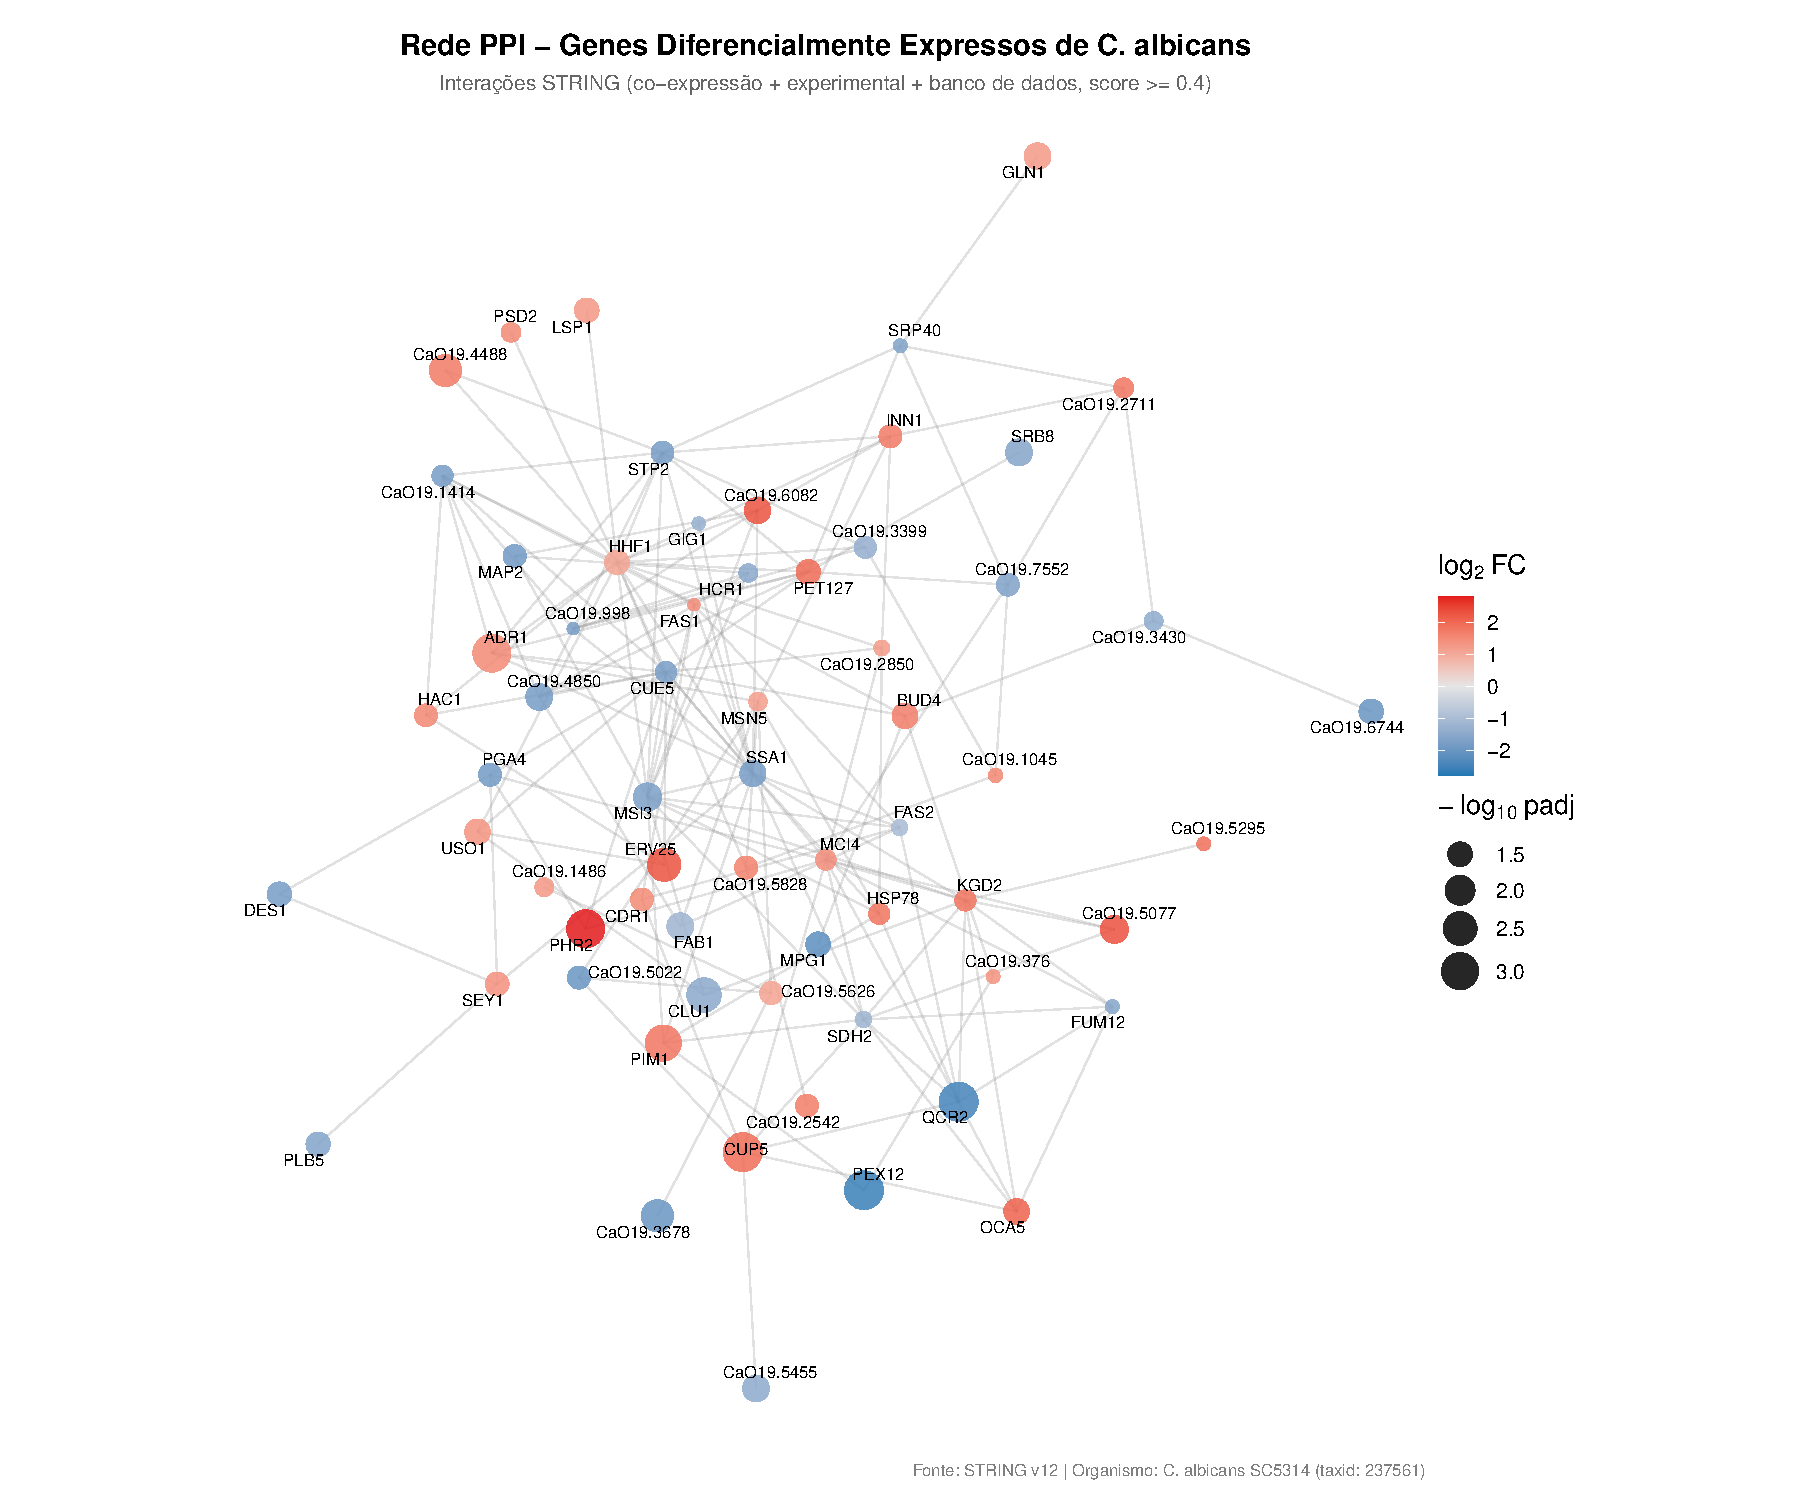
\includegraphics[keepaspectratio]{analysis/04_downstream_analyses_files/figure-pdf/unnamed-chunk-32-1.pdf}}

\subsection{Como interpretar a rede
PPI:}\label{como-interpretar-a-rede-ppi}

\begin{itemize}
\tightlist
\item
  \textbf{Cor dos nós}: segue uma escala contínua do \textbf{azul}
  (downregulado sob vancomicina) ao \textbf{vermelho} (upregulado),
  passando por cinza (log2FC próximo de zero). Isso permite identificar
  rapidamente se regiões da rede são dominadas por up ou downregulação.
\item
  \textbf{Tamanho dos nós}: proporcional a \(-\log_{10}(\text{padj})\)
  quanto maior o ponto, mais significativa é a mudança de expressão
  daquele gene.
\item
  \textbf{Arestas}: representam associações funcionais documentadas no
  STRING (co-expressão, evidência experimental ou bancos de dados
  curados). Arestas mais densas indicam sub-redes de proteínas que atuam
  de forma coordenada.
\item
  \textbf{Rótulos}: aparecem apenas para os 10\% dos genes mais
  significativos, destacando os candidatos de maior interesse biológico.
\item
  \textbf{Clusters visuais}: grupos de nós densamente conectados sugerem
  módulos funcionais --- conjuntos de proteínas que trabalham juntas em
  um processo biológico. Identifique se esses módulos correspondem às
  vias enriquecidas que encontramos anteriormente.
\end{itemize}

\begin{center}\rule{0.5\linewidth}{0.5pt}\end{center}

\textbf{Concluímos a análise completa de RNA-seq da \emph{Candida
albicans} em resposta à vancomicina. Desde a descontaminação das
leituras do hospedeiro com o nf-core/detaxizer, passando pela
quantificação com o nf-core/rnaseq, a análise de expressão diferencial
com DESeq2, o enriquecimento funcional com KEGG e GO, até a construção e
visualização de redes de interação proteína-proteína com o STRING ---
percorremos um pipeline completo e reprodutível para transcriptômica de
patógenos, enfrentando os desafios específicos de um organismo
não-modelo.}




\end{document}
